%!TEX root = ../main.tex
\section{Introduction}
\label{sec:intro}
%!TEX root = ../main.tex
\claudeinline{The introduction body is still empty --- the paper currently opens with \S1.1 (literature) with no
framing paragraph. Suggested content, one paragraph each: (1) the phenomenon (conditioning collapse at a compressed
clamped--free corner, first seen numerically, claimed here to be a corner-localised creasing bifurcation); (2) the
dichotomy result (tension benign / compression structural), with the two-scale tensile statement of
Theorem~\ref{thm:A}; (3) the reduction chain (blow-up to the $(\nu,\hat K)$ wedge, imperfect bifurcation, what is
proved vs.\ hypothesised --- the ledger of Table~\ref{tab:status} is the honest map); (4) relation to
Knowles--Sternberg, Ball, Biot/Hong, Kondratiev--Maz'ya \emph{with actual citations} --- \S1.1--1.2 currently cite by
name-and-decade in prose only, and \texttt{literature.bib} keys exist for several of these; (5) outline. Also: the
running example is 2D plane strain, and several results (screening Lemma~\ref{lem:screen}, existence
Lemma~\ref{lem:fundexist}) are genuinely two-dimensional (affine cofactor); the introduction should state up front
where $d=2$ is essential and where $d\ge3$ survives via the edge reduction of Proposition~\ref{prop:blowup}(iii).}


\subsection{Existing literature}
The literature on singularities in finite and nonlinear hyperelasticity is organised around three major phenomena.

\begin{itemize}
    \item \textbf{Crack tips in tension} (Knowles and Sternberg, 1970s). The classical work on nonlinear singularities
          treats a $360^\circ$ corner (a crack) pulled in pure tension. In a neo-Hookean material the asymptotic
          displacement field departs markedly from linear fracture mechanics; the analysis is, however, confined to
          traction-free boundaries and pure tensile opening.
    \item \textbf{Cavitation} (Ball, 1982). Under severe hydrostatic tension the hyperelastic equations admit singular
          weak solutions in which a hole opens spontaneously in the interior of a solid domain --- a point singularity
          with $\bm{F}\to\infty$.
    \item \textbf{Surface creasing} (Biot, 1963; Hong et al., 2009). A compressed flat half-space of neo-Hookean
          material becomes unstable at a critical stretch ($\lambda\approx0.54$); this instability is now understood as
          a \emph{crease}, a point singularity nucleating on an initially flat surface.
\end{itemize}

\subsection{The gap}
The existing nonlinear-singularity literature largely avoids the configuration of interest here: \emph{a geometric
corner (e.g.\ $90^\circ$) carrying mixed boundary conditions (Dirichlet meeting Neumann) under compression}. Each
strand addresses only part of it:

\begin{itemize}
    \item Linear theory (Kondratiev) handles the mixed-BC corner but ignores the large-deformation kinematics.
    \item Nonlinear theory (Knowles--Sternberg) handles large deformations but avoids the Dirichlet--Neumann condition
          and avoids compression.
    \item Instability theory handles compression but typically on flat domains or symmetric geometries, ignoring a
          pre-existing geometric corner singularity.
\end{itemize}

\noindent The open question this paper addresses is how an already-present stress concentration at a geometric
Dirichlet--Neumann corner couples with a nonlinear structural instability (buckling/creasing), and how the resulting
tangent operators can be bounded.

\section{Problem formulation}
\label{sec:formulation}

\subsection{Finite-strain elastostatics as energy minimisation}

We consider a hyperelastic body occupying a reference $d$-dimensional domain $\Omega \subset \mathbb{R}^d$ with
boundary $\partial\Omega = \overline{\Gamma_D} \cup \overline{\Gamma_N}$, $\Gamma_D \cap \Gamma_N = \emptyset$. The
deformation of the body is described by the displacement field $\bm{u} : \Omega \to \mathbb{R}^d$, the deformation map
$\bm{y}(\bm{x}) = \bm{x} + \bm{u}(\bm{x})$, and the associated deformation gradient
\begin{equation}
    \bm{F} = \Grad \bm{y} = \bm{I} + \Grad \bm{u}, \qquad J = \det \bm{F} > 0,
\end{equation}
where $\Grad$ denotes the gradient with respect to the reference configuration. The mechanical response is encoded
in a strain energy density $\Psi(\bm{F})$, and the equilibrium configuration is the minimiser of the total potential
energy
\begin{equation}
    \label{eq:totalenergy}
    \mathcal{E}(\bm{u}) = \int_\Omega \Psi(\bm{F})\,dV - \int_\Omega \bm{f}_0 \cdot \bm{u} \,dV - \int_{\Gamma_N} \bm{t}_0 \cdot \bm{u} \,dS,
\end{equation}
over the space of admissible displacements $U = \{ \bm{u} \in H^1(\Omega;\mathbb{R}^d) : \bm{u} = \bm{g} \text{ on } \Gamma_D \}$,
where $\bm{f}_0$ is a body force, $\bm{t}_0$ a prescribed traction on the Neumann boundary, and $\bm{g}$ the prescribed
boundary displacement. We seek $\bm{u} \in U$ such that $\mathcal{E}(\bm{u}) \le \mathcal{E}(\bm{v})$ for all admissible
$\bm{v}$.

\subsection{Stationarity, stress, and tangent modulus}

A minimiser satisfies the stationarity condition $D_{\delta \bm{u}}\mathcal{E}(\bm{u}) = 0$ for all admissible
variations $\delta \bm{u}$ (vanishing on $\Gamma_D$), which is the weak form of equilibrium
\begin{equation}
    \label{eq:weakform}
    \int_\Omega \bm{P}(\bm{F}) : \Grad \delta \bm{u} \,dV
    = \int_\Omega \bm{f}_0 \cdot \delta \bm{u} \,dV + \int_{\Gamma_N} \bm{t}_0 \cdot \delta \bm{u} \,dS,
\end{equation}
where the first Piola--Kirchhoff stress is the first derivative of the energy with respect to the deformation
gradient,
\begin{equation}
    \bm{P}(\bm{F}) = \frac{\partial \Psi}{\partial \bm{F}}.
\end{equation}
The natural boundary condition associated with $\Gamma_N$ is $\bm{P} \bm{N} = \bm{t}_0$, with $\bm{N}$ the reference
outward unit normal. Because \eqref{eq:weakform} is nonlinear in $\bm{u}$, it is solved iteratively by Newton's method.
Linearising the residual about a current iterate $\bar{\bm{u}}$ in a direction $\Delta \bm{u}$ introduces the
fourth-order tangent (elasticity) modulus $\mathbb{L}$, with components $L_{iJkL}$,
\begin{equation}
    \label{eq:tangentdef}
    \mathbb{L} = \frac{\partial \bm{P}}{\partial \bm{F}} = \frac{\partial^2 \Psi}{\partial \bm{F} \otimes \partial \bm{F}},
    \qquad L_{iJkL} = \frac{\partial^2 \Psi}{\partial F_{iJ}\,\partial F_{kL}},
\end{equation}
which possesses the major symmetry $L_{iJkL} = L_{kLiJ}$, so that each Newton step requires solving the linear problem
\begin{equation}
    \label{eq:newtonstep}
    \int_\Omega \Grad \delta \bm{u} : \mathbb{L}(\bar{\bm{F}}) : \Grad \Delta \bm{u} \,dV = -\,R(\bar{\bm{u}}; \delta \bm{u}),
\end{equation}
with $R(\bar{\bm{u}}; \delta \bm{u})$ the residual of \eqref{eq:weakform} evaluated at $\bar{\bm{u}}$. The well-posedness
and conditioning of \eqref{eq:newtonstep}---and hence the convergence of the whole nonlinear solver---are governed by
the coercivity and boundedness of the bilinear form induced by $\mathbb{L}(\bar{\bm{F}})$. The central object of this
work is therefore the behaviour of $\mathbb{L}$ as a function of the local deformation state.

\subsection{The neo-Hookean material}

To fix ideas and to exhibit explicit constants we use, as a running example, the compressible neo-Hookean strain energy
density adopted in the cut-finite-element study \cite{cutfemAD} that motivates this analysis,
\begin{equation}
    \label{eq:neohooke}
    \Psi(\bm{F}) = \frac{\mu_e}{2}\left( \tr(\bm{F}^T \bm{F}) - d \right) + f(J),
\end{equation}
where $\mu_e > 0$ is the shear modulus and $f(J)$ is a strictly convex volumetric penalty with $f(1) = 0$,
$f'(1) = -\mu_e$, and $f(J) \to \infty$ as $J \to 0^+$. Two standard choices are
\begin{equation}
    \label{eq:fchoices}
    f_{\log}(J) = -\mu_e \log J + \lambda_e \log^2 J,
    \qquad
    f_{\mathrm{quad}}(J) = \tfrac{\kappa}{2}(J-1)^2,
\end{equation}
with $\lambda_e$ the Lam\'e constant and $\kappa$ a bulk modulus; \eqref{eq:neohooke} with $f_{\log}$ reproduces the
model of \cite{cutfemAD}. The corresponding stress and tangent are
\begin{align}
    \bm{P}(\bm{F}) & = \mu_e \bm{F} + f'(J)\,J\,\bm{F}^{-T}, \\
    \label{eq:Lnh}
    L_{iJkL}       & = \mu_e\,\delta_{ik}\delta_{JL}
    + \left( f''(J)J^2 + f'(J)J \right) F^{-T}_{iJ} F^{-T}_{kL}
    - f'(J)J\, F^{-T}_{iL} F^{-T}_{kJ}.
\end{align}
The first term $\mu_e\,\delta_{ik}\delta_{JL}$ is constant; the entire nonlinear part is controlled by $J$ and the
\emph{inverse} deformation gradient $\bm{F}^{-1}$, yielding the structural bound
\begin{equation}
    \label{eq:Lbound}
    \| \mathbb{L}(\bm{F}) \| \le \mu_e + \Theta(J)\,\| \bm{F}^{-1} \|^2,
\end{equation}
where $\|\bm{F}^{-1}\| = \lambda_{\min}^{-1}$ is set by the smallest principal stretch and $\Theta$ is a scalar growth
function fixed by $f$ (computed explicitly in \S\ref{sub:growth}). Consequently $\mathbb{L}$ can become unbounded
through volumetric collapse, $\lambda_{\min} \to 0$ (equivalently $\bm{F}^{-1} \to \infty$); whether a purely tensile
blow-up of $\bm{F}$ (with $\bm{F}^{-1}$ bounded) leaves $\mathbb{L}$ finite depends on the growth of $\Theta(J)$, which
turns out to discriminate sharply between the two penalties in \eqref{eq:fchoices}. This dichotomy is the analytical
backbone of the present paper.

\subsection{The mixed-corner singularity}

The configuration of interest is a right-angle junction where the two boundary-condition types meet: a Dirichlet
face ($\Gamma_D$, prescribed displacement) abutting a traction-free Neumann face ($\Gamma_N$). In $\mathbb{R}^d$ this
junction is a codimension-two \emph{edge} $\Sigma$ (a point for $d=2$, a curve or surface for $d\ge3$); its transverse
geometry, in the two-plane normal to $\Sigma$, is the right-angle corner we analyse, and we use polar coordinates
$(r,\theta)$ in that transverse plane. Such junctions arise generically wherever a clamped face meets a traction-free
face --- for instance along the base edges of a compressed body, the concrete setting taken up in
Section~\ref{sec:concrete}. Classical Kondratiev/edge theory for the linearised problem predicts a transverse
singularity
\begin{equation}
    \bm{u}(r,\theta) \sim K\, r^{\alpha}\,\bm{\Phi}(\theta), \qquad \alpha \in (0,1),
\end{equation}
with $r$ the distance to the edge $\Sigma$, $K$ a generalised stress-intensity factor and
$\alpha$ the (geometry- and Poisson-ratio-dependent) singularity exponent. The deformation gradient then scales as
$\bm{F} = \bm{I} + \mathcal{O}(K r^{\alpha-1})$, so $\|\bm{F}\| \to \infty$ as $r \to 0$.

The question this raises---and which the remainder of the paper addresses---is how this kinematic singularity
propagates into the nonlinear tangent operator \eqref{eq:tangentdef}. In view of \eqref{eq:Lbound}, the answer hinges
on which principal stretch diverges: a tensile corner keeps $\bm{F}^{-1}$ bounded and (for a suitable penalty) leaves
$\mathbb{L}$ well behaved, whereas a compressive corner drives $\lambda_{\min} \to 0$ and blows up the \emph{norm} of
$\mathbb{L}$ (severe ill-conditioning). The tangent nonetheless remains strongly elliptic --- the compressive
instability is \emph{structural} (a corner analogue of creasing), not a change of type of the PDE. The following
sections analyse the two scenarios in turn (Section~\ref{sec:asymptotics}) and then show how a small imperfection
regularises the compressive case through a structural bifurcation (Section~\ref{sec:iba}).

\section{Asymptotic behaviour of the tangent operator at a mixed corner}
\label{sec:asymptotics}

\subsection{Geometry and linearised kinematics}

Let the reference domain $\Omega \subset \mathbb{R}^d$ ($d\ge2$) carry a right-angle Dirichlet--Neumann edge
$\Sigma$ of codimension two. Near a point of $\Sigma$ split $\mathbb{R}^d = T\Sigma \oplus \Pi$ into the edge tangent
space and the normal two-plane $\Pi$, and use polar coordinates $(r,\theta)$ in $\Pi$ with $r\in[0,R]$,
$\theta\in[0,\pi/2]$, where $r=\operatorname{dist}(\cdot,\Sigma)$. Write $B_\rho$ for the tubular neighbourhood
$\{\bm{x}\in\Omega : \operatorname{dist}(\bm{x},\Sigma)<\rho\}$ of the edge. The leading singularity is governed by the
transverse problem in $\Pi$, modulated smoothly along $\Sigma$; for $d=2$ the edge degenerates to a point and
$B_\rho$ to the corner disc.
\begin{itemize}
    \item \textbf{Dirichlet boundary ($\Gamma_D$):} $\theta = 0$, deformation prescribed, $\bm{y}(r,0) = \bm{g}(r)$.
    \item \textbf{Neumann boundary ($\Gamma_N$):} $\theta = \pi/2$, traction-free, $\bm{P}\bm{N} = \bm{0}$.
\end{itemize}

Classical Kondratiev theory for the \emph{linearised} problem gives the leading-order singular displacement
\begin{equation}
    \label{eq:kondratiev}
    \bm{u}(r,\theta) \sim K\, r^{\alpha}\,\bm{\Phi}(\theta),
\end{equation}
with $K$ the generalised stress-intensity factor (set by the far field), $\bm{\Phi}$ a smooth angular profile, and
$\alpha\in(0,1)$ the geometry- and Poisson-dependent exponent. Consequently
\begin{equation}
    \label{eq:Fblowup}
    \bm{F} = \bm{I} + \mathcal{O}\!\left(K\,r^{\alpha-1}\right), \qquad \|\bm{F}\|\to\infty \text{ as } r\to 0 .
\end{equation}
Whether this kinematic blow-up contaminates the tangent operator $\mathbb{L}=\partial^2\Psi/\partial\bm{F}\,\partial\bm{F}$
depends not on $\|\bm{F}\|$ but on which principal stretches diverge, which is the content of the rest of this section.

\subsection{Standing assumptions on the stored energy}

The mechanism we describe is not specific to the neo-Hookean model; that model only serves to fix ideas and to exhibit
explicit constants. We therefore phrase the analysis for a general frame-indifferent energy and isolate the structural
properties that the argument actually uses. Throughout, $\|\cdot\|$ denotes the operator (spectral) norm on tensors,
$0<\lambda_{\min}(\bm{F})\le\dots\le\lambda_{\max}(\bm{F})$ are the singular values of $\bm{F}$ (the $d$ principal
stretches), and we recall $\|\bm{F}^{-1}\| = \lambda_{\min}(\bm{F})^{-1}$.

\begin{assumption}[Regularity and frame indifference]
    \label{ass:reg}
    The stored energy $\Psi:\mathrm{GL}^+(d)\to\mathbb{R}$ is objective, $\Psi\in C^2(\mathrm{GL}^+(d))$, and
    $\Psi(\bm{F})\to+\infty$ as $\det \bm{F}\to 0^+$.
\end{assumption}

\begin{assumption}[Inverse-channel growth of the tangent]
    \label{ass:growth}
    There exist a continuous, nondecreasing function $\Theta:(0,\infty)\to(0,\infty)$ and a constant $c_0\ge 0$ such
    that the tangent modulus $\mathbb{L}(\bm{F})=D^2\Psi(\bm{F})$ satisfies, for all $\bm{F}\in\mathrm{GL}^+(d)$,
    \begin{equation}
        \label{eq:Hessbound}
        \| \mathbb{L}(\bm{F}) \| \;\le\; c_0 \;+\; \Theta\!\big(\det \bm{F}\big)\,\|\bm{F}^{-1}\|^{2}.
    \end{equation}
\end{assumption}

\begin{assumption}[Uniform strong ellipticity on bounded-distortion sets]
    \label{ass:ellip}
    For every $0<c\le 1$ and $M\ge 1$ there is $\gamma(c,M)>0$ such that whenever $\lambda_{\min}(\bm{F})\ge c$ and
    $\det \bm{F}\le M$,
    \begin{equation}
        \label{eq:LH}
        L_{iJkL}(\bm{F})\, m_i N_J\, m_k N_L \;\ge\; \gamma(c,M)\,|\bm{m}|^2\,|\bm{N}|^2
        \qquad \forall\, \bm{m},\bm{N}\in\mathbb{R}^2 .
    \end{equation}
\end{assumption}

The decisive feature of Assumption~\ref{ass:growth} is that the inverse-stretch factor
$\|\bm{F}^{-1}\|^2=\lambda_{\min}^{-2}$ is the \emph{only} algebraic channel through which the Hessian can blow up; the
dependence on $\|\bm{F}\|$ (equivalently on $\lambda_{\max}$) enters solely through the scalar $\Theta(\det \bm{F})$.
Whether a tensile corner ($\lambda_{\max}\to\infty$, $\det \bm{F}\to\infty$, $\lambda_{\min}$ bounded below) is benign
therefore reduces to the \emph{growth rate} of $\Theta$, which we quantify in \S\ref{sub:growth}. Materials with
genuine tensile stiffening of the deviatoric part (Gent, Arruda--Boyce), whose tangent diverges through
$\lambda_{\max}$ directly rather than through $\Theta(\det\bm F)$, violate \eqref{eq:Hessbound} and are excluded.

\begin{lemma}[Assumptions for the neo-Hookean model]
    \label{lem:nh}
    Let $\Psi$ be the neo-Hookean energy \eqref{eq:neohooke} with $\mu_e>0$ and $f\in C^2(0,\infty)$. Then
    Assumption~\ref{ass:growth} holds with $c_0=\mu_e$ and
    \begin{equation}
        \label{eq:Thetagen}
        \Theta(J) = \big|\,f''(J)J^2 + f'(J)J\,\big| + \big|\,f'(J)J\,\big|,
    \end{equation}
    and Assumption~\ref{ass:ellip} holds on the convexity set $\{f''(J)\ge0\}$ --- in particular on all of compression
    $J\le1$ and moderate tension for $f_{\log}$, and globally for $f_{\mathrm{quad}}$ ($f''=\kappa>0$); it can fail under
    extreme dilation $J>J_*$ for $f_{\log}$ (Remark~\ref{rem:SEcaveat}). Assumption~\ref{ass:reg}
    additionally requires the barrier property $f(J)\to\infty$ as $J\to0^+$: this holds for $f_{\log}$ but \emph{fails}
    for $f_{\mathrm{quad}}$, since $f_{\mathrm{quad}}(J)\to\tfrac{\kappa}{2}<\infty$ (see Remark~\ref{rem:quad} and
    Scenario~B).
\end{lemma}

\begin{proof}
    Objectivity and $C^2$ regularity on $\mathrm{GL}^+(d)$ are immediate; the barrier hypothesis $f(J)\to\infty$ as
    $J\to0^+$, when assumed, gives the blow-up required by Assumption~\ref{ass:reg}. In \eqref{eq:Lnh} the first term is
    the scaled identity, of norm $\mu_e$. Each
    of the remaining two terms is a rank-one, respectively transposition, contraction of $\bm{F}^{-T}\otimes\bm{F}^{-T}$;
    since $\|\bm{F}^{-T}\|=\|\bm{F}^{-1}\|$, each is bounded in operator norm by its scalar prefactor times
    $\|\bm{F}^{-1}\|^2$. The triangle inequality gives \eqref{eq:Hessbound} with $c_0=\mu_e$ and $\Theta$ as in
    \eqref{eq:Thetagen}. For Assumption~\ref{ass:ellip}, contracting \eqref{eq:Lnh} with $\bm{m}\otimes\bm{N}$ and
    writing $\xi:=\bm{m}\cdot\bm{F}^{-T}\bm{N}=\bm{N}\cdot\bm{F}^{-1}\bm{m}$, the two volumetric terms combine
    ($(f''J^2+f'J)\xi^2-f'J\,\xi^2$) to the single clean form
    \begin{equation}
        \label{eq:LHnh}
        L_{iJkL}m_iN_Jm_kN_L = \mu_e\,|\bm{m}|^2|\bm{N}|^2 + f''(J)\,J^2\,\xi^2 .
    \end{equation}
    Wherever $f''(J)\ge0$ the second term is nonnegative and \eqref{eq:LH} holds with $\gamma=\mu_e$, uniformly in
    $\bm{F}$ (no distortion bound needed); this covers $f_{\mathrm{quad}}$ ($f''=\kappa>0$) everywhere and $f_{\log}$ on
    $\{f''_{\log}\ge0\}$. \qed
\end{proof}

\begin{remark}[Strength and a tension caveat]
    \label{rem:SEcaveat}
    Identity \eqref{eq:LHnh} is sharper than \eqref{eq:LH}: the neo-Hookean tangent is strongly elliptic with constant
    \emph{exactly} $\mu_e$ wherever $f''(J)\ge0$, and the volumetric term only adds to it. The Hessian of the quadratic
    (Hookean) part is constant, which is why the \emph{deviatoric} response never blows up; only the \emph{volumetric}
    response, through $\Theta$, can. One caveat for $f_{\log}$: since
    $f''_{\log}(J)=(\mu_e+2\lambda_e-2\lambda_e\log J)/J^2$, convexity is lost once
    $J>J_*:=\exp\!\big(1+\mu_e/(2\lambda_e)\big)$, and then \eqref{eq:LHnh} can turn negative for $\xi$ near its maximal
    value $|\bm{m}||\bm{N}|/\lambda_{\min}$. Hence Assumption~\ref{ass:ellip} holds throughout \emph{compression}
    ($J\le1$) and moderate tension, but $f_{\log}$ can lose strong ellipticity under \emph{extreme dilation}
    ($J>J_*$)---a tension-side phenomenon distinct from the compressive analysis, and one more reason the bounded-$J$
    qualifier matters in \S\ref{sub:scenarioA}. The globally convex $f_{\mathrm{quad}}$ is free of this.
\end{remark}

\subsection{The non-compressive hypothesis}

The qualitative split between the two scenarios is captured by a single quantity: the smallest principal stretch near
the corner. We call the corner singularity \emph{non-compressive} when $\lambda_{\min}$ stays bounded away from zero,
even though $\lambda_{\max}$ (hence $\|\bm{F}\|$ and $\det\bm{F}$) may diverge.

\begin{assumption}[Non-compressive singularity, (NC)]
    \label{ass:nc}
    There exist $\rho\in(0,R]$ and $c\in(0,1]$ such that the equilibrium deformation satisfies
    \begin{equation}
        \label{eq:NC}
        \lambda_{\min}(\bm{F}(\bm{x})) \ge c, \quad\text{equivalently}\quad \|\bm{F}^{-1}(\bm{x})\|\le c^{-1},
        \qquad \text{for a.e. } \bm{x}\in B_\rho .
    \end{equation}
\end{assumption}

We stress what \eqref{eq:NC} does \emph{not} say. It does not require incompressibility, and crucially it does
\emph{not} bound $\det\bm{F}$: in a tensile corner $\lambda_{\max}\sim r^{\alpha-1}\to\infty$, so
$J=\det\bm{F}=\prod_i\lambda_i\sim r^{\alpha-1}\to\infty$ as well (one diverging stretch, the remaining $d-1$ bounded).
The only quantity (NC) controls is
$\|\bm{F}^{-1}\|\le c^{-1}$. Physically, (NC) states that the material is pulled around the corner (tension/shear)
rather than crushed into it. Because $\det\bm{F}$ is \emph{not} bounded under (NC), the factor $\Theta(\det\bm{F})$ in
\eqref{eq:Hessbound} need not stay bounded; the next subsection makes its growth explicit, and this is precisely where
the two volumetric penalties \eqref{eq:fchoices} part ways. Scenario~B (\S\ref{sub:scenarioB}) treats the
complementary, compressive case in which \eqref{eq:NC} fails.

\subsection{Explicit volumetric growth functions}
\label{sub:growth}

The bound \eqref{eq:Hessbound} exposes \emph{two independent channels} through which the tangent can diverge, and they
are kinematically decoupled:
\begin{equation}
    \label{eq:twochannels}
    \|\mathbb{L}(\bm{F})\| \le \mu_e
    + \underbrace{\Theta(\det\bm{F})}_{\substack{\text{dilation channel}\\ J\to\infty}}\;\cdot\;
    \underbrace{\|\bm{F}^{-1}\|^{2}}_{\substack{\text{inverse channel}\\ \lambda_{\min}\to 0}} .
\end{equation}
The \emph{inverse channel} is the one usually blamed for trouble: it requires $\lambda_{\min}\to0$, i.e. compression to
zero volume, and is the subject of Scenario~B. The \emph{dilation channel}, $\Theta(\det\bm{F})\to\infty$ as
$J\to\infty$, is activated by \emph{expansion} and is precisely what a tensile corner switches on, since
$\lambda_{\max}\sim r^{\alpha-1}\to\infty$ forces $J\to\infty$ even with $\lambda_{\min}$ bounded below by (NC). Whether
this matters is therefore not a property of the corner or of the sign of the loading, but of the \emph{growth rate of
    $\Theta$}---a property of the volumetric penalty $f$ alone. We now evaluate it for the two penalties
\eqref{eq:fchoices}; the contrast shows that ``tension is benign'' is a model-dependent statement.

\paragraph{Logarithmic penalty.}
For $f_{\log}(J)=-\mu_e\log J+\lambda_e\log^2 J$,
\begin{equation}
    f'(J)J = -\mu_e + 2\lambda_e\log J,
    \qquad
    f''(J)J^2 = \mu_e + 2\lambda_e - 2\lambda_e\log J,
\end{equation}
so that the combination collapses to a constant,
\begin{equation}
    \label{eq:logcombo}
    f''(J)J^2 + f'(J)J = 2\lambda_e,
\end{equation}
and therefore
\begin{equation}
    \label{eq:Thetalog}
    \Theta_{\log}(J) = 2\lambda_e + \big|\,2\lambda_e\log J - \mu_e\,\big| = \mathcal{O}\!\big(\log J\big)
    \quad\text{as } J\to\infty .
\end{equation}
The volumetric stiffening grows only \emph{logarithmically} in $J$.

\paragraph{Quadratic penalty.}
For $f_{\mathrm{quad}}(J)=\tfrac{\kappa}{2}(J-1)^2$,
\begin{equation}
    f'(J)J = \kappa J(J-1),
    \qquad
    f''(J)J^2 = \kappa J^2,
    \qquad
    f''(J)J^2 + f'(J)J = \kappa J(2J-1),
\end{equation}
so
\begin{equation}
    \label{eq:Thetaquad}
    \Theta_{\mathrm{quad}}(J) = \kappa J\,|2J-1| + \kappa J\,|J-1| = \mathcal{O}\!\big(\kappa J^2\big)
    \quad\text{as } J\to\infty .
\end{equation}
The volumetric stiffening grows \emph{quadratically} in $J$.

\paragraph{Consequence at the corner.}
We combine \eqref{eq:Hessbound} with (NC) ($\|\bm{F}^{-1}\|^2\le c^{-2}$) and the tensile kinematics. In the
non-compressive regime exactly one stretch diverges: $\lambda_{\max}\sim|K|\,r^{\alpha-1}$ while the remaining $d-1$
stretches stay bounded (in particular $\lambda_{\min}$ bounded below), so $J=\det\bm{F}=\prod_i\lambda_i\sim
r^{\alpha-1}$. (If instead $\Grad\bm{u}$ had two diverging eigenvalues, the corresponding subdeterminant would give
$J\sim r^{2(\alpha-1)}$; we work in the one-large-stretch regime characteristic of a Dirichlet--Neumann opening, where
$J\sim r^{\alpha-1}$.) The tangent norm near the corner then obeys
\begin{equation}
    \label{eq:Lcornergrowth}
    \|\mathbb{L}(\bm{x})\| \le \mu_e + c^{-2}\,\Theta\!\big(\det\bm{F}(\bm{x})\big) \sim
    \begin{cases}
        \mu_e + \mathcal{O}\!\big(\log\tfrac1r\big), & f=f_{\log},          \\[4pt]
        \mathcal{O}\!\big(r^{-2(1-\alpha)}\big),     & f=f_{\mathrm{quad}}.
    \end{cases}
\end{equation}
Thus the logarithmic penalty keeps the tangent bounded up to a logarithm, whereas the quadratic penalty produces a
genuine \emph{algebraic} blow-up of the tangent \emph{even in pure tension}. This is the dilation channel of
\eqref{eq:twochannels} acting alone, with the inverse channel inert ($\|\bm{F}^{-1}\|$ bounded); it is algebraically
singular of a severity comparable to---though mechanistically distinct from---the compressive blow-up of Scenario~B,
which instead runs through $\|\bm{F}^{-1}\|^2$. The often-repeated statement that ``tension is harmless for
neo-Hookean'' is therefore an artefact of the logarithmic volumetric model and is false for the quadratic one.

\paragraph{Physical reading: the large-dilation response.}
The dichotomy is, at bottom, a statement about how the bulk energy behaves under unbounded \emph{expansion}, the
loading a tensile corner imposes:
\begin{center}
    \begin{tabular}{lll}
        \toprule
        volumetric model           & energy as $J\to\infty$   & tangent $\Theta(J)$   \\
        \midrule
        $\lambda_e\log^2 J$        & $\sim \log^2 J$ \ (soft) & $\mathcal{O}(\log J)$ \\
        $\tfrac{\kappa}{2}(J-1)^2$ & $\sim J^2$ \ (stiff)     & $\mathcal{O}(J^2)$    \\
        \bottomrule
    \end{tabular}
\end{center}
A penalty that is polynomial in $J$ makes the material resist further dilation ever more stiffly, and the linearised
modulus faithfully reports that stiffness as a blow-up; the logarithmic penalty is gentle about expansion and does not.
Both penalties are designed to diverge correctly as $J\to0$ (resisting collapse, the inverse channel); their
large-$J$ behaviour, which the dilation channel probes, was never physically constrained, and that latitude is exactly
where they part. The exact cancellation \eqref{eq:logcombo} is the analytic signature of this softness. We make the
benign case precise in Theorem~\ref{thm:A} and flag the algebraic case in Remark~\ref{rem:quad}.

\subsection{Scenario A: the tensile (non-compressive) singularity}
\label{sub:scenarioA}

We work under the mild-growth condition isolated above.

\begin{assumption}[Mild volumetric growth]
    \label{ass:mild}
    The growth function satisfies $\Theta(J) = \mathcal{O}\!\big((\log J)^{p}\big)$ as $J\to\infty$ for some $p\ge 0$.
\end{assumption}

\noindent By \eqref{eq:Thetalog}, $f_{\log}$ satisfies Assumption~\ref{ass:mild} with $p=1$; by \eqref{eq:Thetaquad},
$f_{\mathrm{quad}}$ does not.

\begin{lemma}[Subordinate tangent]
    \label{lem:Abound}
    Under Assumptions~\ref{ass:reg}, \ref{ass:growth}, \ref{ass:mild} and (NC), for every $\varepsilon>0$ there is
    $C_\varepsilon$ with
    \begin{equation}
        \label{eq:subord}
        \|\mathbb{L}(\bm{x})\| \le C_\varepsilon\, r^{-\varepsilon} \qquad \text{for a.e. } \bm{x}\in B_\rho .
    \end{equation}
    In particular $\mathbb{L}\in L^q(B_\rho)$ for every $q<\infty$, and $\|\mathbb{L}\|$ is dominated by any negative
    power of $r$.
\end{lemma}

\begin{proof}
    By \eqref{eq:Hessbound} and (NC), $\|\mathbb{L}\|\le \mu_e + c^{-2}\Theta(\det\bm{F})$. Assumption~\ref{ass:mild}
    and $\det\bm{F}=\mathcal{O}(r^{\alpha-1})$ give $\Theta(\det\bm{F})=\mathcal{O}\big((\log\tfrac1r)^p\big)$, and
    $(\log\tfrac1r)^p\le C_\varepsilon r^{-\varepsilon}$ on $(0,\rho]$ for every $\varepsilon>0$. \qed
\end{proof}

\begin{lemma}[Strong ellipticity outside the dilation core]
    \label{lem:Aellip}
    Let $f=f_{\log}$ and let $J_*=\exp\!\big(1+\mu_e/(2\lambda_e)\big)$ be the dilation threshold of
    Remark~\ref{rem:SEcaveat}, beyond which $f''_{\log}<0$. Under Assumptions~\ref{ass:reg}, \ref{ass:ellip} and (NC),
    with the tensile kinematics $J\sim|K|\,r^{\alpha-1}$ of \S\ref{sub:growth}, define the \emph{dilation core radius}
    \begin{equation}
        \label{eq:rstar}
        r_*:=\big(J_*/|K|\big)^{1/(\alpha-1)}=\big(|K|/J_*\big)^{1/(1-\alpha)} ,
    \end{equation}
    so that $J(\bm{x})\le J_*$ for $r\ge r_*$. Then on the annular region $A_*:=\{\bm{x}\in B_\rho: r_*<r<\rho\}$ the
    tangent satisfies the Legendre--Hadamard condition with the \emph{constant} ellipticity modulus $\mu_e$,
    \begin{equation}
        \label{eq:LHcorner}
        L_{iJkL}(\bm{x})\,m_iN_Jm_kN_L \ \ge\ \mu_e\,|\bm{m}|^2|\bm{N}|^2
        \qquad \text{for a.e. } \bm{x}\in A_*,\ \ \forall\,\bm{m},\bm{N}\in\mathbb{R}^2.
    \end{equation}
    On the complementary core $\{r\le r_*\}$, where $J>J_*$, the constant-modulus bound \eqref{eq:LHcorner} no longer
    holds, and strong ellipticity of $f_{\log}$ \emph{can} fail (Remark~\ref{rem:SEcaveat}): wherever the sharper
    condition $|f''(J)|J^2\,\|\bm{F}^{-1}\|^2>\mu_e$ is met, the directional modulus
    $\mu_e+f''(J)J^2\,\xi^2/(|\bm m|^2|\bm N|^2)$ turns negative for $\xi$ near its maximum. We do not claim the loss is
    pointwise throughout the core --- only that the core is where it can occur, since $f''(J)J^2<0$ there is necessary
    for it.
\end{lemma}

\begin{proof}
    By the exact rank-one identity \eqref{eq:LHnh},
    \begin{equation*}
        L_{iJkL}m_iN_Jm_kN_L = \mu_e\,|\bm{m}|^2|\bm{N}|^2 + f''(J)\,J^2\,\xi^2,
        \qquad \xi:=\bm{m}\cdot\bm{F}^{-T}\bm{N},
    \end{equation*}
    in which the volumetric prefactor is the single scalar $f''(J)J^2=\mu_e+2\lambda_e-2\lambda_e\log J$
    (cf.~\eqref{eq:logcombo}). This is nonnegative precisely when $\log J\le 1+\mu_e/(2\lambda_e)$, i.e. $J\le J_*$.
    Since $J\sim|K|r^{\alpha-1}$ is decreasing in $r$ (recall $\alpha<1$), the threshold $J=J_*$ is crossed at the single
    radius \eqref{eq:rstar}, and $J\le J_*$ throughout $A_*$. There the second term only adds to $\mu_e$, giving
    \eqref{eq:LHcorner}. For $r<r_*$ we have $J>J_*$, hence $f''(J)J^2<0$; taking $\bm{m},\bm{N}$ aligned so that
    $\xi^2$ attains its maximum $|\bm{m}|^2|\bm{N}|^2\,\|\bm{F}^{-1}\|^2$ (admissible since $\|\bm{F}^{-1}\|\le c^{-1}$ is
    only an upper bound, with equality possible) drives the form below zero once
    $|f''(J)J^2|\,\|\bm{F}^{-1}\|^2>\mu_e$. \qed
\end{proof}

\noindent The picture is therefore sharper, and more honest, than ``tension is harmless'': for the logarithmic penalty
the tensile corner is strongly elliptic on the annulus $A_*$ outside a \emph{dilation core} $\{r\le r_*\}$, inside which
$f_{\log}$ itself --- not the corner --- \emph{may} cease to be strongly elliptic because the material is dilated past
$J_*$ (where the sharper condition $|f''(J)|J^2\|\bm F^{-1}\|^2>\mu_e$ binds). The
core radius $r_*$ in \eqref{eq:rstar} shrinks as the threshold $J_*=\exp(1+\mu_e/(2\lambda_e))$ grows, i.e. as the
penalty is made stiffer against extreme dilation (large $\lambda_e/\mu_e$); a model with $f''\ge0$ globally would have
$r_*=0$ and no core. This is the tensile mirror of the model-dependence already seen for $\Theta$ in
\S\ref{sub:growth}, and it confines the genuinely delicate behaviour to a controlled inner region.

For the weighted well-posedness we recall two standard inequalities in the Kondratiev space
$V^{1,2}_\beta(B_\rho)$---the closure of smooth functions vanishing on $\Gamma_D\cap\partial B_\rho$ under
$\|\bm{v}\|_{V^{1,2}_\beta}^2 = \int_{B_\rho} \big(r^{2\beta}|\Grad\bm{v}|^2 + r^{2\beta-2}|\bm{v}|^2\big)\,dV$.

\begin{lemma}[Weighted Hardy and Korn inequalities {\cite{KMR2001,NazarovPlamenevsky1994}}]
    \label{lem:korn}
    Let $\beta\in\mathbb{R}$ avoid the (discrete) set of exceptional exponents of the corner. There are constants
    $C_H, C_K$ depending only on $\beta$ and the opening angle such that, for all $\bm{v}\in V^{1,2}_\beta(B_\rho)$
    vanishing on $\Gamma_D\cap\partial B_\rho$,
    \begin{align}
        \label{eq:hardy}
        \int_{B_\rho} r^{2\beta-2}|\bm{v}|^2\,dV    & \le C_H \int_{B_\rho} r^{2\beta}|\Grad\bm{v}|^2\,dV,                \\
        \label{eq:korn}
        \int_{B_\rho} r^{2\beta}|\Grad\bm{v}|^2\,dV & \le C_K \int_{B_\rho} r^{2\beta}\,|\bm{\varepsilon}(\bm{v})|^2\,dV,
        \qquad \bm{\varepsilon}(\bm{v}) = \tfrac12\big(\Grad\bm{v}+\Grad\bm{v}^T\big).
    \end{align}
\end{lemma}

Let $\beta_\star$ be the weight exponent for which the \emph{linear} elasticity corner problem at this
Dirichlet--Neumann junction is Fredholm (equivalently $\beta_\star$ avoids the singular exponents $\alpha$). The
existence of such a weight, and the resulting Fredholm property in the weighted space $V^{1,2}_{\beta_\star}$, is the
standard Kondratiev--Maz'ya--Nazarov--Plamenevsky theory for elliptic systems with conical/edge singularities
\cite{KMR2001,NazarovPlamenevsky1994}: the operator is Fredholm precisely when $\beta_\star$ avoids the discrete
spectrum of the corner operator pencil (the singular exponents), and the resolvent is then compact, so the spectrum is
discrete and the critical mode $\bm{\phi}$ of Assumption~\ref{ass:bif} is genuinely attained. We may
write the Newton-step bilinear form as
\begin{equation}
    \label{eq:formA}
    a(\Delta\bm{u},\delta\bm{u}) := \int_{B_\rho} \Grad\delta\bm{u} : \mathbb{L}(\bar{\bm{F}}) : \Grad\Delta\bm{u}\,dV .
\end{equation}

\begin{theorem}[Well-posedness of the linearised step, tensile corner]
    \label{thm:A}
    Under Assumptions~\ref{ass:reg}--\ref{ass:mild} and the non-compressive hypothesis (NC), the Newton-step form
    \eqref{eq:formA} is bounded and coercive modulo a compact perturbation: on any region $\Omega$ on which the tangent
    is strongly elliptic with the constant Legendre--Hadamard modulus $\mu_e$ (Lemma~\ref{lem:Aellip}), there exist
    constants $\Lambda<\infty$, $\gamma_1>0$ and a compact form $k(\cdot,\cdot)$ such that, for all
    $\bm{u},\bm{v}\in V^{1,2}_{\beta_\star}(\Omega)$,
    \begin{align}
        \label{eq:Abounded}
        |a(\bm{u},\bm{v})| & \le \Lambda\,\|\bm{u}\|_{V^{1,2}_{\beta_\star}}\,\|\bm{v}\|_{V^{1,2}_{\beta_\star}}, \\
        \label{eq:Agaarding}
        a(\bm{v},\bm{v})   & \ge \gamma_1\,\|\bm{v}\|_{V^{1,2}_{\beta_\star}}^2 - k(\bm{v},\bm{v}).
    \end{align}
    The consequences split according to whether the vertex lies in the elliptic region.

    \emph{(A) Globally convex-volumetric barrier ($f''\ge0$ together with the standing
    Assumptions~\ref{ass:reg}--\ref{ass:mild}, e.g.\ $f_{\log}$ with a finite-extensibility cap $J_{\max}\le J_*$ on the
    dilation).} Then the dilation core is empty, $r_*=0$, ellipticity holds on the \emph{full} corner
    neighbourhood $\Omega=B_\rho$ \emph{including the vertex}, and \eqref{eq:Abounded}--\eqref{eq:Agaarding} hold on
    $V^{1,2}_{\beta_\star}(B_\rho)$. Hence the linearised corner operator is Fredholm of index zero in
    $V^{1,2}_{\beta_\star}(B_\rho)$; for $\beta_\star$ avoiding the corner spectrum it is an isomorphism, its solutions
    admit the Kondratiev asymptotic expansion \eqref{eq:kondratiev} at the vertex, and the governing singular exponents
    coincide with those of the linearised elasticity problem. This is the genuine corner result.

    \emph{(B) Logarithmic barrier $f_{\log}$ ($r_*>0$).} The vertex sits inside the non-elliptic core $\{r\le r_*\}$
    (Lemma~\ref{lem:Aellip}), so the estimates hold only on the \emph{vertex-free} annulus $\Omega=A_*=\{r_*<r<\rho\}$.
    There the operator is a regular uniformly elliptic problem: \eqref{eq:Abounded}--\eqref{eq:Agaarding} give
    Fredholmness of index zero in $V^{1,2}_{\beta_\star}(A_*)$ and well-posedness on the annulus, but \emph{no}
    corner-pencil asymptotics are asserted across the inner boundary $r=r_*$, which is a smooth interface carrying no
    vertex, not a conical point. The vertex behaviour of $f_{\log}$ is the open inner problem of Remark~\ref{rem:core}.
    In the mild-loading limit $r_*\downarrow0$ (small $|K|$) the core shrinks below any fixed scale and the conclusion
    of (A) is recovered on every fixed sub-annulus down to mesh resolution.
\end{theorem}

\begin{proof}
    The bounds \eqref{eq:Abounded}--\eqref{eq:Agaarding} are established on the elliptic region $\Omega$ ($=B_\rho$ in
    case (A), $=A_*$ in case (B)); the case split affects only whether the vertex is interior to $\Omega$, hence whether
    the Kondratiev corner analysis applies.

    \emph{Boundedness.} By Cauchy--Schwarz and Lemma~\ref{lem:Abound}, on $\Omega$ the coefficient obeys the sharp bound
    $\|\mathbb{L}\|\le\mu_e+c^{-2}\Theta(J)=\mu_e+\mathcal{O}\!\big(\log\tfrac1r\big)$, a \emph{logarithm}, not a power.
    Hence for every $\delta>0$ there is $C_\delta$ with $\|\mathbb{L}\|\le C_\delta\,r^{-\delta}$, and
    \begin{align*}
        |a(\bm{u},\bm{v})|
         & \le \int_{\Omega} \|\mathbb{L}\|\,|\Grad\bm{u}|\,|\Grad\bm{v}|\,dV
        \le C_\delta \Big(\!\int_{\Omega} r^{2\beta_\star}|\Grad\bm{u}|^2\Big)^{1/2}
        \Big(\!\int_{\Omega} r^{-2\delta-2\beta_\star}|\Grad\bm{v}|^2\Big)^{1/2}.
    \end{align*}
    This exhibits $a$ as bounded from $V^{1,2}_{\beta_\star}\times V^{1,2}_{-\beta_\star-\delta}$ (the dual pairing
    $V^{1,2}_{\beta_\star}\times V^{1,2}_{-\beta_\star}$ with a $\delta$ of weighted slack). The logarithm is
    subordinate to \emph{every} algebraic weight, so the loss may be made smaller than the slack to the weight interval:
    let $(\beta_-,\beta_+)$ be the maximal open interval of weights for which the \emph{linear} corner pencil has no
    eigenvalue with $\Re$-part in $[\beta_\star-\delta,\beta_\star]$ (such a $\delta$-band exists because $\beta_\star$
    avoids the discrete corner spectrum, hence sits at a positive distance $\delta_0$ from it). Choose $\delta<\delta_0$,
    so $\beta_\star-\delta$ lies in the same admissible interval as $\beta_\star$. In case (B) the domain $\Omega=A_*$
    excludes the vertex, the two Kondratiev norms $V^{1,2}_{\beta_\star}$ and $V^{1,2}_{-\beta_\star-\delta}$ are then
    comparable (they differ only at the vertex, which $A_*$ omits), and \eqref{eq:Abounded} follows directly with
    $\Lambda=\Lambda(\delta)$. In case (A) the vertex is interior to $\Omega=B_\rho$ and the two norms are \emph{not}
    comparable there, so the same-space estimate is obtained by perturbation off the constant-coefficient symbol rather
    than by norm comparison. Write $\mathbb{L}=\mathbb{L}_{\mathrm{lin}}+\mathbb{R}$, with $\mathbb{L}_{\mathrm{lin}}$
    the frozen linear-elasticity tensor at the vertex (whose pencil is Fredholm in $V^{1,2}_{\beta_\star}(B_\rho)$ for
    $\beta_\star$ off the corner spectrum, by Kondratiev--Maz'ya theory \cite{KMR2001}) and
    $\mathbb{R}=\mathbb{L}-\mathbb{L}_{\mathrm{lin}}=\mathcal{O}(\log\tfrac1r)$ the nonlinear correction. The hypotheses
    of the relevant stability theorem are exactly: (a) $\mathbb{L}_{\mathrm{lin}}$ is strongly elliptic and its pencil
    has no eigenvalue on $\Re\lambda=\beta_\star$; and (b) $\mathbb{R}$ is \emph{subordinate} to the principal part,
    $\|\mathbb{R}\|=o(r^{-\delta})$ for every $\delta>0$ (Lemma~\ref{lem:Abound}), hence of relative bound $0$ with
    respect to the Hardy-weighted graph norm. Both are met here, so the standard subordinate-perturbation theorem of
    \cite{KMR2001} applies: the admissible weight interval is unmoved and the \emph{full} pair of estimates
    \eqref{eq:Abounded}--\eqref{eq:Agaarding} --- not boundedness alone --- transfers from $\mathbb{L}_{\mathrm{lin}}$
    to $\mathbb{L}$ on $V^{1,2}_{\beta_\star}(B_\rho)$. In both cases the logarithmic growth does not shift the
    admissible interval; no singular weight is ``absorbed'' into $\bm{v}$.

    \emph{G\aa rding inequality.} By Lemma~\ref{lem:Aellip} the symbol $\mathbb{L}(\bm{x})$ is strongly elliptic on
    $\Omega$ with the constant Legendre--Hadamard modulus $\mu_e$. Freezing the (measurable, uniformly elliptic)
    coefficients on a dyadic partition $\{r\sim 2^{-j}\}\cap \Omega$ and applying the constant-coefficient G\aa rding
    inequality on each annulus---valid because the principal symbol is positive definite on the Legendre--Hadamard
    cone---yields, after summation against the weight $r^{2\beta_\star}$,
    \[
        a(\bm{v},\bm{v}) \ge \mu_e\,c_K^{-1}\!\int_{\Omega} r^{2\beta_\star}|\Grad\bm{v}|^2\,dV
        - C\!\int_{\Omega} r^{2\beta_\star}|\bm{v}|^2\,dV,
    \]
    where the step from Legendre--Hadamard positivity to coercivity is the classical one for strongly elliptic systems:
    strong ellipticity with modulus $\mu_e$ (Lemma~\ref{lem:Aellip}) gives the constant-coefficient G\aa rding bound for
    the symmetrised gradient $\bm{\varepsilon}(\bm v)$ on each frozen annulus, and the weighted Korn inequality
    \eqref{eq:korn} then converts control of $\bm{\varepsilon}(\bm v)$ into control of the full gradient $\Grad\bm v$.
    The remainder term has a strictly higher power of $r$ than the Hardy weight $r^{2\beta_\star-2}$, hence by
    \eqref{eq:hardy} it is relatively compact with respect to $\|\cdot\|_{V^{1,2}_{\beta_\star}}$; this is the compact form
    $k$, and we obtain \eqref{eq:Agaarding} with $\gamma_1=\mu_e\, c_K^{-1}$.

    \emph{Fredholm property and exponents.} Estimates \eqref{eq:Abounded}--\eqref{eq:Agaarding} place the operator in the
    Kondratiev--Maz'ya framework \cite{KMR2001}: it is Fredholm of index zero in $V^{1,2}_{\beta_\star}(\Omega)$ whenever
    $\beta_\star$ avoids the spectrum of the corner operator pencil. In case (A), where $\Omega=B_\rho$ contains the
    vertex, this is a genuine corner statement: because the nonlinear correction to the principal symbol is subordinate
    (it is $o(r^{-\delta})$ for every $\delta$, by Lemma~\ref{lem:Abound}), the pencil coincides with that of linearised
    elasticity, and its eigenvalues are exactly the exponents $\alpha$ of \eqref{eq:kondratiev}, unchanged by the
    nonlinearity. In case (B), where $\Omega=A_*$ omits the vertex, the same estimates give Fredholmness and
    well-posedness on the annulus, but the inner boundary $r=r_*$ is a smooth interface, not a conical point, so the
    pencil eigenvalues describe no vertex asymptotics there; the corner expansion \eqref{eq:kondratiev} is recovered only
    in the limit $r_*\downarrow0$ on fixed sub-annuli, and the genuine vertex theory for $f_{\log}$ remains the open
    inner problem of Remark~\ref{rem:core}. \qed
\end{proof}

\begin{remark}[The dilation core]
    \label{rem:core}
    For $f_{\log}$ the conclusion of Theorem~\ref{thm:A} is genuinely confined to $A_*$: the vertex itself sits inside the
    core $\{r\le r_*\}$, where $J>J_*$ and $f_{\log}$ is not strongly elliptic. Three readings are consistent with the
    analysis. (i) \emph{Mild loading}: for stress-intensity $|K|$ small the core radius $r_*=(|K|/J_*)^{1/(1-\alpha)}$ is
    so small that the corner is elliptic on all of $B_\rho$ down to mesh scale, and the theorem governs the entire
    computationally resolved region. (ii) \emph{Sharper model statement}: the tensile corner ``passes like linear
    elasticity'' on $A_*$, and the only obstruction is the material law's own loss of ellipticity past $J_*$---a property
    of $f_{\log}$, not of the corner. (iii) \emph{Open inner problem}: a complete vertex theory for $f_{\log}$ requires a
    separate analysis inside the non-elliptic core, which we leave open; a globally convex-volumetric barrier
    ($f''\ge0$, $r_*=0$) removes the issue entirely and recovers the unrestricted statement. Physically, the loss of
    ellipticity past $J_*$ is an artefact of the unbounded dilation that $f_{\log}$ permits: real polymer networks reach
    \emph{finite extensibility}, and a volumetric law that caps the dilation, $J<J_{\max}$ (the bulk analogue of the
    Gent deviatoric model), with $J_{\max}\le J_*$ keeps $f''>0$ throughout the attainable range and so eliminates the
    core. The dilation core is thus a feature of the specific large-$J$ tail of $f_{\log}$, not a physical catastrophe.
\end{remark}

\begin{remark}[Stress is singular, operator is not]
    The first Piola--Kirchhoff stress still blows up, $\bm{P}\sim \mu_e\bm{F}\to\infty$ as $r\to0$, so the tensile corner
    is a genuine \emph{stress} singularity. Theorem~\ref{thm:A} asserts only that, on the annulus $A_*$, this singularity
    lives entirely in the \emph{right-hand side} (the residual) of the Newton step, not in its operator: under a mild
    volumetric penalty the nonlinear problem inherits the regularity theory of the linear one, standard graded meshes
    restore optimal convergence, and no structural instability occurs. This is the precise sense in which a
    non-compressive corner ``passes like linear elasticity'' away from the dilation core.
\end{remark}

\begin{remark}[The quadratic penalty does \emph{not} pass like linear elasticity]
    \label{rem:quad}
    For $f_{\mathrm{quad}}$, Assumption~\ref{ass:mild} fails: by \eqref{eq:Thetaquad} and \eqref{eq:Lcornergrowth} the
    tangent grows algebraically, $\|\mathbb{L}\|=\mathcal{O}(r^{-2(1-\alpha)})$, \emph{even in pure tension}. The
    coefficients of \eqref{eq:formA} are then genuinely singular, of severity comparable to the compressive Scenario~B,
    the boundedness step above fails for $\beta_\star$, and the admissible weight interval---hence the effective corner
    exponents seen by the nonlinear operator---shifts relative to linear elasticity. A sharp analysis of this case (the
    correct weight, and whether coercivity survives) is governed by the volumetric blow-up rather than by the
    deviatoric singularity and is left open here.

    We emphasise that this serves as a \emph{cautionary comparator} rather than a model we advocate: as written,
    $f_{\mathrm{quad}}'(1)=0\ne-\mu_e$, so $\tfrac{\kappa}{2}(J-1)^2$ does not combine with the deviatoric term
    $\tfrac{\mu_e}{2}(\tr(\bm{F}^T\bm{F})-d)$ to leave the reference configuration stress-free, and in practice it is used
    together with an isochoric (deviatoric/volumetric) split of $\bm{F}$. The point is that a standard-looking polynomial
    penalty already forfeits the benign tensile behaviour enjoyed by the logarithmic model \eqref{eq:fchoices} actually
    used in \cite{cutfemAD}.
    %TODO: decide whether to develop the quadratic-penalty weighted analysis or cite it as motivation for preferring the
    %      logarithmic volumetric model in computations.
\end{remark}

\begin{remark}[Self-consistency of (NC)]
    Hypothesis (NC) is compatible with the singular kinematics \eqref{eq:Fblowup}: an angular profile $\bm{\Phi}$
    corresponding to opening/shear produces $\Grad\bm{u}$ whose dominant eigenvalue is positive (radial extension), so
    $\lambda_{\max}\to\infty$ while $\lambda_{\min}=\det\bm{F}/\lambda_{\max}$ need not approach zero. The complementary
    profile, in which the dominant eigenvalue of $\Grad\bm{u}$ is negative, drives $\lambda_{\min}\to0$ and violates
    (NC); that is exactly Scenario~B below.
\end{remark}

\subsection{Scenario B: the compressive singularity (the pathological case)}
\label{sub:scenarioB}

Now assume the far-field loading pushes the material \emph{into} the corner ($K < 0$, radial compression).

\paragraph{Kinematic consequence.}
The naive linear prediction gives $\Grad\bm{u}$ a negative dominant eigenvalue scaling as $-|K| r^{\alpha-1}$. Because
$\bm{F} = \bm{I} + \Grad\bm{u}$, as $r \to 0$ (or as the pseudo-time load factor $t$ increases) there is a critical
threshold where the local contraction annihilates the material volume:
\begin{equation}
    \det \bm{F} \to 0 \implies J \to 0, \qquad \lambda_{\min} \to 0 .
\end{equation}

\paragraph{Operator blow-up (and its model dependence).}
Here it is the \emph{inverse channel} of \eqref{eq:twochannels} that fires: $\|\bm{F}^{-1}\| = \lambda_{\min}^{-1} \to
    \infty$. The dilation channel $\Theta(J)$ is now probed at $J\to0^+$ rather than $J\to\infty$, and---exactly as in
tension, but with the roles reversed---its behaviour discriminates between the two penalties. Writing
$J=\prod_i\lambda_i\sim\lambda_{\min}$ near the corner (one collapsing stretch, the remaining $d-1$ bounded, cf.
\S\ref{sub:growth}),
\begin{equation}
    \label{eq:Thetacompress}
    \Theta_{\log}(J) \sim 2\lambda_e\,\big|\log J\big| \to \infty,
    \qquad
    \Theta_{\mathrm{quad}}(J) \sim 2\kappa J \to 0
    \qquad (J\to 0^+),
\end{equation}
so that the tangent norm $\|\mathbb{L}\|\le \mu_e + \Theta(J)\|\bm{F}^{-1}\|^2$ behaves as
\begin{equation}
    \label{eq:Lcompress}
    \| \mathbb{L}(\bm{x}) \| \sim
    \begin{cases}
        \mathcal{O}\!\big(\lambda_{\min}^{-2}\,\log\tfrac1{\lambda_{\min}}\big), & f=f_{\log},          \\[4pt]
        \mathcal{O}\!\big(\lambda_{\min}^{-1}\big),                              & f=f_{\mathrm{quad}}.
    \end{cases}
\end{equation}
Thus the logarithmic penalty---benign under tension---produces here the \emph{stronger} blow-up, $\lambda_{\min}^{-2}$
\emph{amplified} by a logarithm, whereas the quadratic penalty gives the milder rate $\lambda_{\min}^{-1}$. This
reversal is not a redemption of the quadratic model: $f_{\mathrm{quad}}(J)\to\tfrac{\kappa}{2}<\infty$ as $J\to0^+$, so
it provides \emph{no energy barrier against volume collapse} and violates Assumption~\ref{ass:reg}; the milder tangent
growth merely reflects this missing barrier (the material is free to interpenetrate at finite energy), which is a worse
pathology, not a better one. The logarithmic penalty's stronger blow-up is, conversely, the analytic price of a genuine
barrier $f_{\log}(J)\to+\infty$---and it is precisely that barrier which forces, and gives physical meaning to, the
bifurcation rescue of Section~\ref{sec:iba}.

\paragraph{Ellipticity is \emph{not} lost --- the instability is structural.} It is tempting to attribute the breakdown to a loss of strong ellipticity (an
indefinite acoustic tensor). For this neo-Hookean model that is \emph{false}, and it is worth stating the fact
precisely, as it shapes the rest of the analysis.

\begin{lemma}[Compressive strong ellipticity of the neo-Hookean tangent]
    \label{lem:SEcompress}
    For the energy \eqref{eq:neohooke}, the rank-one form of the tangent is exactly \eqref{eq:LHnh},
    $L_{iJkL}m_iN_Jm_kN_L=\mu_e|\bm{m}|^2|\bm{N}|^2+f''(J)J^2(\bm{m}\cdot\bm{F}^{-T}\bm{N})^2$. Wherever $f''(J)\ge0$ ---
    in particular throughout compression, $J\le1$, for both penalties \eqref{eq:fchoices} --- the tangent is strongly
    elliptic with constant $\ge\mu_e>0$, uniformly in $\bm{F}$, and the acoustic tensor $Q_{ik}(\bm{N})=L_{iJkL}N_JN_L$
    is positive definite and never degenerates under compression.
\end{lemma}

\begin{proof}
    The identity is \eqref{eq:LHnh} (Lemma~\ref{lem:nh}). As $J\to0^+$, $f''(J)J^2\to+\infty$ for $f_{\log}$
    (cf.~\eqref{eq:fppblow}) and $f''(J)J^2=\kappa J^2\ge0$ for $f_{\mathrm{quad}}$; in both cases the second term only
    \emph{adds} to the constant $\mu_e$. \qed
\end{proof}

Thus the compressive corner is \emph{not} a material instability: the volumetric stiffening that blows up
$\|\mathbb{L}\|$ is exactly the term $f''(J)J^2$ in \eqref{eq:LHnh}, and it is positive --- it strengthens ellipticity
while destroying conditioning. What fails is the \emph{boundedness} of the operator, not its positivity.

\paragraph{Conclusion for Scenario B.}
The assumption that the deformation smoothly follows the fundamental path into the corner therefore produces, not a
loss of ellipticity, but two distinct effects: (i) a blow-up of the tangent \emph{norm}, $\|\mathbb{L}\|\to\infty$
(eq.~\eqref{eq:Lcompress}), which renders the Newton step catastrophically ill-conditioned even though it remains
elliptic; and (ii) for a barrier penalty $f_{\log}$, an unphysical infinite accumulation of energy ($f(J)\to\infty$ as
$J\to0$), signalling that the smooth fundamental path is not the physical solution. The genuine mechanism that
intervenes is a \emph{structural} bifurcation of the compressed state --- the corner analogue of \emph{creasing}, an
instability of a material that remains everywhere strongly elliptic (Lemma~\ref{lem:SEcompress}), driven by the
geometry and boundary conditions rather than by a change of type of the PDE. To capture it we introduce in
Section~\ref{sec:iba} an imperfect perturbation that regularises the bifurcation and bounds the singularity; we work
from here on with the barrier model $f_{\log}$, for which collapse is genuinely resisted.

\section{Imperfect bifurcation analysis and asymptotic bounds}
\label{sec:iba}

The previous section showed that the perfect compressive path drives $\lambda_{\min}\to0$ and blows up the tangent norm
while the material remains strongly elliptic (Lemma~\ref{lem:SEcompress}), so the breakdown is a structural instability
rather than a loss of type. The premise of this section is that this scenario is an idealisation: a real system always
carries small disturbances---geometric imperfections, load eccentricities, material inhomogeneity---and these select a
nearby \emph{regular} solution branch on which the collapse never quite happens. We model the disturbance by a single
scalar amplitude $\epsilon$, carry out an imperfect-bifurcation analysis, and quantify how the tangent blows up as
$\epsilon\to0$. The punchline is that the blow-up is confined to a vanishingly small neighbourhood of the corner and
proceeds at a controlled algebraic rate, so that for every $\epsilon>0$ the problem is regular.

\subsection{The regularised problem and the fundamental path}

We localise to the corner neighbourhood $B_\rho$ of \S\ref{sec:asymptotics}, regard the loading as transmitted through
data on the outer arc $\partial B_\rho\setminus(\Gamma_D\cup\Gamma_N)$, and introduce a pseudo-time load parameter
$t\in[0,1]$ that monotonically scales the compressive part of that data. Following the answer to the question posed in
Scenario~B, we add a small, fixed volumetric body force $\epsilon\,\bm{p}(\bm{x})$ with $\|\bm{p}\|_{L^2(B_\rho)}=1$
and $\epsilon\ll1$ as the imperfection (we write the field as $\bm{p}$ to avoid collision with the penalty $f(J)$). The
regularised equilibrium is $G(\bm{u},t,\epsilon)=0$,
\begin{equation}
    \label{eq:Gdef}
    \langle G(\bm{u},t,\epsilon),\bm{v}\rangle = \int_{B_\rho} \bm{P}(\bm{F}) : \Grad\bm{v}\,dV
    - \epsilon \int_{B_\rho} \bm{p}\cdot\bm{v}\,dV - \ell_t(\bm{v}) = 0 \qquad \forall\,\bm{v}\in V,
\end{equation}
with $\bm{P}=\partial\Psi/\partial\bm{F}$, $V$ the admissible test space, and $\ell_t$ the (linear) load functional at
pseudo-time $t$. Let $\bm{u}_0(t)$ denote the \emph{fundamental path}, i.e. the branch of \eqref{eq:Gdef} with
$\epsilon=0$ that continues the low-load compressive solution. We use the barrier penalty $f_{\log}$ throughout, so the
collapse $J\to0$ is genuinely resisted (Assumption~\ref{ass:reg}); along $\bm{u}_0(t)$ the corner stretch
$\lambda_c(t):=\lambda_{\min}(\bm{F}_0(t))$ decreases as $t\uparrow1$ but, on the bifurcating branch we construct, never
reaches zero.

\begin{remark}[The instability is structural, not material]
    \label{rem:framework}
    By Lemma~\ref{lem:SEcompress} the tangent stays strongly elliptic throughout compression, so the bifurcation here is
    a \emph{structural} one (a buckling of the boundary-value problem), not a material change of type. We work with the
    global form on the bounded domain $B_\rho$. The operator $\mathcal{L}(t)=\partial_{\bm{u}}G(\bm{u}_0(t),t,0)$ has
    discrete spectrum and attains $\mu_1(t)$ as a genuine eigenvalue \emph{provided} the fundamental stretch stays
    bounded away from collapse up to the crossing, $\inf_{B_\rho}\lambda_{\min}(\bm{F}_0(t))\ge c>0$ for $t\le t_c$: then
    $\mathcal{L}(t)$ has \emph{bounded} strongly-elliptic coefficients on the bounded domain, hence (G\aa rding, Korn and
    the Rellich embedding) compact resolvent --- we make this precise as Lemma~\ref{lem:attain} in the concrete setting.
    The reservation is essential: what makes the problem delicate is not a loss of ellipticity but the \emph{norm}
    blow-up $\|\mathbb{L}\|\to\infty$ (eq.~\eqref{eq:Lcompress}), and it is exactly this blow-up, through the
    scale-invariant (creasing) corner, that would push the bottom of the spectrum into the \emph{essential} spectrum and
    destroy attainment. Crucially, that blow-up occurs only on the unphysical continuation past $t_c$, where
    $\lambda_{\min}\to0$; at the crossing itself the spectrum is discrete \emph{so long as buckling precedes collapse}.
    The coercivity constant thus stays positive while the boundedness constant diverges, and the crossing eigenvalue
    $\mu_1(t)$ and the conditioning are controlled by different mechanisms. Assumption~\ref{ass:bif} records the spectral
    facts (attainment and simplicity) we use; \S\ref{sub:core} shows that, for the concrete model, both follow once
    buckling is known to precede collapse.
\end{remark}

\subsection{What is provable, and what must be assumed}

It is worth separating the genuinely provable facts about the critical point from the irreducible hypotheses. Let
$Q_t(\bm{v}):=\int_{B_\rho}\Grad\bm{v}:\mathbb{L}(\bm{F}_0(t)):\Grad\bm{v}\,dV$ be the second-variation form on the
fundamental path and $\mu_1(t):=\inf_{\|\bm{v}\|_V=1}Q_t(\bm{v})$.

\paragraph{The critical load exists (conditionally provable).}
A clarification is essential here. By Lemma~\ref{lem:SEcompress} the neo-Hookean material remains strongly elliptic
throughout compression, so $\mu_1(t)$ \emph{cannot} be driven negative by a rank-one (material) instability: any
crossing must be a \emph{structural} loss of positivity of the global form $Q_t$, i.e. a buckling of the boundary-value
problem in which the destabilising test field is not rank-one. This is the creasing mechanism.
\begin{lemma}[Existence of the critical load]
    \label{lem:tc}
    Assume (i) coercivity at zero load, $\mu_1(0)>0$, and (ii) a structural instability of the compressed state: there
    exist $t_*\in(0,1)$ and $\bm{v}_*\in V$ with $Q_{t_*}(\bm{v}_*)<0$. Then $\mu_1$ is continuous on $[0,t_*]$ and there
    is a first $t_c\in(0,t_*]$ with $\mu_1(t_c)=0$ and $\mu_1(t)>0$ for $t<t_c$.
\end{lemma}
\begin{proof}
    At $t=0$, $\bm{F}_0=\bm{I}$ and $\mathbb{L}=\mu_e\mathbb{I}+(\text{volumetric at }J{=}1)$ is positive definite, so
    with Korn's inequality $\mu_1(0)>0$. Hypothesis (ii) gives $\mu_1(t_*)\le Q_{t_*}(\bm{v}_*)/\|\bm{v}_*\|_V^2<0$. As
    $t\mapsto\mathbb{L}(\bm{F}_0(t))$ is continuous, so is $\mu_1$, and the intermediate value theorem gives the first
    zero $t_c$. \qed
\end{proof}
\noindent Hypothesis (i) is provable for neo-Hookean (positive-definiteness at $\bm{F}=\bm{I}$ plus Korn). Hypothesis
(ii) --- the existence of a structurally destabilising field --- is the genuine content and is \emph{not} elementary: it
is the corner counterpart of the Biot/creasing instability \cite{Biot1963,Hong2009} and we do not establish it here.

\paragraph{The critical mode (assumed).}
\begin{assumption}[Critical mode]
    \label{ass:bif}
    At $t_c$ the infimum $\mu_1(t_c)=0$ is attained at a mode $\bm{\phi}\in V$, $\|\bm{\phi}\|_V=1$, spanning a
    one-dimensional, isolated kernel of $\mathcal{L}_c$ (the rest of the spectrum bounded away from $0$), with
    $\bm{\phi}$ supported in the edge neighbourhood $B_\rho$.
\end{assumption}
\noindent This bundles two spectral facts: \emph{attainment} (the minimising sequence does not escape into the
corner as essential spectrum) and \emph{simplicity}. Simplicity is generic and, for the model bodies, can be argued
from the lateral \emph{face-preserving} reflection $R$ of \S\ref{sub:symmetry} (\emph{not} the corner bisector
$\theta\mapsto\tfrac\pi2-\theta$, which swaps $\Gamma_D$ and $\Gamma_N$ and is no symmetry of the mixed problem);
attainment is the borderline-elliptic difficulty flagged in
Remark~\ref{rem:framework}. Neither is irreducible: in the concrete setting attainment is \emph{proved}
(Lemma~\ref{lem:attain}) and simplicity is reduced to genericity \emph{within} the symmetry sector carrying the
critical mode (\S\ref{sub:symmetry}), the only residue being the cleaner geometric condition that buckling
precede pointwise collapse.

\paragraph{The crossing is transversal (provable under monotone loading).}
\begin{lemma}[Transversality]
    \label{lem:transversal}
    Suppose the loading is monotonically destabilising at $t_c$,
    \begin{equation}
        \label{eq:monotone}
        \langle\bm{\phi},\dot{\mathbb{L}}(t_c)\bm{\phi}\rangle
        := \int_{B_\rho}\Grad\bm{\phi}:\partial_t\mathbb{L}(\bm{F}_0(t_c)):\Grad\bm{\phi}\,dV < 0 . \tag{M}
    \end{equation}
    Then, under Assumption~\ref{ass:bif}, $\mu_1$ is differentiable at $t_c$ with
    $a:=-\mu_1'(t_c)=-\langle\bm{\phi},\dot{\mathbb{L}}(t_c)\bm{\phi}\rangle>0$.
\end{lemma}
\begin{proof}
    For a simple eigenvalue, first-order perturbation theory gives $\mu_1'(t_c)=\langle\bm{\phi},\dot{\mathbb{L}}(t_c)\bm{\phi}\rangle$;
    hypothesis \eqref{eq:monotone} fixes the sign. \qed
\end{proof}
\noindent Condition \eqref{eq:monotone} is the precise meaning of ``more compression $\Rightarrow$ less stiffness in
the buckling direction'' and holds for any monotone compressive load path; it is an input on the \emph{loading}, not on
the solution.

\paragraph{The imperfection is active (provable, generic).}
\begin{lemma}[Generic activation]
    \label{lem:eta}
    For every $\bm{p}$ outside the closed codimension-one subspace $\bm{\phi}^\perp$, the projection
    $\eta:=\int_{B_\rho}\bm{p}\cdot\bm{\phi}\,dV\neq0$. Hence $\eta\neq0$ for generic imperfection.
\end{lemma}

\begin{remark}[Universality of the imperfection]
    \label{rem:imperfuniv}
    The volumetric body force $\epsilon\,\bm{p}$ is chosen only for concreteness; the analysis depends on the
    imperfection \emph{solely} through the scalar $\eta=\langle\bm{p},\bm{\phi}\rangle$, so any perturbation with a
    nonzero $\bm{\phi}$-projection produces the identical reduced equation \eqref{eq:bifeq}. Indeed, write a generic
    imperfect equilibrium as $G(\bm{u},t,0)=\epsilon\,\bm{h}$ with $\bm{h}\in V'$ the (linearised) imperfection
    functional. A boundary-traction defect on $\Gamma_N$ contributes $\bm{h}(\bm{v})=\int_{\Gamma_N}\bm{t}_1\cdot\bm{v}\,dS$;
    a geometric imperfection --- rounding the corner with radius $\sim\epsilon$, or a small shape variation
    $\bm{x}\mapsto\bm{x}+\epsilon\,\bm{\theta}(\bm{x})$ --- enters, after pulling back to the reference domain, as a
    fixed load functional $\bm{h}(\bm{v})=\int_{B_\rho}\mathbb{S}[\bm{\theta}]:\Grad\bm{v}\,dV$ linear in the shape field
    $\bm{\theta}$. In every case the kernel projection $\langle G,\bm{\phi}\rangle=0$ yields the same normal form with
    $\eta$ replaced by $\langle\bm{h},\bm{\phi}\rangle$, nonzero for $\bm{h}$ outside the closed codimension-one subspace
    $\bm{\phi}^\perp$ (Lemma~\ref{lem:eta}). The Koiter $\tfrac23$ law \eqref{eq:koiter} and all subsequent bounds are
    therefore universal across generic imperfections, not an artefact of the body-force model.
\end{remark}

\paragraph{The nonlinearity is explicit; only the sign of its orthogonal-mode feedback is open.}
For the neo-Hookean model the reduced coefficients are not opaque. By Lemma~\ref{lem:volcoeff} the deviatoric energy is
quadratic and drops out, so every coefficient of order $\ge3$ is purely volumetric; moreover the quadratic coefficient
$c_2:=\tfrac12\langle\bm{\phi},\partial^2_{\bm{u}}G[\bm{\phi},\bm{\phi}]\rangle$ vanishes \emph{identically} for a mode
antisymmetric under the lateral, face-preserving reflection $R$ of \S\ref{sub:symmetry} --- not the corner bisector
$\theta\mapsto\tfrac\pi2-\theta$, which swaps $\Gamma_D$ and $\Gamma_N$ and is no symmetry at all. What these
structural facts do \emph{not} settle is the \emph{sign} of the cubic and quintic coefficients; indeed, by
Lemma~\ref{lem:volcoeff}(ii), the explicit single-mode (frozen) parts point \emph{against} subcriticality,
$b_{\mathrm{dir}}>0$ and $d_{\mathrm{dir}}<0$ in compression. The subcritical pattern therefore hinges on the
geometry-dependent orthogonal-mode feedback overturning these signs; we record it as a residual hypothesis to be
verified numerically (Remark~\ref{rem:bsign}) rather than asserted from the creasing analogy
\cite{Biot1963,Hong2009}.
\begin{assumption}[Subcritical sign pattern (residual, geometry-dependent)]
    \label{ass:subcrit}
    With $c_2=0$ by Lemma~\ref{lem:volcoeff}(i), the full reduced cubic and quintic coefficients
    \begin{equation}
        b:=\tfrac16\langle\bm{\phi},\partial^3_{\bm{u}}G[\bm{\phi},\bm{\phi},\bm{\phi}]\rangle,
        \qquad
        d:=\tfrac1{120}\langle\bm{\phi},\partial^5_{\bm{u}}G[\bm{\phi},\dots,\bm{\phi}]\rangle,
    \end{equation}
    each the frozen part of Lemma~\ref{lem:volcoeff} corrected by the orthogonal-mode feedback, satisfy $b<0<d$
    (subcritical with quintic saturation). This is a condition on the corner geometry, not on the material model.
\end{assumption}
\begin{remark}[Status of the subcritical signs: geometry-decided, checked numerically]
    \label{rem:bsign}
    Assumption~\ref{ass:subcrit} is the one genuinely residual hypothesis of the construction, and
    Lemma~\ref{lem:volcoeff} localises exactly where its content lies. The deviatoric response and the quadratic
    coefficient are settled ($c_2=0$, no feedback correction); the cubic and quintic decompose as
    $b=b_{\mathrm{dir}}+b_\psi$ and $d=d_{\mathrm{dir}}+d_\psi$, with the single-mode parts explicit and, in
    compression, of definite but \emph{adverse} sign ($b_{\mathrm{dir}}=2\!\int_{B_\rho} f''(J_0)d_\phi^2\,dV>0$,
    $d_{\mathrm{dir}}=\!\int_{B_\rho} f'''(J_0)d_\phi^3\,dV<0$). The corrections $b_\psi,d_\psi$ are the
    Lyapunov--Schmidt feedback through the orthogonal complement $V^\perp$: quadratic forms in the second-order field
    $\bm\psi$ that depend on the opening angle, the Dirichlet--Neumann arrangement and the mode $\bm\phi$ --- on the
    geometry, not on $f$. Subcriticality thus requires $b_\psi$ to overturn the explicit positive $b_{\mathrm{dir}}$
    (and likewise for $d$). The reason this does not reduce to a single universal corner number is a homogeneity count
    (Proposition~\ref{prop:bcount}, \S\ref{sub:bcount}): the clamped--free edge exponent satisfies $\alpha>\tfrac12$, so
    the cubic integral is convergent at the tip but \emph{not} dominated by it, leaving an $\mathcal{O}(1)$ dependence on
    the normalised stress-intensity $\hat K$; the sign of $b$ is therefore a function $b(\nu,\hat K)$ on the model wedge
    rather than an inheritance from flat creasing. The \emph{direction} of the cubic feedback can in fact be signed
    analytically: $b_\psi\le0$ always, by the variational structure of the first crossing
    (Lemma~\ref{lem:fbsign} below), so the genuinely open content is the magnitude comparison
    $|b_\psi|>b_{\mathrm{dir}}$; the quintic feedback $d_\psi$ we do not sign. The magnitude is evaluated
    numerically from the eigenmode and reduced operator of the two-dimensional model wedge of Proposition~\ref{prop:blowup}
    as a function of $(\nu,\hat K)$, which is the proper arbiter of a geometry-dependent sign. Were the verdict $b>0$ instead, the bifurcation would be supercritical and \emph{more}
    benign --- the physical branch smooth through $t_c$ with no snap at onset --- and the regularisation conclusions of
    \S\ref{sub:core} and Proposition~\ref{prop:narrow} would hold a fortiori; the complementary transcritical case
    $c_2\neq0$ is covered in Remark~\ref{rem:transcritical}.
\end{remark}

\subsection{Lyapunov--Schmidt reduction}

\begin{proposition}[Normal form]
    \label{prop:LS}
    Under Assumption~\ref{ass:bif}, Lemma~\ref{lem:transversal} and Assumption~\ref{ass:subcrit}, there is a
    neighbourhood of $(\bm{u}_0(t_c),t_c,0)$ in which the solutions of \eqref{eq:Gdef} are exactly
    \begin{equation}
        \bm{u}(t,\epsilon) = \bm{u}_0(t) + w\,\bm{\phi} + \bm{\psi}(w,t,\epsilon),
        \qquad \bm{\psi}\in V^\perp:=\{\bm{\phi}\}^{\perp},
    \end{equation}
    where $\bm{\psi}$ is smooth with $\bm{\psi}=\mathcal{O}(w^2+\epsilon)$, and the amplitude $w$ solves the scalar
    imperfect bifurcation equation, retained to quintic order because the cubic is destabilising ($b<0$),
    \begin{equation}
        \label{eq:bifeq}
        a\,(t_c-t)\,w + b\,w^3 + d\,w^5 = \epsilon\,\eta + \mathcal{O}\!\big(\epsilon^2 + \epsilon w + |t_c-t|\,w^2 + w^6\big),
    \end{equation}
    with $a>0$ (Lemma~\ref{lem:transversal}), $b<0<d$ (Assumption~\ref{ass:subcrit}) and $\eta$ as in
    Lemma~\ref{lem:eta}.
\end{proposition}

\begin{proof}
    Let $P$ be the $V$-orthogonal projection onto $\operatorname{span}\{\bm{\phi}\}$ and $Q=I-P$. Write
    $\bm{u}=\bm{u}_0(t)+w\bm{\phi}+\bm{\psi}$ with $\bm{\psi}\in V^\perp$. The range equation $Q\,G=0$ has invertible
    linearisation $Q\,\mathcal{L}_c\,Q$ on $V^\perp$ by Assumption~\ref{ass:bif}, so the implicit function theorem
    yields a unique smooth $\bm{\psi}=\bm{\psi}(w,t,\epsilon)$ with $\bm{\psi}(0,t_c,0)=0$ and
    $\bm{\psi}=\mathcal{O}(w^2+\epsilon+|t_c-t|)$. Substituting into the kernel equation $\langle G,\bm{\phi}\rangle=0$
    and Taylor-expanding $G$ about $(\bm{u}_0(t_c),t_c,0)$ gives \eqref{eq:bifeq}: the linear term $a(t_c-t)w$ from
    Lemma~\ref{lem:transversal}, the cubic $bw^3$ and quintic $dw^5$ from Assumption~\ref{ass:subcrit} (the quadratic
    vanishing by symmetry), and the inhomogeneity $\epsilon\eta$ from $-\epsilon\langle\bm{p},\bm{\phi}\rangle$. Because
    $b<0$, the cubic alone does not saturate the amplitude, which is why the quintic $dw^5$ ($d>0$) is retained. \qed
\end{proof}

\subsection{The sign of the orthogonal-mode feedback is not free}
\label{sub:fbsign}

Assumption~\ref{ass:subcrit} bundles two logically distinct statements about the cubic: that the Lyapunov--Schmidt
feedback $b_\psi$ \emph{opposes} the frozen part ($b_\psi\le0$, against $b_{\mathrm{dir}}>0$ of
Lemma~\ref{lem:volcoeff}(ii)), and that it does so with sufficient \emph{magnitude}, $|b_\psi|>b_{\mathrm{dir}}$. The
first is not a hypothesis at all: at the first crossing it is a theorem, forced by the variational structure alone. We
record it here, both because it halves the open content of Assumption~\ref{ass:subcrit} and because it converts the
numerical verification of \S\ref{sec:numerical} from a sign determination into a magnitude comparison, with a
certification principle (Corollary~\ref{cor:cert}) that requires no inversion of the reduced operator.

Because the load terms in \eqref{eq:Gdef} are linear in $\bm{u}$, $G$ is a gradient,
$G(\bm{u},t,\epsilon)=D\mathcal{E}_t(\bm{u})-\epsilon\,\bm{p}$ with $\mathcal{E}_t$ the total energy at load $t$; write
$E_k:=D^k\mathcal{E}_{t_c}\big(\bm{u}_0(t_c)\big)$ for the symmetric $k$-th variation at the critical point, so that
$\mathcal{L}_c=E_2$, $\partial^2_{\bm{u}}G=E_3$ and $\partial^3_{\bm{u}}G=E_4$ there.

\begin{lemma}[The feedback is never adverse]
    \label{lem:fbsign}
    Let $t_c$ be the first crossing of Lemma~\ref{lem:tc} and let Assumption~\ref{ass:bif} hold, with $\delta>0$ the
    spectral gap of $\mathcal{L}_c$ above its one-dimensional kernel $\operatorname{span}\{\bm{\phi}\}$. Define
    $R\in(V^\perp)'$ by
    \begin{equation}
        \label{eq:Rdef}
        \langle R,\bm{v}\rangle := \tfrac12\,E_3[\bm{\phi},\bm{\phi},\bm{v}], \qquad \bm{v}\in V^\perp .
    \end{equation}
    Then:
    \begin{enumerate}
        \item[\textup{(i)}] $\mathcal{L}_c\ge0$ on $V$ and $\mathcal{L}_c\ge\delta>0$ on $V^\perp$, so
              $(Q\mathcal{L}_cQ)^{-1}$ is bounded on $V^\perp$ and the second-order Lyapunov--Schmidt field of
              Proposition~\ref{prop:LS} is $\bm{\psi}_2=-(Q\mathcal{L}_cQ)^{-1}R$, i.e.
              $\bm{\psi}=w^2\bm{\psi}_2+\mathcal{O}(w^3+\epsilon)$ at $t=t_c$.
        \item[\textup{(ii)}] The reduced cubic of Assumption~\ref{ass:subcrit} decomposes as
              $b=b_{\mathrm{dir}}+b_\psi$ with $b_{\mathrm{dir}}=\tfrac16E_4[\bm{\phi},\bm{\phi},\bm{\phi},\bm{\phi}]$
              (the frozen quartic of Lemma~\ref{lem:volcoeff}) and
              \begin{equation}
                  \label{eq:fbsign}
                  b_\psi \;=\; E_3[\bm{\phi},\bm{\phi},\bm{\psi}_2]
                  \;=\; -\,2\,\big\langle R,\ (Q\mathcal{L}_cQ)^{-1}R\big\rangle \;\le\; 0,
              \end{equation}
              with equality if and only if $R=0$. In particular $b\le b_{\mathrm{dir}}$ always, and the
              normalisation-invariant ratio $r:=b_\psi/b_{\mathrm{dir}}$ is nonpositive for \emph{every} geometry,
              every $(\nu,\hat K)$.
        \item[\textup{(iii)}] Variationally,
              \begin{equation}
                  \label{eq:fbvar}
                  b_\psi \;=\; -\,2\,\sup_{\bm{v}\in V^\perp,\ \bm{v}\neq0}
                  \frac{\langle R,\bm{v}\rangle^2}{\langle\bm{v},\mathcal{L}_c\bm{v}\rangle}
                  \;=\; -\,\sup_{\bm{v}\in V^\perp,\ \bm{v}\neq0}
                  \frac{E_3[\bm{\phi},\bm{\phi},\bm{v}]^2}{2\,\langle\bm{v},\mathcal{L}_c\bm{v}\rangle}\,.
              \end{equation}
    \end{enumerate}
\end{lemma}

\begin{proof}
    (i) $\mu_1(t_c)=0$ is by definition the infimum of the Rayleigh quotient of $\mathcal{L}_c$, so
    $\mathcal{L}_c\ge0$; the kernel is $\operatorname{span}\{\bm{\phi}\}$ and the remaining spectrum is bounded below
    by $\delta$ (Assumption~\ref{ass:bif}), giving $\mathcal{L}_c\ge\delta$ on $V^\perp$. The range equation of
    Proposition~\ref{prop:LS} at order $w^2$ (at $\epsilon=0$, $t=t_c$) reads
    $Q\mathcal{L}_c\bm{\psi}_2+\tfrac12\,Q\,E_3[\bm{\phi},\bm{\phi},\cdot\,]=0$, which is
    $\bm{\psi}_2=-(Q\mathcal{L}_cQ)^{-1}R$.

    (ii) Substituting $\bm{\psi}=w^2\bm{\psi}_2+\dots$ into the kernel equation and collecting the order $w^3$
    (equivalently: Taylor-expanding the reduced energy $w\mapsto\mathcal{E}_{t_c}(\bm{u}_0+w\bm{\phi}+\bm{\psi}(w))$
    to fourth order and differentiating) gives
    $b=\tfrac16E_4[\bm{\phi}^{\otimes4}]+E_3[\bm{\phi},\bm{\phi},\bm{\psi}_2]$; the cross term
    $\langle\mathcal{L}_c\bm{\psi}_2,\bm{\phi}\rangle$ vanishes because $\mathcal{L}_c$ is symmetric and
    $\mathcal{L}_c\bm{\phi}=0$. By \eqref{eq:Rdef} and (i),
    $E_3[\bm{\phi},\bm{\phi},\bm{\psi}_2]=2\langle R,\bm{\psi}_2\rangle
        =-2\langle R,(Q\mathcal{L}_cQ)^{-1}R\rangle\le0$, since $(Q\mathcal{L}_cQ)^{-1}$ is a positive operator on
    $V^\perp$; equality forces $R=0$. Both $b_{\mathrm{dir}}$ and $b_\psi$ scale as the fourth power of the mode
    amplitude, so $r$ is normalisation-invariant.

    (iii) For a self-adjoint $A\ge\delta>0$ one has $\langle R,A^{-1}R\rangle=\sup_{\bm{v}\neq0}\langle
        R,\bm{v}\rangle^2/\langle\bm{v},A\bm{v}\rangle$ (Cauchy--Schwarz in the $A$-inner product, with equality at
    $\bm{v}=A^{-1}R$). \qed
\end{proof}

\begin{corollary}[Variational certification of subcriticality]
    \label{cor:cert}
    For every $\bm{v}\in V^\perp$ with $\langle\bm{v},\mathcal{L}_c\bm{v}\rangle>0$,
    \begin{equation}
        \label{eq:cert}
        b \;\le\; b_{\mathrm{dir}} \;-\; \frac{E_3[\bm{\phi},\bm{\phi},\bm{v}]^2}
        {2\,\langle\bm{v},\mathcal{L}_c\bm{v}\rangle}\,.
    \end{equation}
    Hence the subcritical sign $b<0$ is \emph{certified} by a single explicit test field $\bm{v}$ satisfying
    \begin{equation}
        \label{eq:certcrit}
        E_3[\bm{\phi},\bm{\phi},\bm{v}]^2 \;>\; 2\,b_{\mathrm{dir}}\,\langle\bm{v},\mathcal{L}_c\bm{v}\rangle .
    \end{equation}
    The criterion is invariant under independent rescaling of $\bm{\phi}$ and of $\bm{v}$, and its evaluation requires
    one trilinear integral and one Rayleigh quotient --- \emph{no} solve with the reduced operator, which becomes
    near-singular as the flat degeneracy of Remark~\ref{rem:flatdegenerate} is approached.
\end{corollary}

\begin{remark}[What remains open in Assumption~\ref{ass:subcrit}]
    \label{rem:fbstatus}
    Lemma~\ref{lem:fbsign} settles the direction of the competition identified in Remark~\ref{rem:bsign}: the frozen
    term is provably adverse ($b_{\mathrm{dir}}>0$, Lemma~\ref{lem:volcoeff}) and the feedback provably favourable
    ($b_\psi\le0$), for every geometry. The open content of the cubic clause of Assumption~\ref{ass:subcrit} is
    therefore only the \emph{magnitude} inequality $|b_\psi|>b_{\mathrm{dir}}$, i.e.\ $r<-1$: a numerical table of $r$
    tests this single scalar and nothing else, while Corollary~\ref{cor:cert} upgrades any sufficiently good explicit
    $\bm{v}$ to a certificate. Two caveats. First, the argument is tied to the first crossing: along the unstable
    continuation past $t_c$ the operator is indefinite and \eqref{eq:fbsign} does not apply there (nor is it needed:
    $b$ is a datum of the critical point). Second, the same argument does \emph{not} sign the quintic feedback
    $d_\psi$ --- the fourth-order Lyapunov--Schmidt correction mixes terms of both signs --- so the saturation clause
    $d>0$ of Assumption~\ref{ass:subcrit} is untouched.
\end{remark}

\subsection{Subcritical branch structure and imperfection sensitivity}
\label{sub:subcrit}

\paragraph{Perfect system.}
Set $\epsilon=0$ and $t<t_c$. Dividing \eqref{eq:bifeq} by $w$ gives $a(t_c-t)+bw^2+dw^4=0$, i.e.
\begin{equation}
    w^2 = \frac{-b\pm\sqrt{b^2-4ad(t_c-t)}}{2d},
\end{equation}
which (with $a>0$, $b<0$, $d>0$) admits real nontrivial branches only for $t\ge t_L$, where
\begin{equation}
    \label{eq:fold}
    t_L := t_c - \frac{b^2}{4ad} < t_c, \qquad w_L^2 = \frac{-b}{2d} = \mathcal{O}(1).
\end{equation}
At $t_L$ the two branches meet in a limit point (fold) at the \emph{finite} amplitude $w_L$. The fundamental branch
$w=0$ is stable for $t<t_c$ and unstable for $t>t_c$; the upper nontrivial branch is stable. Hence on $[t_L,t_c)$ the
compressed state and a finite-amplitude creased state coexist: the bifurcation is subcritical, with hysteresis and a
\emph{snap} at $t_c$.

\paragraph{Imperfect system.}
\begin{proposition}[Imperfection sensitivity, Koiter $\tfrac23$ law]
    \label{prop:koiter}
    For $\epsilon>0$ the compressed branch terminates at a limit point that issues from the bifurcation point
    $(0,t_c)$ and is depressed below $t_c$ according to
    \begin{equation}
        \label{eq:koiter}
        t_s(\epsilon) = t_c - C\,|\eta\,\epsilon|^{2/3} + o(\epsilon^{2/3}), \qquad
        C=\frac{3\,|b|^{1/3}}{2^{2/3}\,a}>0,
    \end{equation}
    so the load at which the compressed branch ceases to exist is reduced by $\mathcal{O}(\epsilon^{2/3})$. The
    turning amplitude there is itself small, $w_\ast=\mathcal{O}(\epsilon^{1/3})$; the $\mathcal{O}(1)$ amplitude is
    that of the creased branch onto which the structure then snaps.
\end{proposition}
\begin{proof}
    Write \eqref{eq:bifeq} as $g(w,t)=0$ with
    \begin{equation*}
        g(w,t):=a(t_c-t)\,w+b\,w^3+d\,w^5-\epsilon\eta ,
    \end{equation*}
    the analytic remainder of \eqref{eq:bifeq} being subdominant at the scaling found below (we verify this at the
    end). A limit point in the load is a point of the solution set at which the branch turns, i.e.\ at which $t$ is
    stationary along the curve; differentiating $g=0$ implicitly, this is the pair
    \begin{equation}
        \label{eq:lp}
        g(w,t)=0, \qquad g_w(w,t)=a(t_c-t)+3b\,w^2+5d\,w^4=0 .
    \end{equation}
    We follow the limit point that issues from the bifurcation point $(0,t_c)$ as $\epsilon\to0$; this is the one that
    caps the slightly deflected compressed branch and hence sets the snap load.

    \emph{Turning amplitude.} Using the second equation of \eqref{eq:lp} to eliminate the load,
    $a(t_c-t)=-(3b\,w^2+5d\,w^4)$, and substituting into the first gives a single equation for the turning amplitude,
    \begin{equation}
        \label{eq:turn}
        -2b\,w^3-4d\,w^5=\epsilon\eta .
    \end{equation}
    Because $b<0$, the small root of \eqref{eq:turn} as $\epsilon\to0$ obeys $-2b\,w^3=\epsilon\eta\,(1+o(1))$, the
    quintic entering only at relative order $w^2$; hence
    \begin{equation}
        \label{eq:wstar}
        w_\ast(\epsilon)=\Big(\tfrac{|\eta|\,\epsilon}{2|b|}\Big)^{1/3}\,(1+o(1))=\mathcal{O}(\epsilon^{1/3}),
    \end{equation}
    in agreement with the unstable-branch scaling \eqref{eq:wscale} evaluated at the turn. In particular
    $w_\ast\to0$, so at this limit point the cubic dominates the quintic, $d\,w_\ast^4/(b\,w_\ast^2)=\mathcal{O}(\epsilon^{2/3})$.

    \emph{Snap load.} Inserting \eqref{eq:wstar} into $g_w=0$ and discarding the quintic, a relative
    $\mathcal{O}(\epsilon^{2/3})$ correction,
    \begin{equation*}
        a\big(t_c-t_s(\epsilon)\big)=-3b\,w_\ast^2\,(1+o(1))
        =3|b|\Big(\tfrac{|\eta|\,\epsilon}{2|b|}\Big)^{2/3}(1+o(1)),
    \end{equation*}
    which is \eqref{eq:koiter} with $C=3|b|^{1/3}/(2^{2/3}a)>0$, the classical Koiter $\tfrac23$ power law
    \cite{Koiter1945,GolubitskySchaeffer1985}.

    \emph{Remainder.} At the limit point $w=\mathcal{O}(\epsilon^{1/3})$ and $t_c-t=\mathcal{O}(\epsilon^{2/3})$, so the
    omitted terms $\mathcal{O}(\epsilon^2+\epsilon w+|t_c-t|\,w^2+w^6)$ of \eqref{eq:bifeq} are
    $\mathcal{O}(\epsilon^{4/3})$, a relative $\mathcal{O}(\epsilon^{1/3})$ against the dominant balance
    $a(t_c-t)w\sim b\,w^3\sim\epsilon\eta=\mathcal{O}(\epsilon)$. They perturb $w_\ast$ and $t_s(\epsilon)$ only within
    the stated $o(\epsilon^{2/3})$, leaving the exponent and $C$ unchanged. \qed
\end{proof}

\paragraph{The unstable continuation branch.}
Separately, near $t_c$ the small-amplitude (backward-bending, unstable) branch of \eqref{eq:bifeq} satisfies, at
$t=t_c$, $b\,w^3=\epsilon\eta\,(1+o(1))$ with the quintic subdominant, so
\begin{equation}
    \label{eq:wscale}
    |w(\epsilon)| = \Big(\frac{|\eta|}{|b|}\Big)^{1/3}\epsilon^{1/3}\,(1+o(1)), \qquad \epsilon\to0 .
\end{equation}
This is the branch a displacement- or arc-length-controlled solver tracks through the instability, and it is the one
that feeds the tangent estimate below; it is \emph{not} the branch a load-controlled physical system follows.

\begin{remark}[Robustness to the bifurcation type: pitchfork vs.\ transcritical]
    \label{rem:transcritical}
    Assumption~\ref{ass:subcrit} takes the reduced potential to be odd ($c_2=0$), a subcritical \emph{pitchfork}; by the
    discussion there this holds when the critical mode is antisymmetric under the lateral reflection $R$ of
    \S\ref{sub:symmetry}. If that symmetry is absent or the ground mode lies in the symmetric sector, the quadratic
    coefficient $c_2\neq0$ survives and \eqref{eq:bifeq} is instead \emph{transcritical},
    \begin{equation}
        \label{eq:bifeqtrans}
        a\,(t_c-t)\,w + c_2\,w^2 + \mathcal{O}(w^3) = \epsilon\,\eta .
    \end{equation}
    The qualitative architecture of the section is unaffected. Repeating the limit-point analysis of
    Proposition~\ref{prop:koiter} on \eqref{eq:bifeqtrans} (solve $g=g_w=0$ with $g=a(t_c-t)w+c_2w^2-\epsilon\eta$) gives
    a turning amplitude $w_\ast^2=-\epsilon\eta/c_2=\mathcal{O}(\epsilon)$ and a snap load depressed by the classical
    Koiter \emph{one-half} law,
    \begin{equation}
        t_s(\epsilon)=t_c-C'\,|\eta\,\epsilon|^{1/2}+o(\epsilon^{1/2}),
    \end{equation}
    in place of the $\tfrac23$ law and $w_\ast=\mathcal{O}(\epsilon^{1/3})$ of the pitchfork. The determinant relief
    \eqref{eq:Jexp}--\eqref{eq:lminrelief} still lifts $\lambda_{\min}$ off zero, now at order
    $w_\ast^2=\mathcal{O}(\epsilon)$ rather than $\mathcal{O}(\epsilon^{2/3})$, so the regularised tangent bound of
    \S\ref{sub:core} reads $\|\mathbb{L}\|=\mathcal{O}(\epsilon^{-2}\log\tfrac1\epsilon)$ in place of
    $\mathcal{O}(\epsilon^{-4/3})$, and the localisation of Proposition~\ref{prop:narrow} persists with the
    correspondingly shifted exponents. In particular the central result --- a bounded physical branch carrying a
    vanishingly localised, regularised tangent blow-up for every $\epsilon>0$ --- is insensitive to whether the corner
    bifurcation is a subcritical pitchfork or a transcritical fold; only the imperfection-sensitivity exponents change.
\end{remark}

\subsection{Kinematic relief: lower bound on \texorpdfstring{$J$}{J}}

The heart of the regularisation is geometric: the buckling mode trades pure compression for rotation and shear, which
lifts the determinant off zero. The reason the relief is second order in $w$---and hence why the scaling exponents
below are what they are---is that the mode is, to leading order, a \emph{rotation}, and rotations do not change volume
at first order. We do \emph{not} assume the first-order volume change vanishes exactly; we use the quantitative bound on
it posited by Assumption~\ref{ass:rot} (the asymptotic-rotation hypothesis, verified numerically in
Remark~\ref{rem:rotnum}) and show it is dominated by the second-order relief.

\begin{lemma}[Determinant relief]
    \label{lem:relief}
    Let $\bm{F}=\bm{F}_0+w\,\Grad\bm{\phi}+\mathcal{O}(w^2)$ at the corner, with $\bm{F}_0=\bm{F}_0(t)$ on the loaded path,
    $J_0=\det\bm{F}_0$, and write the first-order volume change as
    \begin{equation}
        \label{eq:rotcond}
        D_1:=\operatorname{cof}\bm{F}_0:\Grad\bm{\phi} = J_0\,\bm{F}_0^{-T}:\Grad\bm{\phi} .
    \end{equation}
    By the asymptotic-rotation estimate \eqref{eq:rotrate} of Assumption~\ref{ass:rot}, the critical mode is
    \emph{asymptotically} volume-preserving, $|D_1|\le c_\phi\,J_0/\sqrt{|\log J_0|}$, so $D_1$ does not vanish at finite
    load but is itself small with $J_0$. Let
    $d_\phi:=\tfrac12\,\tfrac{d^2}{dw^2}\big|_{0}\det(\bm{F}_0+w\,\Grad\bm{\phi})$ be the second-order coefficient of
    the determinant --- the second mixed discriminant of $\bm{F}_0$ ($d-2$ copies) with $\Grad\bm{\phi}$ (two copies),
    which for $d=2$ reduces to $\det(\Grad\bm{\phi})$. We take the mode to satisfy the relief-orienting condition
    $d_\phi>0$ a.e.\ \emph{on a neighbourhood of the collapse locus} $\Sigma_{\mathrm{c}}$ --- the only region where the
    relief floor is invoked (\eqref{eq:dphisign} in \S\ref{sub:reliefd}; a property of the mode, \emph{not} supplied by the
    transversality Lemma~\ref{lem:sval}). Away from $\Sigma_{\mathrm{c}}$, where $J_0$ stays bounded below, the sign of
    $d_\phi$ is immaterial: the finite-$J_0$ case~(i) below absorbs a negative $w^2 d_\phi$ into the $J_0$ margin. Then
    \begin{equation}
        \label{eq:Jexp}
        J = \det\bm{F} = J_0 + w\,D_1 + w^2\,d_\phi + \mathcal{O}(w^3),
    \end{equation}
    and the linear term is dominated by the other two: for $|w|\le w_0$ small,
    \begin{equation}
        \label{eq:Jlower}
        J \ \ge\ \tfrac12\,J_0 + \tfrac12\,w^2\,d_\phi .
    \end{equation}
    Consequently, with $\lambda_c=\lambda_{\min}(\bm{F}_0)$ and the remaining $d-1$ stretches of $\bm{F}$ bounded,
    $\prod_{i\ge2}\lambda_i(\bm{F})=\mathcal{O}(1)$,
    \begin{equation}
        \label{eq:lminrelief}
        \lambda_{\min}(\bm{F}) = \frac{J}{\prod_{i\ge2}\lambda_i(\bm{F})} \ \gtrsim\ C_1\lambda_c + C_2\,w^2,
        \qquad C_1,C_2>0 .
    \end{equation}
\end{lemma}

\begin{proof}
    Expanding the determinant in $w$, $\det(\bm{F}_0+w\,\Grad\bm{\phi})=\sum_{k=0}^{d}w^k\,D_k(\bm{F}_0,\Grad\bm{\phi})$
    with $D_k$ the $k$-th mixed discriminant; $D_0=\det\bm{F}_0=J_0$, $D_1=\operatorname{cof}\bm{F}_0:\Grad\bm{\phi}$, and
    $D_2=d_\phi$, giving \eqref{eq:Jexp} (the $\mathcal{O}(w^3)$ collecting $D_3,\dots,D_d$). For \eqref{eq:Jlower} we
    bound the linear term $wD_1$ in two complementary regimes; in both, $\mathcal{O}(w^3)$ is absorbed into the constants
    for $|w|\le w_0$.

    \emph{(i) Finite $J_0$ (at and near the bifurcation, and everywhere off $\Sigma_{\mathrm{c}}$).} Here $J_0\ge c>0$ and
    $D_1$ is finite, so the bound needs no smallness of $D_1$, only of $w$: choosing $w_0\le J_0/(4|D_1|)$ gives
    $|w\,D_1|\le\tfrac14 J_0$ for $|w|\le w_0$, whence $J = J_0 + w D_1 + w^2 d_\phi+\mathcal{O}(w^3)\ge \tfrac34 J_0 +
    \tfrac12 w^2 d_\phi$. \emph{No sign of $d_\phi$ is used here}: if $d_\phi\ge0$ this is already $\ge\tfrac12
    J_0+\tfrac12 w^2 d_\phi$, the relief bound \eqref{eq:Jlower}; if $d_\phi<0$ (the collapse-driving orientation, which the
    computation finds confined to a thin surface layer, \S\ref{sub:reliefd}) shrink $w_0$ further to $w_0\le\sqrt{J_0/(4
    |d_\phi|)}$ so that $\tfrac12 w^2|d_\phi|\le\tfrac14 J_0$, whence $J\ge\tfrac34 J_0-\tfrac14 J_0=\tfrac12 J_0$ and
    \eqref{eq:lminrelief} holds with the load floor $C_1\lambda_c$ alone (no relief, but no collapse either). This is the
    regularity-only argument: at $t_c$, where $J_0(t_c)>0$, and at every point off the collapse locus, \eqref{eq:Jlower}
    (resp.\ its $d_\phi<0$ surrogate $J\ge\tfrac12 J_0$) holds with no rotation condition and with no sign hypothesis on
    $d_\phi$ (cf.\ Lemma~\ref{lem:rotreg}).

    \emph{(ii) Near collapse ($J_0\to0$, on the tube around $\Sigma_{\mathrm{c}}$).} Now $w_0$ from (i) would shrink with
    $J_0$, so we use instead the asymptotic-rotation bound $|D_1|\le c_\phi J_0/\sqrt{|\log J_0|}$ of
    Assumption~\ref{ass:rot}, \emph{together with} the localised orientation $d_\phi>0$ of \eqref{eq:dphisign} --- the one
    region where that sign is genuinely invoked, as the denominator in Young's inequality
    $|w\,D_1|\le \tfrac12 d_\phi w^2 + \tfrac1{2d_\phi}D_1^2$. With $D_1^2\le c_\phi^2 J_0^2/|\log J_0|\le d_\phi J_0$
    once $J_0$ is small (the factor $J_0/|\log J_0|\to0$), $\tfrac1{2d_\phi}D_1^2\le\tfrac12 J_0$ and
    $|w\,D_1|\le \tfrac12 d_\phi w^2+\tfrac12 J_0$, and
    inserting into \eqref{eq:Jexp} yields \eqref{eq:Jlower}. Thus the residual first-order term, far from dominating, is
    swallowed by the barrier-controlled $J_0$ and the relief $w^2 d_\phi$ --- the precise content of ``buckling relieves
    compression,'' with no appeal to an exact rotation condition. Since $J=\prod_i\lambda_i$ and the $d-1$ largest stretches are
    $\mathcal{O}(1)$ on the relieved branch (the buckling redirects, but does not unboundedly stretch, the material near
    the corner), \eqref{eq:Jexp} gives \eqref{eq:lminrelief}. \qed
\end{proof}

The estimate \eqref{eq:lminrelief} carries two competing floors, $C_1\lambda_c$ and $C_2 w^2$, and which one binds
depends on the load. At the bifurcation point itself the perfect stretch $\lambda_c(t_c)>0$ is finite (buckling
precedes collapse, Remark~\ref{rem:framework}); there $C_1\lambda_c$ dominates, $\lambda_{\min}$ is bounded below by a
constant, and \emph{no} blow-up occurs --- consistently with the bounded-tangent physical branch of
Proposition~\ref{prop:physical}. The tangent divergence is felt only along the \emph{unstable continuation} that a
solver tracks to deeper loads, where the perfect path drives $\lambda_c(t)\to0$; precisely in the regime
$\lambda_c\lesssim w^2$ the relief term takes over. Combining \eqref{eq:lminrelief} with the branch amplitude
$w\sim\epsilon^{1/3}$ of \eqref{eq:wscale} then gives, in that near-collapse regime,
\begin{equation}
    \label{eq:lminscale}
    \lambda_{\min}(\epsilon) \gtrsim C_2\,w(\epsilon)^2 \sim \mathcal{O}(\epsilon^{2/3}),
    \qquad \|\bm{F}^{-1}\| = \lambda_{\min}^{-1} \sim \mathcal{O}(\epsilon^{-2/3}) .
\end{equation}
Outside that regime ($\lambda_c\gtrsim\epsilon^{2/3}$) the floor $C_1\lambda_c$ keeps $\|\bm{F}^{-1}\|$ even smaller, so
\eqref{eq:lminscale} is the worst case. On the stable physical branch the picture is milder still; we contrast the two
after Theorem~\ref{thm:reg}.

We now examine the smallness of the first-order volume change $D_1$ in \eqref{eq:rotcond}. The exact contraction of
the tangent \eqref{eq:Lnh} gives the second variation of $\Psi$ on the fundamental state $\bm{F}_0$ in a direction
$\bm{\phi}$ (plane strain),
\begin{equation}
    \label{eq:secondvar}
    \langle\bm{\phi},\mathcal{L}\bm{\phi}\rangle
    = \mu_e\,|\Grad\bm{\phi}|^2 + f''(J_0)\,(\delta J)^2 + 2\,f'(J_0)\,\det(\Grad\bm{\phi}),
    \qquad \delta J=\operatorname{cof}\bm{F}_0:\Grad\bm{\phi}.
\end{equation}
For $f_{\log}$ both volumetric prefactors diverge as $J_0\to0$,
\begin{equation}
    \label{eq:fppblow}
    f''(J_0)=\frac{\mu_e+2\lambda_e-2\lambda_e\log J_0}{J_0^2}\sim\frac{2\lambda_e|\log J_0|}{J_0^2},
    \qquad f'(J_0)\sim\frac{2\lambda_e\log J_0}{J_0}\to-\infty .
\end{equation}
Crucially, the determinant term $2f'(J_0)\det(\Grad\bm{\phi})$, with prefactor $\sim|\log J_0|/J_0$, is \emph{more}
singular than the term $f''(J_0)(\delta J)^2\sim|\log J_0|$ (recall $\delta J\sim J_0\cdot\mathcal{O}(1)$). Hence
$\delta J$ cannot be bounded by isolating the $f''$ term and discarding the rest; the two regimes below treat its
smallness honestly.

\begin{lemma}[Bifurcation regularity]
    \label{lem:rotreg}
    At the bifurcation load $t_c$ the fundamental determinant is bounded below, $J_0(t_c)>0$ (buckling precedes
    collapse, Remark~\ref{rem:framework}). Then $f'(J_0),f''(J_0)$ are finite, \eqref{eq:secondvar} is a regular
    quadratic form, and the neutral mode satisfies $\langle\bm{\phi},\mathcal{L}\bm{\phi}\rangle=0$ with $\delta J$ and
    $\det\Grad\bm{\phi}$ finite. No rotation condition is needed at $t_c$: the relief bound \eqref{eq:Jlower} holds there
    by the finite-$J_0$ case~(i) of Lemma~\ref{lem:relief}, which uses only $J_0(t_c)>0$ and smallness of $w$ (not of
    $D_1$).
\end{lemma}

\noindent Along the \emph{unstable continuation} the fundamental state is driven toward collapse, $J_0\to0$, and there
the relief estimate \eqref{eq:Jlower} requires the residual first-order term to stay subordinate. By
\eqref{eq:secondvar} this is no longer automatic, so we isolate it as a hypothesis on the low-energy modes, verified
numerically below in place of the (false) claim that it follows from the $f''$ term alone.

\begin{assumption}[Asymptotic rotation, (AR)]
    \label{ass:rot}
    Along the near-collapse continuation the buckling mode $\bm{\phi}$ keeps $\langle\bm{\phi},\mathcal{L}\bm{\phi}\rangle$
    bounded through cancellation in \eqref{eq:secondvar} (the shear term balancing the singular determinant term), and
    its first-order volume change obeys
    \begin{equation}
        \label{eq:rotrate}
        \delta J=\operatorname{cof}\bm{F}_0:\Grad\bm{\phi}
        = \mathcal{O}\!\Big(\frac{J_0}{\sqrt{|\log J_0|}}\Big) \to 0 \qquad (J_0\to0^+),
    \end{equation}
    so the mode is asymptotically volume-preserving at the rate that makes the relief term $w^2 d_\phi$ dominate the
    residual first-order term in \eqref{eq:Jexp}.
\end{assumption}

\begin{remark}[Numerical verification of (AR)]
    \label{rem:rotnum}
    The \emph{qualitative} content of (AR) is supported by the consistent weak solver of \S\ref{sub:numb}
    (\texttt{graded\_buckling.py}), evaluated on the \emph{same} critical mode that fixes the subcritical sign. The
    neutral co-energy vanishes, $\langle\bm{\phi},\mathcal{L}\bm{\phi}\rangle\approx10^{-8}$, confirming
    Lemma~\ref{lem:rotreg}; the dimensionless rotation defect
    $\rho_{\mathrm{rot}}:=\|\delta J\|_2/\|\Grad\bm{\phi}\|_2\approx0.08$--$0.16$ across the $(\nu,\hat K)$ rectangle, and
    remains small and stable ($\approx0.07$--$0.09$) as the base compression is deepened, so the mode is indeed nearly
    volume-preserving. The decomposition also makes the mechanism explicit: the determinant term is $6$--$10\times$ the
    $f''(\delta J)^2$ term---so the latter cannot be isolated, exactly as \eqref{eq:secondvar} warns---and the bounded
    co-energy is achieved by cancellation against the shear term, the structural content of (AR). We stress what these
    data do and do not establish: they confirm that the critical mode is nearly volume-preserving with bounded co-energy
    by cancellation, but they do \emph{not} verify the precise $J_0$-dependent rate $\delta J=\mathcal{O}(J_0/\sqrt{|\log
    J_0|})$ of \eqref{eq:rotrate} --- the accessible base states reach only $J_0\approx0.56$, not the asymptotic limit
    $J_0\to0^+$. That rate, which is what Lemma~\ref{lem:relief} and Theorem~\ref{thm:reg} actually invoke, remains a
    genuine assumption, consistent with but not proved by the computation.
\end{remark}

\subsection{Regularised tangent bound and spatial localisation}

\begin{assumption}[Non-degeneracy of the stable branch, (ND)]
    \label{ass:nd}
    The stable creased equilibrium reached after the snap has bounded distortion uniformly in $\epsilon$: there is
    $c'>0$ with $\lambda_{\min}(\bm{F})\ge c'$ (equivalently $J=\det\bm{F}\ge J_{\mathrm{floor}}>0$ pointwise) and the
    remaining $d-1$ stretches are $\mathcal{O}(1)$, throughout $B_\rho$.
\end{assumption}

\noindent We state (ND) as a hypothesis, not a consequence of the energy bound: an integral bound $\int f(J)<\infty$
gives only measure-type control of $\{J\ \text{small}\}$, not a pointwise floor. It is the finite-amplitude analogue of
the small-$w$ relief of Lemma~\ref{lem:relief}, which it does \emph{not} invoke --- the lemma is local ($|w|\le w_0$)
while the snap is to $\mathcal{O}(1)$ amplitude. Physically it is the standard expectation for creasing: the post-snap
state is a finite-amplitude fold of bounded distortion, not a collapse, and the barrier $f_{\log}(J)\to\infty$ makes
collapse energetically prohibitive. We emphasise that, unlike (AR), it is \emph{not} checked by the spectral computation
of \S\ref{sub:numb}: that computation reaches the critical mode and the subcritical sign but does not track the
nonlinear branch past the snap. A direct verification would require a full nonlinear path-following continuation onto the
$\mathcal{O}(1)$ creased branch, which we do not carry out here; (ND) is therefore posited, on physical grounds, and
left as the one regularity hypothesis of the physical-branch statement.

\begin{proposition}[Stable physical branch: bounded tangent]
    \label{prop:physical}
    Under load control the structure follows the compressed fundamental branch up to the snap at $t_s(\epsilon)\le t_c$
    (Proposition~\ref{prop:koiter}) and then jumps to the creased branch of amplitude $w=\mathcal{O}(1)$. On the
    compressed branch the bound is unconditional: $\lambda_{\min}\ge\lambda_c(t)\ge\lambda_c(t_c)>0$ (buckling precedes
    collapse), so $\|\mathbb{L}\|=\mathcal{O}(1)$ there. Under the non-degeneracy hypothesis~\ref{ass:nd} the post-snap
    branch is likewise controlled, and on the whole physical branch
    \begin{equation}
        \max_{\bm{x}\in B_\rho}\|\mathbb{L}(\bm{x},\epsilon)\| = \mathcal{O}(1) \quad\text{uniformly in } \epsilon,
    \end{equation}
    so the sole effect of the imperfection is the $\mathcal{O}(\epsilon^{2/3})$ reduction \eqref{eq:koiter} of the snap
    load: there is no tangent blow-up on the physical branch.
\end{proposition}

\begin{theorem}[Unstable continuation branch: regularised blow-up]
    \label{thm:reg}
    Under Assumptions~\ref{ass:reg}, \ref{ass:bif}, \ref{ass:subcrit}, \ref{ass:rot} and the conclusions
    \eqref{eq:lminscale} of Lemma~\ref{lem:relief}, with the barrier penalty $f_{\log}$, the tangent \emph{along the
    unstable continuation
        branch} \eqref{eq:wscale}---the branch tracked by a displacement- or arc-length-controlled solver---satisfies
    \begin{equation}
        \label{eq:Lreg}
        \max_{\bm{x}\in B_\rho} \|\mathbb{L}(\bm{x},\epsilon)\|
        \ \le\ C\,\Theta(J)\,\|\bm{F}^{-1}\|^2
        \ \sim\ \mathcal{O}\!\big(\epsilon^{-4/3}\,\log\tfrac1\epsilon\big), \qquad \epsilon\to0 .
    \end{equation}
\end{theorem}

\begin{proof}
    By \eqref{eq:Lbound}, $\|\mathbb{L}\|\le\mu_e+\Theta(J)\|\bm{F}^{-1}\|^2$. For $f_{\log}$, $\Theta(J)=\mathcal{O}(\log\tfrac1J)$
    as $J\to0$ by \eqref{eq:Thetacompress}, and on the unstable branch $J\sim\lambda_{\min}\sim\epsilon^{2/3}$ by
    \eqref{eq:lminscale}, so $\Theta(J)=\mathcal{O}(\log\tfrac1\epsilon)$; multiplying by
    $\|\bm{F}^{-1}\|^2\sim\epsilon^{-4/3}$ gives \eqref{eq:Lreg}. \qed
\end{proof}

The two results together are the precise sense in which ``the singularity never occurs in reality'': a load-controlled
physical system snaps and keeps a bounded tangent (Proposition~\ref{prop:physical}), and the divergent
$\epsilon^{-4/3}$ rate is felt only by an algorithm that suppresses the snap and tracks the unstable branch through the
instability (Theorem~\ref{thm:reg}). The spatial localisation below applies to that branch.

The maximum is, however, achieved only in a shrinking zone, and we can now identify the localisation exponent exactly.
The relevant geometry is the \emph{collapse locus} of the perfect field.

\begin{lemma}[Transversal collapse: $s=1$]
    \label{lem:sval}
    On the perfect (unphysical) continuation of the fundamental path beyond $t_c$, let $\Sigma_{\mathrm{c}}\subset B_\rho$
    be the collapse locus on which the smallest stretch vanishes, $\lambda_{\min}=0$ (equivalently $J=0$); it is
    generically of codimension one. At any point of
    $\Sigma_{\mathrm{c}}$ where $\lambda_{\min}$ is a simple singular value of $\bm{F}$, $\lambda_{\min}$ is a smooth function of
    $\bm{x}$, and generically it vanishes \emph{transversally},
    \begin{equation}
        \label{eq:transversal}
        \lambda_{\min}^{\mathrm{field}}(\bm{x}) = \kappa_*\,\operatorname{dist}(\bm{x},\Sigma_{\mathrm{c}}) + \mathcal{O}\!\big(\operatorname{dist}^2\big),
        \qquad \kappa_*>0 .
    \end{equation}
    Hence the localisation exponent is $s=1$. (A non-generic tangential contact, $\nabla\lambda_{\min}=0$ on $\Sigma_{\mathrm{c}}$,
    would give $s\ge2$.)
\end{lemma}

\begin{remark}[Extended arc versus point vertex]
    \label{rem:locus}
    The codimension-one hypothesis is generic but not forced. In a compressive mixed corner the most severe contraction
    is frequently attained \emph{exactly at the vertex} $r=0$, in which case the collapse locus degenerates to the single
    point $\Sigma_{\mathrm{c}}=\{0\}$ --- codimension \emph{two} in $d=2$. The localisation conclusion then only improves:
    the relieved floor $\lambda_{\min}\gtrsim\max\{\kappa_*\,r,\,c\,\epsilon^{2/3}\}$ now confines the high-stiffness set
    to a \emph{disc} of radius $\ell(\epsilon)\sim\epsilon^{2/3}$ rather than a tube of fixed length, so its area is
    $\mathcal{O}(\ell(\epsilon)^2)=\mathcal{O}(\epsilon^{4/3})$ rather than $\mathcal{O}(\epsilon^{2/3})$, and the
    $L^q$-bound of Proposition~\ref{prop:narrow} acquires the stronger tube contribution
    $\epsilon^{-4q/3}\,\ell(\epsilon)^2=\epsilon^{\frac43(1-q)}$, finite for every $q<1$ instead of $q<\tfrac12$. The
    extended-arc estimate below is therefore the conservative case; a point vertex is strictly more integrable.
\end{remark}

\begin{proof}
    Where the smallest singular value is simple it is an analytic function of the entries of $\bm{F}$, hence smooth in
    $\bm{x}$. A smooth scalar field vanishing on $\Sigma_{\mathrm{c}}$ has, by Taylor expansion, $\lambda_{\min}=\nabla\lambda_{\min}
        \cdot\bm{n}\,\operatorname{dist}(\bm{x},\Sigma_{\mathrm{c}})+\mathcal{O}(\operatorname{dist}^2)$ with $\bm{n}$ the unit normal;
    transversality $\nabla\lambda_{\min}\ne0$ (the generic case, by Sard's theorem) gives \eqref{eq:transversal} with
    $\kappa_*=|\nabla\lambda_{\min}|>0$. \qed
\end{proof}

On the imperfect branch the relief of \eqref{eq:lminscale} imposes the floor $\lambda_{\min}(\bm{x},\epsilon)\gtrsim
    \max\{\kappa_*\operatorname{dist}(\bm{x},\Sigma_{\mathrm{c}}),\,c\,\epsilon^{2/3}\}$, so the high-stiffness zone is the tube of
half-width $\ell(\epsilon)$ around $\Sigma_{\mathrm{c}}$ in which the floor is active, with (using $s=1$)
\begin{equation}
    \label{eq:locallength}
    \ell(\epsilon) \sim \frac{c}{\kappa_*}\,\epsilon^{2/3} \xrightarrow[\epsilon\to0]{} 0 .
\end{equation}

\begin{proposition}[Narrowness of the singular zone]
    \label{prop:narrow}
    With $\ell(\epsilon)$ as in \eqref{eq:locallength} and $s=1$ (Lemma~\ref{lem:sval}), the set on which the tangent is
    near its maximum is a tube about $\Sigma_{\mathrm{c}}$ of area $\mathcal{O}(|\Sigma_{\mathrm{c}}|\,\ell(\epsilon))=\mathcal{O}(\epsilon^{2/3})\to0$,
    and the integrated stiffness obeys
    \begin{equation}
        \int_{B_\rho} \|\mathbb{L}(\bm{x},\epsilon)\|^{q}\,dV
        \ \le\ C\Big(1 + \epsilon^{-4q/3}\,\ell(\epsilon)\,\log^q\tfrac1\epsilon\Big)
        \ =\ C\Big(1 + \epsilon^{\frac{2}{3}\left(1-2q\right)}\log^q\tfrac1\epsilon\Big),
    \end{equation}
    which stays bounded as $\epsilon\to0$ for every $q<\tfrac12$. Thus, although the pointwise tangent diverges like
    $\epsilon^{-4/3}$, its $L^q$-mass over the corner remains finite for all $q<\tfrac12$: the blow-up is genuinely
    localised to a tube of vanishing area, and for every $\epsilon>0$ the regularised problem is well posed.
\end{proposition}

\begin{proof}
    Split $B_\rho$ into the tube $T_\epsilon=\{\operatorname{dist}(\cdot,\Sigma_{\mathrm{c}})<\ell(\epsilon)\}$ and its complement.
    On $T_\epsilon$, $\|\mathbb{L}\|\sim\epsilon^{-4/3}\log\tfrac1\epsilon$ (Theorem~\ref{thm:reg}) and
    $|T_\epsilon|\sim|\Sigma_{\mathrm{c}}|\ell(\epsilon)\sim\epsilon^{2/3}$, giving the displayed contribution. Off $T_\epsilon$,
    using the transversal coordinate $\varrho=\operatorname{dist}(\cdot,\Sigma_{\mathrm{c}})$ and $\lambda_{\min}\sim\kappa_* \varrho$, one has
    $\|\mathbb{L}\|\sim \varrho^{-2}\log\tfrac1\varrho$, and $\int_{\ell(\epsilon)}^{\rho} \varrho^{-2q}\log^q\tfrac1\varrho\,d\varrho$ converges as
    $\ell(\epsilon)\to0$ precisely when $2q<1$. Both regimes are controlled iff $q<\tfrac12$. \qed
\end{proof}

\subsection{Discussion}

The structure of the result is the one anticipated physically, and it splits cleanly along the stability of the branch
followed. The idealised noiseless problem ($\epsilon=0$) is singular---the tangent \emph{norm} is unbounded
($\|\mathbb{L}\|\to\infty$), even though the corner remains strongly elliptic pointwise
(Lemma~\ref{lem:SEcompress})---but it is a measure-zero idealisation. Because the corner instability is subcritical (the creasing analogy,
Assumption~\ref{ass:subcrit}), a load-controlled physical system never traverses the singular continuation: it stays on
the compressed branch and \emph{snaps} to a finite-amplitude crease at a load reduced by only
$\mathcal{O}(\epsilon^{2/3})$ (Proposition~\ref{prop:koiter}), keeping a bounded tangent throughout
(Proposition~\ref{prop:physical}). The much-discussed divergence is therefore not seen by the physical system at all;
it is the worst case for an algorithm---displacement or arc-length control, numerical continuation---that suppresses
the snap and tracks the \emph{unstable} branch through the instability. On that branch the determinant is still lifted
off zero (Lemma~\ref{lem:relief}, with the asymptotically volume-preserving character of the mode posited by
Assumption~\ref{ass:rot} and confirmed numerically, Remark~\ref{rem:rotnum}), the tangent diverges only algebraically,
$\epsilon^{-4/3}$ up to a logarithm
(Theorem~\ref{thm:reg}), and the singular character is confined to a tube of width
$\ell(\epsilon)\sim\epsilon^{2/3}\to0$ about the collapse locus, remaining $L^q$-integrable for all $q<\tfrac12$
(Lemma~\ref{lem:sval}, Proposition~\ref{prop:narrow}). That algebraic rate is the mirror image---through the inverse
channel---of the benign tensile growth of \S\ref{sub:growth}; the same logarithm, traceable to the barrier $f_{\log}$,
appears in both. The headline is therefore analytical rather than computational: a compressed clamped--free corner
harbours a genuine structural bifurcation --- the corner-localised analogue of the classical \emph{creasing} instability
of compressed elastomers \cite{Biot1963,Hong2009}, now seated at a geometric Dirichlet--Neumann junction rather than on a
flat surface --- whose apparent tangent catastrophe is, on every physical branch, regularised by the
kinematic relief (Assumption~\ref{ass:rot}, numerically supported). That the phenomenon first surfaced as ill-conditioning in a numerical computation is incidental to its
nature; the conditioning degradation is a corollary, not the subject. It does carry a concrete computational reading ---
a solver that suppresses the snap and tracks the unstable branch sees the conditioning degrade as $\epsilon^{-4/3}$ and
should either admit the snap or refine inside the tube \eqref{eq:locallength}, the load-control reduction
\eqref{eq:koiter} telling it when the snap is due --- but this is one consequence among others, not the result.
Section~\ref{sec:concrete} pursues the sharper, opposite direction: fixing a concrete material and geometry, it
discharges the abstract hypotheses to theorems and shows, through a blow-up reduction, that the entire phenomenon
localises to a \emph{universal} model wedge governed only by the Poisson ratio and a single stress-intensity amplitude.
The reduction to scalar imperfect-bifurcation form follows the classical theory
\cite{GolubitskySchaeffer1985,KeenerKeller1973,Koiter1945}.

%!TEX root = ../main.tex
\section{A concrete realization: the clamped--free corner under compression}
\label{sec:concrete}

The preceding analysis is deliberately abstract: it isolates the structural properties of the energy
(Assumptions~\ref{ass:reg}--\ref{ass:mild}) and of the loading (the hypotheses of \S\ref{sec:iba}) that the argument
actually uses, without committing to a domain. We now fix a concrete material and a concrete family of geometries and
ask how much of that hypothesis list can be \emph{discharged} rather than assumed. The material is the compressible
neo-Hookean energy \eqref{eq:neohooke} with the barrier penalty $f_{\log}$. The geometry is a body whose boundary
carries a clamped (Dirichlet) face meeting a traction-free (Neumann) face at a right angle, under a compressive load.

The abstract development of \S\ref{sec:asymptotics}--\S\ref{sec:iba} is already dimension-independent: it analyses the
transverse problem at the codimension-two Dirichlet--Neumann edge $\Sigma$ in $\mathbb{R}^d$. Here we instantiate it on
concrete bodies and ask how much of that hypothesis list can be \emph{discharged} rather than assumed.

\subsection{Geometry and the singular set}
\label{sub:geom}

We consider two model bodies in $\Omega\subset\mathbb{R}^d$.

\begin{itemize}
    \item \textbf{(H) Half-ball.} $\Omega = \{\,\bm{x}\in\mathbb{R}^d : |\bm{x}|<1,\ x_d>0\,\}$. The flat base
          $\Gamma_D=\{x_d=0\}\cap\partial\Omega$ is clamped; the spherical cap $\Gamma_N=\{|\bm{x}|=1\}\cap\partial\Omega$ is
          traction-free.
    \item \textbf{(C) Box.} $\Omega=(-1,1)^{d-1}\times(0,1)$. The base $\Gamma_D=\{x_d=0\}$ is clamped; the remaining faces
          are traction-free.
\end{itemize}

In both cases the load is a monotone compression transmitted through $\Gamma_N$ (a pressure or an inward normal
displacement on the cap, respectively the lateral/top faces), scaled by the pseudo-time $t\in[0,1]$ of \S\ref{sec:iba}.
We carry two bodies not because they require two analyses --- by the blow-up reduction of \S\ref{sub:blowup} they do
not, see Remark~\ref{rem:cleanmodel} --- but because they bracket the two situations one meets in practice: a globally
smooth edge (H) and a polyhedral one with vertices (C).

The \emph{singular set} $\Sigma\subset\partial\Omega$ is the locus where $\overline{\Gamma_D}$ meets
$\overline{\Gamma_N}$:
\begin{itemize}
    \item for (H), $\Sigma=\{|\bm{x}|=1,\ x_d=0\}\cong S^{d-2}$, a \emph{smooth} codimension-two submanifold; the cap is tangent
          to the vertical at the equator, so it meets the horizontal base at a right angle;
    \item for (C), $\Sigma$ is the union of the bottom edges $\{x_d=0,\ x_i=\pm1\}$, again right-angle Dirichlet--Neumann edges,
          \emph{together with} the bottom vertices, where $d$ faces meet.
\end{itemize}

Fix $\bm{x}_0\in\Sigma$ away from any vertex and split $\mathbb{R}^d=T_{\bm{x}_0}\Sigma\oplus\Pi$, with $\Pi$ the
two-plane normal to $\Sigma$. In the slice $\Pi$ the boundary reduces to a Dirichlet ray and a Neumann ray meeting at
$90^\circ$: \emph{exactly} the planar junction of \S\ref{sub:scenarioA}. We write $B_\rho$ for a tubular neighbourhood
of $\Sigma$ of radius $\rho$ and use $(r,\theta)$ for polar coordinates in $\Pi$ as before.

\begin{remark}[The two bodies are one edge analysis]
    \label{rem:cleanmodel}
    The blow-up reduction (Proposition~\ref{prop:blowup}) makes precise that (H) and (C) are \emph{not} two cases but
    one: at any non-vertex point of $\Sigma$ the transverse problem is the same planar right-angle clamped--free wedge,
    with the \emph{same} exponent $\alpha$, angular profile $\bm{\Phi}$ and reduced data, the bodies differing only
    through the scalar stress-intensity $\hat K$ (a point in the phase diagram of Remark~\ref{rem:sifparam}) and through
    edge curvature, which enters only at the subleading order $\mathcal{O}(\lambda^{g})$. The \emph{single} genuine
    distinction is topological. For (H) the singular set $\Sigma\cong S^{d-2}$ is a smooth closed manifold with no
    vertices, so the singularity is a pure edge everywhere on $\Sigma$ and the analysis holds verbatim at every point.
    For (C) the edge interiors are identical, but the bottom vertices, where $d$ faces meet, carry an additional,
    generally stronger, polyhedral-vertex singularity \cite{MazyaRossmann2010} outside the scope of the edge analysis;
    one either rounds the vertices or restricts $B_\rho$ to the edge interior. We therefore state the
    dimension-independent results once, read on (H) as the clean smooth-edge representative, and note that they hold
    verbatim on the edge interiors of (C).
\end{remark}

\subsection{The blow-up principle: reduction to the model wedge}
\label{sub:blowup}

The analysis of \S\ref{sec:asymptotics}--\S\ref{sec:iba} works on a tubular neighbourhood $B_\rho$ of $\Sigma$ cut from
a \emph{specific} body. The informal reason the two bodies of \S\ref{sub:geom} share the same corner physics is that
the singularity is localised at $\Sigma$: the leading data at the edge cannot feel the far field except through the
single amplitude $K$. We now make this precise as a blow-up (tangent-cone) reduction, which is what licenses replacing
``numerics on (H) and (C)'' by ``numerics on one universal model.''

Fix $\bm{x}_0\in\Sigma$ away from any vertex and let $W:=\Pi_W\times T_{\bm{x}_0}\Sigma$ be the \emph{tangent wedge},
with $\Pi_W=\{(r,\theta):r>0,\ 0<\theta<\tfrac\pi2\}$ the right-angle Dirichlet--Neumann quarter-plane in the normal
two-plane $\Pi$. For $\lambda\in(0,1]$ introduce the rescaling $\bm{\xi}\mapsto\bm{x}_0+\lambda\bm{\xi}$, under which
$B_{\lambda R}(\bm{x}_0)$ maps to $B_R(\bm0)\cap W$ and $\Omega_\lambda:=\lambda^{-1}(\Omega-\bm{x}_0)\to W$ as
$\lambda\to0$. Write the fundamental displacement on the loaded path as
$\bm{u}_0=K\,r^{\alpha}\bm{\Phi}(\theta)+\bm{u}_0^{\sharp}$, where by the Kondratiev expansion the remainder collects
the next exponents, $\bm{u}_0^{\sharp}=\mathcal{O}(r^{\alpha'})$ with $\alpha'>\alpha$ the second singular exponent of
the pencil, and set the \emph{spectral gap} $g:=\alpha'-\alpha>0$. Define the rescaled displacement, tangent and
operator
\begin{equation}
    \label{eq:rescale}
    \hat{\bm{u}}_\lambda(\bm{\xi}):=\lambda^{-\alpha}\big(\bm{u}_0(\bm{x}_0+\lambda\bm{\xi})-\bm{u}_0(\bm{x}_0)\big),
    \qquad
    \widehat{\mathbb{L}}_\lambda(\bm{\xi}):=\mathbb{L}\big(\bm{F}_0(\bm{x}_0+\lambda\bm{\xi})\big),
    \qquad
    \widehat{\mathcal{L}}_\lambda:=\partial_{\bm{u}}G\big(\bm{u}_0,\cdot,0\big)\big|_{\bm{x}_0+\lambda\bm{\xi}} .
\end{equation}

\begin{proposition}[Blow-up reduction to the model wedge]
    \label{prop:blowup}
    Let $\bm{x}_0\in\Sigma$ be a non-vertex point and let $\beta_\star$ be the Fredholm weight of \S\ref{sec:asymptotics}.
    Then, as $\lambda\to0$:
    \begin{enumerate}
        \item[\textup{(i)}] \emph{Kinematics.} $\hat{\bm{u}}_\lambda\to\hat{\bm{u}}_W:=K\,r^{\alpha}\bm{\Phi}(\theta)$ in
              $V^{1,2}_{\beta_\star}(B_R\cap W)$ for every $R>0$, with rate
              $\|\hat{\bm{u}}_\lambda-\hat{\bm{u}}_W\|_{V^{1,2}_{\beta_\star}(B_R\cap W)}=\mathcal{O}(\lambda^{g})$. The
              limit solves the homogeneous linear pencil on $W$ and is fixed by the wedge geometry up to the scalar $K$.
        \item[\textup{(ii)}] \emph{Operator convergence away from the tip; common intermediate pencil.} On every annulus
              $\{0<r_0\le r\le R\}\cap W$ bounded away from the vertex, the coefficients of $\widehat{\mathcal{L}}_\lambda$
              converge in $C^0$, with rate $\mathcal{O}(\lambda^{g})$, to those of the model-wedge operator
              $\mathcal{L}_W$ obtained by freezing along the self-similar field $\hat{\bm{u}}_W$. The leading singular
              exponent $\alpha$ and angular profile $\bm{\Phi}$ are \emph{intermediate-range} data: they are identical
              for $\widehat{\mathcal{L}}_\lambda$, $\mathcal{L}_W$ and the linearised-elasticity operator alike on the
              matching region $r\gg r_{\hat K}$, where the frozen field is a small perturbation of the identity and all
              three operators reduce to constant-coefficient linear elasticity, with the crossover radius
              $r_{\hat K}\to0$ as $\hat K\to0$. They are \emph{not} asserted to be vertex-pencil data of the nonlinear
              operators: at the tip the deviation of the coefficients from linear elasticity does not vanish for any
              $\hat K\neq0$, and on the tensile side the vertex pencil stabilises instead to the screened
              (vector-Laplacian) limit of Theorem~\ref{thm:A}(A), whose exponents all exceed one --- so the $r^\alpha$
              field remains the dominant asymptotics visible from any fixed scale, which is exactly what the
              universality claim uses. Thus only the dimensionless amplitude $K$ (equivalently the
              normalised stress-intensity $\hat K$ of Remark~\ref{rem:sifparam}) survives from the global problem. We
              emphasise what is \emph{not} asserted: the away-from-tip convergence does not control the operator in a
              weighted norm \emph{up to} $r=0$; at the compressive corner no screening is available (the inverse
              channel $J\to0$ drives the tangent up, and the non-compressive hypothesis behind
              Lemma~\ref{lem:Abound} fails at the tip), so the agreement of the full Lyapunov--Schmidt reduced data is
              a leading-order statement rather than a quantitative $\mathcal{O}(\lambda^{g})$ spectral-perturbation
              theorem, a uniform-to-the-tip estimate requiring the inner vertex theory left open in
              Remark~\ref{rem:core}.
        \item[\textup{(iii)}] \emph{Dimensional reduction $d\ge3\Rightarrow d=2$.} Since $\Sigma$ is smooth and the
              coefficients are constant along $T_{\bm{x}_0}\Sigma$ in the limit, the Fourier transform in the edge variable
              $\bm{s}\in T_{\bm{x}_0}\Sigma$ decomposes $\mathcal{L}_W$ into a one-parameter family
              $\{\mathcal{L}_W(\bm{\zeta})\}_{\bm{\zeta}\in\widehat{T_{\bm{x}_0}\Sigma}}$ of operators on the planar
              quarter-plane $\Pi_W$, each the transverse two-dimensional pencil of \eqref{eq:kondratiev}; the leading edge
              exponent is carried by the zero wavenumber $\bm{\zeta}=\bm0$. The model problem is therefore genuinely
              two-dimensional.
    \end{enumerate}
\end{proposition}

\begin{proof}
    Statement (i) is the leading-term extraction of the Kondratiev--Maz'ya--Rossmann expansion
    \cite{KMR2001,MazyaRossmann2010}: on the Fredholm weight $\beta_\star$ the solution admits
    $\bm{u}_0=K r^{\alpha}\bm{\Phi}+\mathcal{O}(r^{\alpha'})$, and the rescaling \eqref{eq:rescale} maps the leading term
    to the $\lambda$-independent field $K r^{\alpha}\bm{\Phi}$ exactly while shrinking the remainder by
    $\lambda^{\alpha'-\alpha}=\lambda^{g}$ in the homogeneous weighted norm. Statement (ii) follows because
    $\mathbb{L}$ is a smooth (algebraic) function of $\bm{F}_0=\bm{I}+\Grad\bm{u}_0$ and $\Grad\hat{\bm{u}}_\lambda\to
        \Grad\hat{\bm{u}}_W$ off the tip by (i); freezing along the self-similar limit defines $\mathcal{L}_W$, and the
    coefficient error inherits the $\mathcal{O}(\lambda^{g})$ rate of (i) on every annulus
    $\{r_0\le r\le R\}$ bounded away from $r=0$. The leading exponent and angular profile are read on the matching
    region: for $r\gg r_{\hat K}$ the frozen coefficients of $\widehat{\mathcal{L}}_\lambda$ and of $\mathcal{L}_W$
    alike are $\mathcal{O}((r/r_{\hat K})^{-(1-\alpha)})$-close to constant-coefficient linear elasticity at
    $\bm{x}_0$, whose Kondratiev data $(\alpha,\bm{\Phi})$ therefore govern both operators on that range,
    independently of $\lambda$; on the tensile side Theorem~\ref{thm:A}(A) guarantees in addition that the vertex
    contributes no competing exponent below one, so $(\alpha,\bm{\Phi})$ is the leading visible asymptotics. We do
    \emph{not} claim a weighted operator-norm estimate uniform up to $r=0$:
    the tip contributes through the weight, not through the body, and its quantitative control is the open inner problem
    of Remark~\ref{rem:core}; accordingly the agreement of the full reduced bifurcation data is asserted only at leading
    order. Statement (iii) is the standard edge-to-corner reduction: translation
    invariance along $T_{\bm{x}_0}\Sigma$ in the limit diagonalises $\mathcal{L}_W$ under the partial Fourier transform,
    and each fibre is the planar pencil whose smallest root is $\alpha$, attained at $\bm{\zeta}=\bm0$ (the cited edge
    calculus). \qed
\end{proof}

\begin{remark}[The one surviving global datum, and what it costs]
    \label{rem:sifparam}
    Proposition~\ref{prop:blowup} isolates exactly what does and does not localise. The exponent $\alpha$, the angular
    profile $\bm{\Phi}$, and the wedge operator $\mathcal{L}_W$ are \emph{universal}: functions of the opening
    ($90^\circ$) and the Poisson ratio alone. The only trace of the finite body is the scalar $K$, conveniently made
    dimensionless as $\hat K:=K\,\rho^{\,\alpha-1}/\mu_e$ (the normalised stress-intensity over the neighbourhood scale).
    Thus every quantity in the corner reduces to a computation on $\mathcal{L}_W$ as a function of $(\nu,\hat K)$ --- a
    two-parameter \emph{phase diagram}, not a per-body spot check. Whether a given quantity depends on $\hat K$ at all,
    or only on $(\nu)$, is decided by a homogeneity count against $\alpha$, carried out for the two open conditions in
    \S\ref{sub:attain} (condition (BC), which needs only $\nu$) and \S\ref{sub:bcount} (the cubic $b$, which retains the
    $\hat K$-dependence). This is the precise, and sharper, replacement for ``the singularity is localised to the
    corner.''
\end{remark}

\subsection{Tier 1: the material assumptions are already discharged}
\label{sub:tier1}

For the neo-Hookean energy \eqref{eq:neohooke} with $f_{\log}$, the standing assumptions of \S\ref{sec:asymptotics}
hold with explicit constants and require no information about the domain: Assumption~\ref{ass:reg} (regularity,
objectivity, and the collapse barrier $f_{\log}(J)\to\infty$), Assumption~\ref{ass:growth} (the inverse-channel bound,
with $\Theta=\Theta_{\log}$ of \eqref{eq:Thetalog}), Assumption~\ref{ass:ellip} and the sharper
Lemma~\ref{lem:SEcompress} (strong ellipticity with constant $\ge\mu_e$ throughout compression), and
Assumption~\ref{ass:mild} (logarithmic growth, $p=1$) are all established in Lemma~\ref{lem:nh},
Remark~\ref{rem:SEcaveat} and \S\ref{sub:growth}. None of these proofs uses $d=2$: the tangent formula \eqref{eq:Lnh},
the rank-one identity \eqref{eq:LHnh}, and the growth functions \eqref{eq:Thetalog} are algebraic identities in
$\mathrm{GL}^+(d)$. Thus the entire material side of the hypothesis list is closed for the concrete model, in every
dimension. What remains are the hypotheses on the \emph{solution and loading}, which is where the geometry enters.

\subsection{The edge exponent and the scenario it selects}
\label{sub:edgeexp}

By the edge-singularity calculus \cite{KMR2001,MazyaRossmann2010}, the leading singular exponents of the linearised
elasticity operator along the smooth edge $\Sigma$ coincide with those of the transverse two-dimensional pencil in
$\Pi$, modulated smoothly along $\Sigma$. That transverse pencil is the planar right-angle Dirichlet--Neumann corner of
\eqref{eq:kondratiev}; its leading exponent $\alpha\in(0,1)$ is the smallest root of the corresponding clamped--free
Williams secular equation and depends only on the Poisson ratio. Consequently the kinematic blow-up \eqref{eq:Fblowup},
$\bm{F}=\bm{I}+\mathcal{O}(r^{\alpha-1})$, holds with a \emph{computable} exponent, and by Theorem~\ref{thm:A} the
nonlinear tangent inherits exactly this $\alpha$ in the benign regime on the intermediate annulus outside the
nonlinear crossover scale (and outside the dilation core of Lemma~\ref{lem:Aellip}), while at the vertex itself the
tensile tangent stabilises to the screened Laplacian limit, which contributes no competing exponent below one.

Which scenario of \S\ref{sec:asymptotics} is realized is governed by the sign of the dominant eigenvalue of
$\Grad\bm{u}$ at the edge, equivalently by the sign of the stress-intensity factor $K$ in \eqref{eq:kondratiev}. This
is a global quantity, set by the far field, and is not determined by the local pencil alone. The compressive load we
impose selects $K<0$: the material is pushed into the corner, the dominant eigenvalue of $\Grad\bm{u}$ is negative, and
Scenario~B (\S\ref{sub:scenarioB}) is the relevant branch. The quantitative form of ``compressive enough'' is the
hypothesis (SC) below; it simultaneously selects Scenario~B and drives the structural instability of
\S\ref{sub:concrete-tc}. The complementary tensile load ($K>0$) selects Scenario~A, where (NC) holds and
Theorem~\ref{thm:A} applies; for the present geometry under compression that case does not arise near the edge.

\subsection{Existence of the critical load via a localized surface instability}
\label{sub:concrete-tc}

The one genuinely non-elementary ingredient of \S\ref{sec:iba} was hypothesis (ii) of Lemma~\ref{lem:tc}: the existence
of a structurally destabilising field, $Q_{t_*}(\bm{v}_*)<0$, which we there declined to establish and flagged as the
corner counterpart of the Biot/creasing instability. For the concrete clamped--free geometry we now \emph{prove} it, by
reduction to the surface instability of the compressed half-space.

The free face $\Gamma_N$ under compression is, locally, a traction-free surface compressed parallel to itself --- the
exact configuration of Biot's classical analysis \cite{Biot1963}. A homogeneously compressed neo-Hookean half-space
loses stability to a surface mode once the surface-parallel stretch falls below a threshold $\lambda_\star\in(0,1)$
(for the incompressible model $\lambda_\star\approx0.544$; for the compressible energy \eqref{eq:neohooke} the
threshold is the corresponding root of the surface secular equation, still in $(0,1)$ \cite{Hong2009}). We package the
loading requirement as a single hypothesis.

\begin{assumption}[Surface compression reaches threshold, (SC)]
    \label{ass:sc}
    There exist $t_*\in(0,1]$ and an interior point $P\in\Gamma_N\cap B_\rho$, at positive distance from both $\Sigma$
    and $\overline{\Gamma_D}$, such that the fundamental state compresses the free face below the half-space threshold
    there: the surface-parallel principal stretch of $\bm{F}_0(t_*)$ at $P$ satisfies
    $\lambda_\parallel\big(\bm{F}_0(t_*);P\big)<\lambda_\star$.
\end{assumption}

\noindent (SC) is an input on the \emph{loading}, in the same spirit as the monotonicity condition (M) of
Lemma~\ref{lem:transversal}: it says only that the prescribed compression is strong enough that the free surface dips
below its own buckling threshold somewhere near the edge. Since $t$ merely normalises the load amplitude, (SC) can
always be met by loading hard enough, provided the material does not fail elsewhere first.

\begin{lemma}[Localized surface instability $\Rightarrow$ structural instability]
    \label{lem:biot}
    Under Assumption~\ref{ass:sc}, hypothesis (ii) of Lemma~\ref{lem:tc} holds: there is $\bm{v}_*\in V$, supported in
    $B_\rho$ and vanishing on $\Gamma_D$, with
    \begin{equation}
        \label{eq:Qneg}
        Q_{t_*}(\bm{v}_*) = \int_{B_\rho}\Grad\bm{v}_* : \mathbb{L}\big(\bm{F}_0(t_*)\big) : \Grad\bm{v}_*\,dV < 0 .
    \end{equation}
    Consequently, with $\mu_1(0)>0$ from Lemma~\ref{lem:tc}(i), there is a first critical load $t_c\in(0,t_*]$ with
    $\mu_1(t_c)=0$.
\end{lemma}

\begin{proof}
    Work in coordinates centred at $P$: let $n\ge0$ be the depth into the body along the inward normal to $\Gamma_N$ and
    $\bm{s}\in\mathbb{R}^{d-1}$ the surface-tangent coordinates, so that near $P$ the body is the half-space $\{n>0\}$ and
    $\bm{F}_0(t_*)$ is $C^1$ with value $\bm{F}_P:=\bm{F}_0(t_*;P)$ whose surface-parallel stretch is
    $\lambda_\parallel<\lambda_\star$.

    \emph{Step 1: the homogeneous unstable mode.} Freeze the coefficients at $\bm{F}_P$ and consider the constant-tensor
    form $Q_0(\bm{v})=\int_{\{n>0\}}\Grad\bm{v}:\mathbb{L}(\bm{F}_P):\Grad\bm{v}\,dV$ on the half-space, with $\bm{v}$
    traction-free at $n=0$. Because $\lambda_\parallel<\lambda_\star$, the half-space is past its surface-instability
    threshold \cite{Biot1963,Hong2009}: for each surface wavevector $\bm{k}\in\mathbb{R}^{d-1}$, $k:=|\bm{k}|$, there is a
    surface mode
    \begin{equation}
        \label{eq:biotmode}
        \bm{v}_{\bm{k}}(\bm{s},n) = \mathrm{Re}\,\big[\,\hat{\bm{v}}(kn)\,e^{\mathrm{i}\bm{k}\cdot\bm{s}}\,\big],
        \qquad |\hat{\bm{v}}(\zeta)|\le C e^{-\beta\zeta}\ (\beta>0),
    \end{equation}
    decaying exponentially into the body on the depth scale $1/k$. Since $\mathbb{L}(\bm{F}_P)$ is constant, the rescaling
    $(\bm{s},n)\mapsto k^{-1}(\bm{s},n)$ shows that over a surface window $W$ of area $|W|$,
    \begin{equation}
        \label{eq:biotscale}
        \int_{\{n>0\}} \mathbf{1}_W\,\Grad\bm{v}_{\bm{k}}:\mathbb{L}(\bm{F}_P):\Grad\bm{v}_{\bm{k}}\,dV
        = q(\lambda_\parallel)\,k\,|W|\,(1+o(1)), \qquad q(\lambda_\parallel)<0,
    \end{equation}
    where $q$ is the Biot secular form, strictly negative past threshold. Likewise
    $\int_{\{n>0\}}\mathbf{1}_W\,|\Grad\bm{v}_{\bm{k}}|^2 \sim k\,|W|$ and
    $\int_{\{n>0\}}\mathbf{1}_W\,|\bm{v}_{\bm{k}}|^2 \sim k^{-1}|W|$, the latter two by the same scaling.

    \emph{Step 2: cut-off.} Let $\chi$ be smooth, $\chi\equiv1$ on $B(P,\delta/2)$, $\mathrm{supp}\,\chi\subset
        B(P,\delta)$, $|\Grad\chi|\le C/\delta$, with $\delta$ small enough that $B(P,\delta)\cap\overline\Omega$ avoids
    both $\Sigma$ and $\overline{\Gamma_D}$ and lies in $B_\rho$ (possible since $P$ is at positive distance from both).
    Set $\bm{v}_*:=\chi\,\bm{v}_{\bm{k}}$. Then $\bm{v}_*\in V$ and vanishes on $\Gamma_D$ (its support avoids
    $\overline{\Gamma_D}$); it is unconstrained on the free face, as required.

    \emph{Step 3: error control.} Write $\Grad\bm{v}_*=\chi\Grad\bm{v}_{\bm{k}}+(\Grad\chi)\otimes\bm{v}_{\bm{k}}$ and
    expand \eqref{eq:Qneg}. The effective window is $W\sim B(P,\delta)\cap\Gamma_N$, of area $|W|\sim\delta^{d-1}$, and the
    decay confines the mass to depth $1/k$. Three errors arise.
    \begin{enumerate}
        \item[(a)] \emph{Coefficient variation:} replacing $\mathbb{L}(\bm{F}_0(\bm{x}))$ by $\mathbb{L}(\bm{F}_P)$ costs
              $\le \sup_{B(P,\delta)}\|\mathbb{L}(\bm{F}_0)-\mathbb{L}(\bm{F}_P)\|\int\chi^2|\Grad\bm{v}_{\bm{k}}|^2
                  \le C\delta\cdot k\delta^{d-1}=Ck\delta^{d}$ (by $C^1$ regularity of $\bm{F}_0$ at $P$).
        \item[(b)] \emph{Gradient commutator:} the cross term and $|\Grad\chi|^2|\bm{v}_{\bm{k}}|^2$ term are bounded by
              $C\big(\delta^{-1}\!\!\int_W |\bm{v}_{\bm{k}}||\Grad\bm{v}_{\bm{k}}| + \delta^{-2}\!\!\int_W|\bm{v}_{\bm{k}}|^2\big)
                  \le C\big(\delta^{d-2} + \delta^{d-3}k^{-1}\big)$.
        \item[(c)] \emph{Window vs.\ cut-off:} replacing $\mathbf{1}_W$ by $\chi^2$ in \eqref{eq:biotscale} changes the
              leading constant by $1+o(1)$ only.
    \end{enumerate}
    The leading term is $q(\lambda_\parallel)\,k\,\delta^{d-1}<0$. The errors (a)--(b), relative to it, are
    $\mathcal{O}(\delta)$, $\mathcal{O}((k\delta)^{-1})$ and $\mathcal{O}((k\delta)^{-2})$. Choosing $\delta=k^{-1/2}$
    sends $\delta\to0$ and $k\delta=k^{1/2}\to\infty$, so all relative errors vanish as $k\to\infty$. Hence for $k$ large
    enough,
    \[
        Q_{t_*}(\bm{v}_*) = q(\lambda_\parallel)\,k\,\delta^{d-1}\,(1+o(1)) < 0,
    \]
    which is \eqref{eq:Qneg}. The final statement is Lemma~\ref{lem:tc} with hypothesis (ii) now supplied. \qed
\end{proof}

\begin{remark}[What this closes]
    Lemma~\ref{lem:biot} converts the existence of the critical load $t_c$ --- previously conditional on the unproved
    hypothesis (ii) --- into a \emph{theorem} for the concrete clamped--free geometry, contingent only on the loading
    hypothesis (SC). What the construction delivers, and what it does not, should be stated precisely. It exhibits a
    single admissible field $\bm{v}_*$ with $Q_{t_*}(\bm{v}_*)<0$, which by Lemma~\ref{lem:tc} is all that is needed to
    force a crossing $\mu_1(t_c)=0$ at some $t_c\in(0,t_*]$. The destabilising mechanism is the half-space surface
    (creasing) instability, seated at an interior free-face point $P$ of the edge neighbourhood $B_\rho$ and confined to
    it by the cut-off \eqref{eq:biotmode}--\eqref{eq:biotscale}; the witness $\bm{v}_*$ is supported away from the tip
    $r=0$ (indeed (SC) places $P$ at positive distance from $\Sigma$), so the lemma certifies a surface instability
    \emph{within $B_\rho$}, not a mode pinned at the corner vertex. This is the precise sense in which the corner
    bifurcation is ``the corner analogue of creasing'': the same free-face mechanism, activated near --- not at --- the
    edge. The location and shape of the genuine \emph{critical} mode $\bm{\phi}$ at $t_c$ is a separate question,
    settled by the attainment analysis of \S\ref{sub:attain} (which gives $\bm{\phi}\in V$ supported in $B_\rho$), and
    the role of the edge proper enters quantitatively only through the graded pre-stress of Remark~\ref{rem:twoscales}.
\end{remark}

\begin{remark}[On the threshold $\lambda_\star$: compressible vs.\ incompressible]
    \label{rem:threshold}
    The proof uses only the \emph{existence} of a surface-instability threshold $\lambda_\star\in(0,1)$, not its value.
    The familiar number $\lambda_\star\approx0.544$ is Biot's result for the \emph{incompressible} neo-Hookean half-space
    \cite{Biot1963}; the present material \eqref{eq:neohooke} is compressible, and its threshold is the corresponding root
    of the compressible surface secular equation, which depends on the ratio $\lambda_e/\mu_e$ (equivalently the Poisson
    ratio) and tends to $0.544$ in the incompressible limit $\lambda_e/\mu_e\to\infty$ \cite{Hong2009}. This is the same
    instability with a material-dependent threshold, not a discrepancy: Lemma~\ref{lem:biot} \emph{reduces} the corner
    instability to the half-space one and thereby agrees with the creasing literature rather than competing with it.
    Accordingly we keep $\lambda_\star$ symbolic throughout.
\end{remark}

\subsection{Symmetry: simplicity of the mode and the vanishing quadratic}
\label{sub:symmetry}

Both model bodies of \S\ref{sub:geom} possess reflection symmetries that the fundamental compressive state inherits:
(H) is invariant under every orthogonal map fixing the $x_d$-axis, and (C) under each coordinate reflection
$x_i\mapsto-x_i$ ($i<d$). Let $R$ be such a reflection and $\mathcal{R}$ its action on displacement fields. Because
$\bm{F}_0(t)$ and hence $\mathbb{L}(\bm{F}_0(t))$ are $R$-invariant, the second-variation operator $\mathcal{L}(t)$
commutes with $\mathcal{R}$, so its eigenspaces split into the symmetric ($\mathcal{R}=+1$) and antisymmetric
($\mathcal{R}=-1$) sectors. This yields, for the concrete geometry, two of the ingredients that \S\ref{sec:iba} had to
posit:

\begin{itemize}
    \item \emph{Simplicity (part of Assumption~\ref{ass:bif}).} The symmetry splitting reduces simplicity to two
          residual statements --- that the crossing eigenvalue is the ground state of its sector, and that no
          accidental degeneracy across sectors occurs at $t_c$. Calling these \emph{generic} requires a parameter to
          be perturbed, and for the fixed body none is; the honest formulation uses the family the paper already
          works on. For a real self-adjoint family, eigenvalue coincidence is a codimension-\emph{two} event
          (von Neumann--Wigner), so within the two-parameter wedge family $(\nu,\hat K)$ the loads at which the
          one-parameter path $t\mapsto\mathcal{L}(t)$ meets a degeneracy are avoided at the crossing for almost every
          $(\nu,\hat K)$; both residual statements then hold off a null set of the phase diagram, though not
          pointwise for a given body. At tested points they are moreover \emph{checked}, not assumed: the sector gap
          computed in \S\ref{sub:numb} is exactly this quantity --- with the caveat, recorded there, that its
          behaviour under refinement is not yet settled. With that framing, simplicity need not be assumed as an
          independent spectral postulate, and only the \emph{attainment} clause (the borderline-elliptic point of
          Remark~\ref{rem:framework}) requires the separate analysis of \S\ref{sub:attain}.
    \item \emph{Vanishing quadratic coefficient (part of Assumption~\ref{ass:subcrit}).} The reduced potential of
          Proposition~\ref{prop:LS} inherits the $\mathcal{R}$-symmetry of the perfect state. If $\bm{\phi}$ lies in the
          antisymmetric sector, $w\mapsto-w$ is a symmetry of the reduced equation and the quadratic coefficient
          vanishes. For the neo-Hookean model this is made fully explicit in Lemma~\ref{lem:volcoeff}: $c_2$ is odd in
          the first-order volume change $D_1$, which $R$ flips, so $c_2=0$ exactly. The relevant reflection $R$ is the
          lateral, \emph{face-preserving} symmetry of the model bodies of \S\ref{sub:geom}, \emph{not} the corner
          bisector (which would interchange $\Gamma_D$ and $\Gamma_N$ and is no symmetry of the mixed problem).
\end{itemize}

\begin{lemma}[Neo-Hookean reduced coefficients are volumetric; the quadratic vanishes]
    \label{lem:volcoeff}
    For the neo-Hookean energy \eqref{eq:neohooke} the deviatoric term $\tfrac{\mu_e}{2}(\tr\bm F^T\bm F-d)$ is quadratic
    in $\bm F$, so its third and higher Fr\'echet derivatives vanish; hence \emph{every} reduced bifurcation coefficient
    of order $\ge3$ is purely volumetric, determined by $f$ alone. Writing
    $J(w)=\det(\bm F_0+w\Grad\bm\phi)=\sum_k D_k\,w^k$ with $D_k$ the mixed discriminants of Lemma~\ref{lem:relief}
    ($D_1=\operatorname{cof}\bm F_0:\Grad\bm\phi$, $D_2=d_\phi$, $D_{k}=0$ for $k>d$) and $f^{(k)}=f^{(k)}(J_0)$, the
    single-mode coefficients are
    \begin{align}
        \label{eq:c2vol}
        c_2              & = \tfrac12\!\int_{B_\rho}\!\big[f''' D_1^3+6 f'' D_1 D_2+6 f' D_3\big]\,dV, \\
        \label{eq:bvol}
        b_{\mathrm{dir}} & = \tfrac16\!\int_{B_\rho}\!\big[f'''' D_1^4+12 f''' D_1^2 D_2+12 f'' D_2^2
            +24 f'' D_1 D_3+24 f' D_4\big]\,dV.
    \end{align}
    Two consequences hold for the concrete geometry, whose fundamental state is $R$-symmetric.
    \begin{enumerate}
        \item[\textup{(i)}] \emph{The quadratic vanishes, exactly and without correction.} As a \emph{third}-order
              quantity $c_2$ receives no orthogonal-mode (Lyapunov--Schmidt) feedback --- that correction first enters
              at fourth order --- so \eqref{eq:c2vol} is the full $c_2$. The key parity fact is that each mixed
              discriminant $D_k=\tfrac1{k!}\partial_w^k\det(\bm F_0+w\Grad\bm\phi)|_0$ is exactly the degree-$k$ part of
              the determinant in $\Grad\bm\phi$, hence carries $k$ factors of $\Grad\bm\phi$ and one factor of an
              $R$-even cofactor of $\bm F_0$ per term. For an $R$-antisymmetric mode $\Grad\bm\phi$ reverses sign under
              the reflection (composed with the change of variables $\bm x\mapsto R\bm x$ on the $R$-symmetric domain
              $B_\rho$), so $D_k$ acquires the parity $(-1)^k$: $D_1$ and $D_3$ are $R$-odd, $D_2$ is $R$-even, while
              $f^{(k)}(J_0)$ is $R$-even (the base state is $R$-invariant). Each term of \eqref{eq:c2vol} thus carries an
              \emph{odd} total number of $\Grad\bm\phi$ factors --- $D_1^3$ (three), $D_1D_2$ (three), and $D_3$ (three)
              --- and is therefore $R$-odd; the integrand is odd over the $R$-symmetric $B_\rho$ and $c_2=0$. (In $d=2$
              the term $6f'D_3$ is moreover identically zero, since $D_k=0$ for $k>d$; the parity argument is what
              disposes of it in $d\ge3$.) This \emph{proves} the vanishing-quadratic clause of
              Assumption~\ref{ass:subcrit}.
        \item[\textup{(ii)}] \emph{The frozen cubic and quintic are sign-definite, and adverse to subcriticality.} With
              $D_1$ asymptotically small (Assumption~\ref{ass:rot}), the leading frozen
              parts are $b_{\mathrm{dir}}=2\int_{B_\rho} f''(J_0)\,d_\phi^2\,dV$ and
              $d_{\mathrm{dir}}=\int_{B_\rho} f'''(J_0)\,d_\phi^3\,dV$. For the logarithmic penalty
              $f''_{\log}(J_0)=(\mu_e+2\lambda_e-2\lambda_e\log J_0)/J_0^2>0$ and
              $f'''_{\log}(J_0)=(4\lambda_e\log J_0-6\lambda_e-2\mu_e)/J_0^3<0$ throughout compression $J_0<1$. The cubic
              part carries $d_\phi^2\ge0$, so $b_{\mathrm{dir}}>0$ follows from $f''_{\log}>0$ \emph{alone}, with no sign
              hypothesis on $d_\phi$ (this is the only frozen sign the argument needs). The quintic part carries the
              sign-indefinite $d_\phi^3$; on the relief-oriented region $d_\phi>0$ (\eqref{eq:dphisign} below) and
              $f'''_{\log}<0$ give $d_{\mathrm{dir}}<0$ there --- the \emph{opposite} of the subcritical pattern $b<0<d$, so
              the frozen quintic too is adverse where the relief acts, and subcriticality is decided by the feedback, not
              by either frozen term.
    \end{enumerate}
\end{lemma}
\begin{proof}
    Expand $\Psi(\bm F_0+w\Grad\bm\phi)=\tfrac{\mu_e}2(\tr\bm F^T\bm F-d)+f(J(w))$ in $w$. The deviatoric part is a
    polynomial of degree two in $w$, so it contributes only to the coefficients of $w^0,w^1,w^2$; all coefficients of
    order $\ge3$ come from $f(J(w))$, whose $w$-derivatives are given by Fa\`a di Bruno's formula in the
    $J$-derivatives $f^{(k)}$ and the discriminants $D_k=\tfrac1{k!}\partial_w^k\det(\bm F_0+w\Grad\bm\phi)|_0$. Reading
    off the third and fourth derivatives gives \eqref{eq:c2vol}--\eqref{eq:bvol}; statements (i)--(ii) are then as
    stated, using $f''_{\log}>0$, $f'''_{\log}<0$ on $J_0<1$. \qed
\end{proof}

What symmetry fixes is thus the quadratic coefficient; what it does \emph{not} fix is the sign of the cubic $b$ and
quintic $d$. Indeed the explicit single-mode parts \eqref{eq:bvol} point \emph{against} subcriticality
($b_{\mathrm{dir}}>0$, $d_{\mathrm{dir}}<0$ by Lemma~\ref{lem:volcoeff}(ii)), so the subcritical pattern $b<0<d$ rests
entirely on the geometry-dependent orthogonal-mode feedback --- the irreducible core, which we settle numerically
rather than by analogy (Remark~\ref{rem:bsign}). Proposition~\ref{prop:bcount} below explains, by a homogeneity count
against the edge exponent $\alpha$, \emph{why} this feedback cannot be reduced to a universal corner number.

\subsection{The homogeneity count for the cubic}
\label{sub:bcount}

The blow-up reduction of \S\ref{sub:blowup} promised a dichotomy: a corner quantity localises to a universal
model-wedge number only when its defining integral is dominated by the tip. We now carry out the count for the cubic
coefficient and find that, for the right-angle clamped--free pencil, it sits on the \emph{non}-localising side ---
which is exactly why the sign of $b$ is a genuine, $\hat K$-dependent computation rather than an inheritance from flat
creasing.

Near the edge the critical mode $\bm{\phi}\in V$ inherits the admissible singular behaviour of the pencil,
$\Grad\bm{\phi}=\mathcal{O}(r^{\alpha-1})$ (the least-singular $H^1$ exponent of \eqref{eq:kondratiev}), so the second
discriminant scales as $d_\phi=\det\Grad\bm{\phi}=\mathcal{O}(r^{2(\alpha-1)})$ in $d=2$.

\begin{proposition}[Homogeneity count: the cubic does not localise to the bare wedge]
    \label{prop:bcount}
    In $d=2$ the single-mode integrand of $b_{\mathrm{dir}}=2\!\int_{B_\rho}f''(J_0)\,d_\phi^2\,dV$ scales as
    $d_\phi^2=\mathcal{O}(r^{4(\alpha-1)})$, so
    \begin{equation}
        \label{eq:bcount}
        \int_{B_\rho} d_\phi^2\,dV \ \sim\ \int_0 r^{4(\alpha-1)}\,r\,dr \ =\ \int_0 r^{\,4\alpha-3}\,dr,
    \end{equation}
    which converges at the tip $r=0$ iff $4\alpha-3>-1$, i.e.\ iff $\alpha>\tfrac12$.
    \begin{enumerate}
        \item[\textup{(i)}] \emph{The clamped--free pencil lies above the threshold.} The smallest root of the
              right-angle clamped--free Williams secular equation (plane strain, $\kappa=3-4\nu$) is
              $\alpha=\alpha(\nu)\in(0.60,0.87)$ for $\nu\in(0,\tfrac12)$ --- e.g.\ $\alpha(0.3)\approx0.711$,
              $\alpha(0.45)\approx0.622$, $\alpha(0.499)\approx0.595$ --- so $\alpha>\tfrac12$ throughout the physical
              range (Figure~\ref{fig:williams}).
        \item[\textup{(ii)}] \emph{Consequence: tip-convergent but not tip-dominated.} For $\alpha>\tfrac12$ the integral
              \eqref{eq:bcount} converges \emph{without} barrier regularisation, but its mass is spread over the annulus
              rather than concentrated at the tip; the cut-off radius $\rho$ and the matching to the far field leave an
              $\mathcal{O}(1)$ residue. By Proposition~\ref{prop:blowup} this residue is carried by the normalised
              stress-intensity $\hat K$. Hence $b$ does \emph{not} collapse to a bare-wedge number: it is a functional
              $b=b(\nu,\hat K)$ on the graded-substrate creasing model (a half-space crease seated in the linear
              pre-stress gradient of the edge field), and the subcritical sign $b<0$ is the sign of $b(\nu,\hat K)$ over
              the physical $(\nu,\hat K)$ rectangle --- a two-parameter phase diagram, not a single number.
        \item[\textup{(iii)}] \emph{The complementary regime.} Were $\alpha<\tfrac12$ (e.g.\ at sharper or
              differently-loaded openings), \eqref{eq:bcount} would diverge at the tip, the barrier/collapse-locus
              regularisation of \S\ref{sub:reliefd} would render it finite, and $b$ \emph{would} be set by an
              arbitrarily small tip neighbourhood --- a genuinely localised, $\hat K$-free wedge functional. The present
              geometry is firmly in case (ii).
    \end{enumerate}
\end{proposition}

\begin{figure}[t]
    \centering
    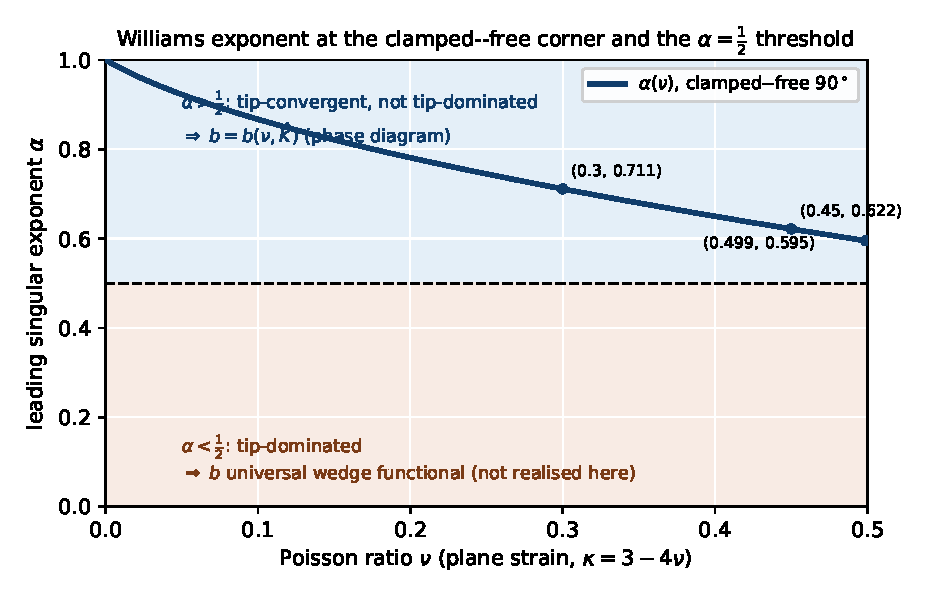
\includegraphics[width=0.72\textwidth]{figures/williams_exponent.pdf}
    \caption{Leading Williams singular exponent $\alpha(\nu)$ for the right-angle clamped--free (Dirichlet--Neumann)
        wedge (plane strain, $\kappa=3-4\nu$), the smallest root in $(0,1)$ of the $4\times4$ secular determinant of
        Proposition~\ref{prop:bcount}. Across the entire physical range the curve lies in the regime
        $\alpha>\tfrac12$ (upper band), where the cubic integral \eqref{eq:bcount} is tip-convergent but not
        tip-dominated, so the reduced coefficient retains its dependence on the normalised stress-intensity,
        $b=b(\nu,\hat K)$. The lower band $\alpha<\tfrac12$ (tip-dominated, $b$ a universal wedge functional) is not
        reached by this geometry. The exponent rises to $\alpha\to1$ as $\nu\to0$, i.e.\ the singularity \emph{weakens}
        for small Poisson ratio and the stress concentration disappears in the limit ($\bm{F}$ bounded for
        $\alpha\ge1$); this is expected, the corner stress singularity being driven by the volumetric coupling that
        vanishes as $\nu\to0$. Reproduced by \texttt{williams\_clampedfree.py} / \texttt{plot\_williams\_exponent.py}.}
    \label{fig:williams}
\end{figure}

\begin{proof}
    The scaling \eqref{eq:bcount} is immediate from $d_\phi=\det\Grad\bm{\phi}=\mathcal{O}(r^{2(\alpha-1)})$ and the
    area element $r\,dr\,d\theta$; convergence at $r=0$ is the elementary condition $4\alpha-3>-1$. The factor
    $f''(J_0)$ is bounded away from the collapse locus and only strengthens convergence under compression
    ($f''_{\log}>0$), so it does not change the count. The exponents in (i) are the smallest real roots in $(0,1)$ of
    the $4\times4$ boundary-condition determinant for the clamped ($u_r=u_\theta=0$ at $\theta=0$) and traction-free
    ($\sigma_{\theta\theta}=\sigma_{r\theta}=0$ at $\theta=\tfrac\pi2$) Kolosov--Muskhelishvili eigensolutions
    $\varphi=Cz^{\alpha}$, $\psi=Ez^{\alpha}$; the value $\alpha(0.3)\approx0.711$ reproduces the classical
    $90^\circ$ fixed--free corner. Statements (ii)--(iii) are the localisation/non-localisation alternative of the
    blow-up dichotomy (Remark~\ref{rem:sifparam}) applied to the convergent, respectively divergent, case of
    \eqref{eq:bcount}. \qed
\end{proof}

\begin{remark}[Two scales, and why flat creasing does not hand over the sign]
    \label{rem:twoscales}
    Case (ii) has a transparent mechanical reading. The buckling mode of Lemma~\ref{lem:biot} is a crease localised at
    an interior free-face point $P$ on the wavelength scale $1/k$, while the edge field varies on the scale $r_P$ of the
    distance from $P$ to $\Sigma$. If $1/k\ll r_P$ the crease sees a locally \emph{homogeneous} pre-stress and inherits
    the flat-surface sign $b<0$ for free; that limit is precisely the one $\alpha<\tfrac12$ would enforce, and it is
    \emph{not} the present case. For $\alpha>\tfrac12$ the surviving contribution lives at $1/k\sim r_P$, where the crease
    sits in the \emph{graded} pre-stress of the corner; the substrate gradient enters through $\hat K$ and the flat
    result no longer dictates the sign. This is the analytic origin of the ``$\mathcal{O}(1)$ geometry competition'' that
    makes $b$ the one irreducibly numerical coefficient.
\end{remark}

\begin{remark}[The flat reduction is degenerate; the corner is what makes $b$ exist]
    \label{rem:flatdegenerate}
    The phrase ``inherits the flat sign $b<0$'' in Remark~\ref{rem:twoscales} must be read with care, because the flat
    single-mode reduction is in fact \emph{singular}. The Biot surface-instability threshold of the homogeneous
    half-space is \emph{scale-free}: the secular condition is independent of the surface wavenumber $k$, so at
    $\lambda_\parallel=\lambda_\star$ \emph{every} harmonic is simultaneously neutral. The Lyapunov--Schmidt reduction of
    a single mode of wavenumber $k$ then feeds, at second order, a response at wavenumber $2k$ --- which is itself a
    neutral mode of the same operator. The second-harmonic problem is therefore \emph{resonant}, the orthogonal-mode
    field $\bm\psi$ does not exist as a bounded correction, and the single-mode cubic coefficient $b$ is undefined for the
    flat surface. (Numerically, the smallest singular value of the incremental operator at $\lambda_\star$ is at machine
    level for $k=1,2,3,4$ alike.) This is the precise analytic reason that flat creasing is a \emph{localised},
    finite-amplitude instability rather than a sinusoidal supercritical/subcritical bifurcation
    \cite{Hong2009}: there is no single-mode normal form to carry a sign.

    The corner removes exactly this degeneracy. The pre-stress is graded along the free face on the scale $r_P$
    (Remark~\ref{rem:twoscales}), which breaks the translational/scale invariance, couples the wavenumbers, and selects a
    \emph{discrete} critical mode --- the attainment of Lemma~\ref{lem:attain} under (BC). With the spectrum discrete and
    simple, the second-harmonic operator is no longer resonant, $\bm\psi$ exists, and $b=b(\nu,\hat K)$ is a well-defined
    number. Thus the corner is not merely the setting in which $b$ happens to be computed: it is what makes the reduced
    cubic \emph{exist} at all. This sharpens Proposition~\ref{prop:bcount} --- $b$ cannot be a bare-wedge, $\hat
        K$-independent constant, because the $\hat K\to0$ (flat) limit is not a regular point of the reduction but the
    degenerate one.
\end{remark}

The degeneracy just described is not only an obstruction; combined with the feedback-sign
Lemma~\ref{lem:fbsign}, it is a \emph{mechanism}. Near the flat limit the second harmonic is nearly neutral, so the
denominator of the certification criterion \eqref{eq:certcrit} is nearly zero --- and the feedback, which is exactly
the supremum \eqref{eq:fbvar}, is correspondingly large. This can be turned into a theorem for the small-$\hat K$
regime.

\begin{proposition}[Certified subcriticality at the edge of the flat degeneracy]
    \label{prop:certdeg}
    Let $\{(\bm{\phi}_{\hat K},\mathcal{L}_{c,\hat K})\}_{\hat K>0}$ be the family of critical states of the graded
    reduction (Proposition~\ref{prop:bcount}(ii)), and for each $\hat K$ let $\bm{v}_{\hat K}\in V^\perp$ be an
    admissible comparison field --- the natural candidate is the doubled-wavenumber surface harmonic, which by
    Remark~\ref{rem:flatdegenerate} goes neutral in the flat limit. With $E_3$ and $b_{\mathrm{dir}}$ as in
    Lemma~\ref{lem:fbsign}, set the (scaling-invariant in both $\bm\phi$ and $\bm v$) certification ratio
    \begin{equation}
        \label{eq:gammadef}
        \Gamma(\hat K) := \frac{E_3[\bm{\phi}_{\hat K},\bm{\phi}_{\hat K},\bm{v}_{\hat K}]^2}
        {2\,b_{\mathrm{dir}}(\hat K)\,\langle\bm{v}_{\hat K},\mathcal{L}_{c,\hat K}\bm{v}_{\hat K}\rangle}\ ,
    \end{equation}
    so that, by Corollary~\ref{cor:cert}, $b\le b_{\mathrm{dir}}\,(1-\Gamma)$ and $b(\nu,\hat K)<0$ whenever
    $\Gamma(\hat K)>1$. Suppose that, as $\hat K\to0^+$,
    \begin{enumerate}
        \item[\textup{(a)}] the comparison field goes neutral,
              $\langle\bm{v},\mathcal{L}_c\bm{v}\rangle/\|\bm{v}\|_V^2\to0$ (the flat resonance of
              Remark~\ref{rem:flatdegenerate}); and
        \item[\textup{(b)}] the second-harmonic coupling does not degenerate along with it:
              $E_3[\bm{\phi},\bm{\phi},\bm{v}]^2/\big(b_{\mathrm{dir}}\,\|\bm{v}\|_V^2\big)\ \ge\ c_0>0$ uniformly in
              $\hat K$.
    \end{enumerate}
    Then $\Gamma(\hat K)\to\infty$; in particular there is $\hat K_0>0$ such that $b(\nu,\hat K)<0$ for all
    $\hat K\in(0,\hat K_0)$, with diverging margin, $b_\psi/b_{\mathrm{dir}}\le-\Gamma\to-\infty$.
\end{proposition}

\begin{proof}
    Immediate from Corollary~\ref{cor:cert}:
    $\Gamma=\big[E_3^2/(b_{\mathrm{dir}}\|\bm{v}\|_V^2)\big]\cdot
        \big[2\langle\bm{v},\mathcal{L}_c\bm{v}\rangle/\|\bm{v}\|_V^2\big]^{-1}
        \ge \tfrac12\,c_0\,\big[\langle\bm{v},\mathcal{L}_c\bm{v}\rangle/\|\bm{v}\|_V^2\big]^{-1}\to\infty$
    by (a)--(b), and $b\le b_{\mathrm{dir}}(1-\Gamma)$ with $b_{\mathrm{dir}}>0$. \qed
\end{proof}

\begin{remark}[Reading, and the computational route it recommends]
    \label{rem:certnum}
    Proposition~\ref{prop:certdeg} replaces the loose analogy ``flat creasing is subcritical, so the corner should
    be'' by a statement internal to the corner: the closer the graded state sits to the degenerate flat limit, the
    more violently subcritical it is, \emph{provided} the quadratic self-coupling of the critical mode into the second
    harmonic survives the limit --- hypothesis (b), which is precisely the non-vanishing of the quantity whose
    resonance makes the flat $b$ undefined (Remark~\ref{rem:flatdegenerate}). The proposition covers the
    small-$\hat K$ regime only; on the finite $(\nu,\hat K)$ rectangle the criterion $\Gamma>1$ must still be checked.
    But it also dictates \emph{how} to check it: $\Gamma$ is assembled from one trilinear integral and one Rayleigh
    quotient, with no bordered solve, so it stays well-conditioned exactly where the direct Lyapunov--Schmidt assembly
    degrades (the near-resonant regime in which the condition number of the reduced solve diverges). We therefore
    regard \eqref{eq:certcrit}, evaluated on the computed pair $(\bm{\phi},\bm{v})$, as the proper numerical arbiter
    of the cubic clause of Assumption~\ref{ass:subcrit}, in preference to a converged value of $b$ itself.
\end{remark}

\subsection{Kinematic relief}
\label{sub:reliefd}

The kinematic relief is dimension-independent, and --- in contrast to the original formulation --- it does not require
the critical mode to be \emph{exactly} volume-preserving at first order. Earlier drafts \emph{posited}
$\operatorname{cof}\bm{F}_0:\Grad\bm{\phi}=0$; that exact condition is replaced by the weaker asymptotic smallness
$D_1=\operatorname{cof}\bm{F}_0:\Grad\bm{\phi}=\mathcal{O}(J_0/\sqrt{|\log J_0|})$ of Assumption~\ref{ass:rot} ---
small with $J_0$, but not zero. We are careful about its status: at the bifurcation $J_0(t_c)>0$ and the second
variation \eqref{eq:secondvar} is a regular form, so the smallness is automatic (Lemma~\ref{lem:rotreg}); along the
near-collapse continuation it is a hypothesis, \emph{not} derivable by isolating $f''(J)(\delta J)^2$ (the determinant
term in \eqref{eq:secondvar} is in fact more singular and numerically dominant, Remark~\ref{rem:rotnum}), and is
verified directly on the computed mode (rotation defect $\approx0.08$--$0.16$). Granting it, Lemma~\ref{lem:relief}
gives the lower bound
\begin{equation}
    \label{eq:reliefd}
    J=J_0+w\,D_1+w^2 d_\phi+\mathcal{O}(w^3) \ \ge\ \tfrac12 J_0+\tfrac12 w^2 d_\phi
    \qquad\text{in } \mathbb{R}^d,
\end{equation}
with $d_\phi$ the second mixed discriminant of $\bm{F}_0$ and $\Grad\bm{\phi}$ (the second-order coefficient of the
determinant, $=\det\Grad\bm{\phi}$ for $d=2$). The relief mechanism itself is valid for all $d$ once
Assumption~\ref{ass:rot} is granted, so it is a kinematic statement in every dimension rather than a special
two-dimensional accident. The relief floor requires the \emph{orientation} of this second-order coefficient, but --- and this is the precise
content of the localisation --- only \emph{where the relief term is actually invoked}, namely on a neighbourhood of the
collapse locus $\Sigma_{\mathrm{c}}$ (the tube where $\lambda_{\min}\to0$); off $\Sigma_{\mathrm{c}}$, where $J_0$ stays
bounded below, the sign of $d_\phi$ is immaterial (the finite-$J_0$ case~(i) of Lemma~\ref{lem:relief} absorbs a negative
$w^2 d_\phi$ into the $J_0$ margin). The localised orientation condition is
\begin{equation}
    \label{eq:dphisign}
    d_\phi\ \ge\ c_d\ >\ 0 \qquad\text{a.e.\ on a neighbourhood of $\Sigma_{\mathrm{c}}$ (the relief-orienting sign of the mode, with a uniform floor $c_d$),}
\end{equation}
which we record as a genericity property of the critical mode, \emph{not} as a consequence of
Lemma~\ref{lem:sval} (that lemma concerns the transversal vanishing of $\lambda_{\min}$, a different field). The
condition is local for a structural reason made exact by the planar identity, valid pointwise for any $\Grad\bm\phi$,
\begin{equation}
    \label{eq:dphisplit}
    d_\phi=\det\Grad\bm\phi=\det\bm E+\omega^2,\qquad
    \bm E=\tfrac12(\Grad\bm\phi+\Grad\bm\phi^{T}),\quad \omega=\tfrac12(\partial_1\phi_2-\partial_2\phi_1),
\end{equation}
(the strain/spin split; the cross term vanishes because $\bm E$ is symmetric). Thus $d_\phi>0\iff\omega^2>|\det\bm E|$:
the relief orientation is \emph{exactly} the statement that the local spin dominates the strain determinant --- the same
rotation-dominance that underlies the asymptotic-rotation mechanism \eqref{eq:rotrate}, and the reason the relief is
second order. Two consequences follow. First, $d_\phi$ is the Jacobian determinant of an \emph{oscillatory} mode, so it
flips sign cell-to-cell and a \emph{global} one-sign claim on $B_\rho$ would be generically false --- on the computed
mode of \S\ref{sec:numerical} the global positive fraction is only ${\approx}25$--$36\%$; what the lemma needs, and all
it needs, is $d_\phi>0$ where $\lambda_{\min}\to0$. Second, \eqref{eq:dphisplit} makes the numerical test sharp, and we
report its outcome honestly. Where the mode concentrates the spin dominates by ${\sim}2.4{:}1$ ($d_\phi>0$ on the
$|\Grad\bm\phi|^2$-weighted measure at ${\approx}70$--$74\%$, rising to ${\approx}80\%$ on the sub-surface annulus
carrying most modal energy), so on the bulk of the active mode the orientation is the relieving one. But the mode peaks
within a thin surface skin that coincides with the deepest compression, and \emph{there} the strain is shear-dominated,
$\det\bm E<0$ with $\omega^2/|\det\bm E|\approx0.6<1$, so $d_\phi<0$ on the deepest-$J_0$ decile. In the computable
range this skin is harmless --- the base states keep $J_0\gtrsim0.5$, so $\lambda_c=\lambda_{\min}(\bm F_0)$ is bounded
below and the finite-$J_0$ case~(i) of Lemma~\ref{lem:relief} absorbs the negative $w^2 d_\phi$ with no sign hypothesis
(this part is \emph{proved}, not assumed). The relief floor $C_2 w^2$ is invoked only in the genuine collapse limit
$J_0\to0$ along the unstable continuation, which the barrier $f''_{\log}\sim|\log J_0|/J_0^2$ puts beyond reach of the
solver; a mode-following deepening sweep toward it finds the deep-skin ratio $\omega^2/|\det\bm E|$ \emph{drifting
slightly downward} ($0.65\to0.61$), so the accessible evidence does not support $d_\phi>0$ at $\Sigma_{\mathrm{c}}$ and,
if anything, leans against it. We therefore keep \eqref{eq:dphisign} as a genuine hypothesis on the same footing as the
rate \eqref{eq:rotrate} --- needed only in the unreachable limit, neither verified nor, on present evidence, favoured
there --- while stressing that the regularisation everywhere the computation reaches is independent of it
(Remark~\ref{rem:rotnum}). Lemma~\ref{lem:orient} below sharpens this status considerably: the orientation is
\emph{proved}, pointwise, wherever the mode is locally a quadrature surface wave with one-signed, monotonically
decaying envelopes, and the possible failure is confined to --- and characterised on --- the strain-dominated skin. The remaining
points for the concrete model are that the collapse locus $\Sigma_{\mathrm{c}}$ is
generically the
codimension-one set inside $B_\rho$ along which the relieved branch would still collapse (or, when the severest
compression sits at the vertex, the point $\Sigma_{\mathrm{c}}=\{0\}$ of codimension two, Remark~\ref{rem:locus}, which
only sharpens the integrability); the regularised bound of
Theorem~\ref{thm:reg} and the localisation of Proposition~\ref{prop:narrow} then apply verbatim.

The status of the orientation condition can be made exact rather than statistical. The following identities replace
the sampled sign fractions of \S\ref{sec:numerical} by closed-form criteria on the mode itself.

\begin{lemma}[Exact orientation identities for a surface-wave mode]
    \label{lem:orient}
    Let $d_\phi=\det\Grad\bm\phi$ in $d=2$, with components $\phi_1$ along the free face and $\phi_2$ normal to it.
    \begin{enumerate}
        \item[\textup{(i)}] \emph{(Null Lagrangian: the bulk carries no net orientation.)} For every Lipschitz
              subdomain $\omega\subset B_\rho$,
              \begin{equation}
                  \label{eq:nulllag}
                  \int_\omega d_\phi\,dV \;=\; \oint_{\partial\omega}\phi_1\,\partial_\tau\phi_2\,ds ,
              \end{equation}
              $\tau$ the positively oriented tangent. The net orientation of the mode over any cell is a boundary
              quantity; over $B_\rho$ (where $\bm\phi$ vanishes on $\Gamma_D$ and, for the localised mode, on
              $\partial B_\rho$) it is carried \emph{entirely by the free face}. In particular any global bulk
              statistic of $\operatorname{sign}(d_\phi)$ is structurally uninformative --- the rescoping of
              \eqref{eq:dphisign} to the collapse tube is forced, not merely prudent.
        \item[\textup{(ii)}] \emph{(Surface-wave mean: an exact depth derivative.)} If locally
              $\bm\phi=\mathrm{Re}\big[\bm U(n)\,e^{\mathrm{i}kx}\big]$, with $x$ the arc length along the free face
              and $n\ge0$ the depth, the average over one wavelength is
              \begin{equation}
                  \label{eq:dbar}
                  \bar d_\phi(n)=-\frac{k}{2}\,\frac{d}{dn}\,\mathrm{Im}\big(U_1\overline{U_2}\big),
                  \qquad
                  \int_0^\infty \bar d_\phi\,dn=\frac{k}{2}\,\mathrm{Im}\big(U_1\overline{U_2}\big)\Big|_{n=0}:
              \end{equation}
              the depth-integrated mean orientation is set by the relative phase of the two displacement components
              \emph{at the surface} alone, consistently with (i).
        \item[\textup{(iii)}] \emph{(Quadrature modes: pointwise sign.)} If moreover the mode is in exact quadrature,
              \begin{equation}
                  \label{eq:quadmode}
                  \phi_1=-a(n)\,\sin kx,\qquad \phi_2=b(n)\,\cos kx
              \end{equation}
              (the form of a surface-instability eigenmode with real Stroh roots and real amplitude ratios), then
              \emph{pointwise, at every} $(x,n)$,
              \begin{equation}
                  \label{eq:dpointwise}
                  d_\phi=-k\,\big[a\,b'\,\cos^2 kx+a'\,b\,\sin^2 kx\big] .
              \end{equation}
              Hence $d_\phi>0$ everywhere if and only if $a\,b'<0$ and $a'\,b<0$; in particular, if the envelopes
              $a,b$ share a common sign and both decay monotonically in depth, then $d_\phi>0$ \emph{pointwise} ---
              the orientation condition \eqref{eq:dphisign} holds with no averaging and no genericity. Conversely, a
              sign change of $\bar d_\phi$ at depth $n$ marks an interior extremum of the envelope product $ab$.
    \end{enumerate}
\end{lemma}

\begin{proof}
    (i) $\det\Grad\bm\phi=\partial_1(\phi_1\partial_2\phi_2)-\partial_2(\phi_1\partial_1\phi_2)$, the mixed second
    derivatives cancelling, i.e.\ $d_\phi=\operatorname{div}\big(\phi_1\partial_2\phi_2,\,-\phi_1\partial_1\phi_2\big)$;
    the divergence theorem and $(\partial_2\phi_2,-\partial_1\phi_2)\cdot\bm{n}=\partial_\tau\phi_2$ give
    \eqref{eq:nulllag}. (ii) With $\partial_x\phi_i=\mathrm{Re}[\mathrm{i}kU_ie^{\mathrm{i}kx}]$ and
    $\partial_n\phi_i=\mathrm{Re}[U_i'e^{\mathrm{i}kx}]$, the product formula
    $\mathrm{Re}[Ae^{\mathrm{i}kx}]\,\mathrm{Re}[Be^{\mathrm{i}kx}]
        =\tfrac12\mathrm{Re}[A\bar B]+\tfrac12\mathrm{Re}[ABe^{2\mathrm{i}kx}]$ yields
    $\bar d_\phi=\tfrac12\mathrm{Re}\big[\mathrm{i}k\,(U_1\bar U_2'+U_1'\bar U_2)\big]
        =\tfrac12\mathrm{Re}\big[\mathrm{i}k\,(U_1\bar U_2)'\big]$, which is \eqref{eq:dbar}; the integral follows from
    the decay at $n=\infty$. (iii) Direct differentiation of \eqref{eq:quadmode} gives
    $d_\phi=(-ka\cos kx)(b'\cos kx)-(-a'\sin kx)(-kb\sin kx)$, which is \eqref{eq:dpointwise}; its mean
    $-\tfrac k2(ab)'$ agrees with \eqref{eq:dbar} at $U_1=\mathrm{i}a$, $U_2=b$. \qed
\end{proof}

\begin{remark}[What the identities change]
    \label{rem:orient}
    Three consequences. \emph{First}, the localisation of \eqref{eq:dphisign} is structural: by \eqref{eq:nulllag}
    the Jacobian of the mode has no bulk mass, so a global one-sign claim was never the right invariant. \emph{Second},
    on the bulk of the active mode the orientation is now \emph{proved}, not sampled: where the computed mode is
    locally a decaying quadrature surface wave with one-signed envelopes --- the sub-surface annulus carrying most of
    the modal energy --- Lemma~\ref{lem:orient}(iii) gives $d_\phi>0$ pointwise, in agreement with the
    ${\approx}70$--$80\%$ weighted fractions of \S\ref{sec:numerical} (the shortfall from $100\%$ measures exactly the
    extent to which the grading modulates the envelope in $x$ and breaks exact quadrature). \emph{Third}, the possible
    failure of \eqref{eq:dphisign} is localised and characterised: it can occur only where an envelope is
    non-monotone or changes sign --- for the computed eigenmode, the thin strain-dominated skin above the envelope
    extremum, where the observed $\omega^2/|\det\bm E|\approx0.6$ sits. The open content of \eqref{eq:dphisign} is
    thereby reduced from a genericity postulate on $\bm\phi$ to a single explicit question: whether, in the collapse
    limit $J_0\to0$, the envelope extremum of the critical mode detaches from the collapse tube (relief holds) or
    rides on it (relief fails). That question is posed on the Stroh data of the compressible surface eigenmode ---
    two exponents and two amplitude ratios fixed by the secular condition --- and is answerable in closed form; we
    leave its evaluation to the planned wedge computation.
\end{remark}

\subsection{Attainment of the critical mode}
\label{sub:attain}

The second half of Assumption~\ref{ass:bif} --- that $\mu_1(t_c)=0$ is \emph{attained} by a genuine eigenmode rather
than being the bottom of essential spectrum --- looks like the hard, borderline-elliptic point of
Remark~\ref{rem:framework}. It is in fact a consequence of a single, transparent geometric condition: that the
\emph{buckling precedes the pointwise collapse} of the fundamental state. The essential-spectrum threat is tied to the
scale-invariance of the corner at collapse (the same wavenumber degeneracy that makes flat creasing scale-free, and
that let $k\to\infty$ in Lemma~\ref{lem:biot}); it is activated only when $\mathbb{L}$ blows up, i.e. only when
$\lambda_{\min}\to0$. So long as the crossing occurs while the fundamental stretch is still bounded below, the operator
has bounded coefficients and the spectrum is discrete.

\begin{assumption}[Buckling precedes collapse, (BC)]
    \label{ass:bc}
    The fundamental path keeps the stretch off collapse up to the crossing:
    \begin{equation}
        \label{eq:bc}
        \inf_{t\le t_c}\ \inf_{\bm{x}\in\overline{B_\rho}}\ \lambda_{\min}\big(\bm{F}_0(t,\bm{x})\big)\ \ge\ c>0 .
    \end{equation}
\end{assumption}

\begin{lemma}[Attainment under (BC)]
    \label{lem:attain}
    Assume, in addition to \textup{(BC)}, that the fundamental state $(t,\bm x)\mapsto\bm F_0(t,\bm x)$ is continuous on
    the compact cylinder $[0,t_c]\times\overline{B_\rho}$ --- a standing regularity of the load path, automatic for a
    fundamental branch depending continuously on the load with bounded data. Then for every $t\le t_c$ the tangent
    $\mathbb{L}(\bm{F}_0(t))$ is bounded on $B_\rho$, the
    operator $\mathcal{L}_c=\partial_{\bm{u}}G(\bm{u}_0(t_c),t_c,0)$ has compact resolvent and discrete spectrum, and the
    critical value $\mu_1(t_c)=0$ is attained by an eigenmode $\bm{\phi}\in V$. This discharges the
    \emph{attainment} clause of Assumption~\ref{ass:bif}; the \emph{simplicity} clause is reduced, by the symmetry
    argument of \S\ref{sub:symmetry}, to the generic statement that the lowest eigenvalue \emph{within} the symmetry
    sector carrying $\bm{\phi}$ is simple.
\end{lemma}

\begin{proof}
    Condition \eqref{eq:bc} supplies the \emph{lower} stretch bound, $\|\bm{F}_0(t)^{-1}\|=\lambda_{\min}^{-1}\le
        c^{-1}$. The matching \emph{upper} bound is not part of (BC) --- which constrains only $\lambda_{\min}$ --- but follows
    from the stated continuity hypothesis: $(t,\bm x)\mapsto\bm F_0(t,\bm x)$ is continuous on the compact set
    $[0,t_c]\times\overline{B_\rho}$, so all
    its stretches, and in particular $\det\bm F_0$, are bounded above by a constant $C_0=C_0(t_c)<\infty$ there.
    Together with $\Theta_{\log}$ being continuous and finite on the compact range $[\,(\det\bm F_0)_{\min},C_0\,]$
    (which avoids $J=0$ by (BC)), the structural bound \eqref{eq:Lbound},
    $\|\mathbb{L}(\bm{F}_0(t))\|\le\mu_e+c^{-2}\Theta_{\log}(\det\bm{F}_0)$, is uniformly bounded on $B_\rho$ for
    $t\le t_c$. By Lemma~\ref{lem:SEcompress} the same tensor is strongly elliptic with constant $\ge\mu_e$ throughout
    compression; with Korn's inequality the second-variation form obeys a G\aa rding estimate
    $Q_{t_c}(\bm{v})\ge\gamma\,\|\bm{v}\|_{H^1(B_\rho)}^2-C\,\|\bm{v}\|_{L^2(B_\rho)}^2$ on $V\subset H^1$. Thus
    $\mathcal{L}_c+C$ is coercive on $H^1$, its inverse maps $L^2$ boundedly into $H^1$, and the Rellich embedding
    $H^1(B_\rho)\hookrightarrow\hookrightarrow L^2(B_\rho)$ --- valid on the bounded domain, the edge $\Sigma$
    notwithstanding --- makes the resolvent of $\mathcal{L}_c$ compact. A self-adjoint operator with compact resolvent
    has purely discrete spectrum and attains its lowest eigenvalue; at $t_c$ that eigenvalue is $\mu_1(t_c)=0$, with
    eigenmode $\bm{\phi}$. \qed
\end{proof}

\begin{remark}[What (BC) costs, and why it is the right residue]
    \label{rem:bc}
    Lemma~\ref{lem:attain} relocates the difficulty from a functional-analytic statement about essential spectrum to a
    comparison of two load thresholds: the buckling load $t_c$ and the pointwise-collapse load
    $t_{\mathrm{coll}}:=\inf\{t:\inf_{B_\rho}\lambda_{\min}(\bm{F}_0(t))=0\}$, with (BC) asking $t_c<t_{\mathrm{coll}}$.
    This is genuinely cleaner than ``attainment'': (i) Lemma~\ref{lem:biot} already bounds $t_c$ from above by the
    surface-creasing load $t_*$, attained while $\lambda_{\min}\approx\lambda_\star=\mathcal{O}(1)$ at the creasing point
    --- not at collapse; (ii) the barrier $f_{\log}(J)\to\infty$ makes $J=0$ cost infinite energy, so the true (not
    linearly-predicted) fundamental path resists pointwise collapse and pushes $t_{\mathrm{coll}}$ up; and (iii) (BC) is
    directly checkable in a computation, by monitoring $\min_{\bm{x}}\lambda_{\min}$ at the detected crossing. The one
    place it can fail is the edge tip, where the \emph{linear} prediction $\lambda_{\min}\sim1-|K|r^{\alpha-1}$ wants to
    collapse for any load; bounding the barrier-regularised tip collapse load from below is the concrete content left
    open, in place of the opaque spectral hypothesis. Lemma~\ref{lem:measrep} and Proposition~\ref{prop:tipdisc} below
    make (ii) and the tip localisation quantitative: collapse is repelled in measure at an explicit logarithmic rate
    and spatially confined to a disc whose radius is explicit in $(\hat K,\alpha)$; the residual content of (BC) is
    thereby reduced to a pointwise floor on that single shrinking disc. One further consequence of stating the path
    hypotheses up front (Assumption~\ref{ass:fp}) deserves emphasis: the floor is needed at the \emph{Biot} load
    $t_*$, not at collapse. By Lemma~\ref{lem:tc}, once $t_*<t_{\mathrm{coll}}$ --- i.e.\ once the tip disc has not
    collapsed by the load at which the free-face stretch reaches $\lambda_\star$, with the state there uniformly
    non-degenerate ($\lambda_{\min}\approx\lambda_\star=\mathcal O(1)$ at the creasing point) --- the ordering
    $t_c\le t_*<t_{\mathrm{coll}}$ is a \emph{conclusion}, not a separate hypothesis: (BC) collapses to the single
    quantitative bound $t_{\mathrm{coll}}>t_*$, checkable through \eqref{eq:scsafe}.
\end{remark}

\begin{lemma}[The barrier repels collapse in measure]
    \label{lem:measrep}
    For the energy \eqref{eq:neohooke} with $f_{\log}$ one has the pointwise coercivity
    \begin{equation}
        \label{eq:psicoerc}
        \Psi(\bm F)\ \ge\ \lambda_e\,\log^2 J \qquad \text{for all } \bm F\in\mathrm{GL}^+(2).
    \end{equation}
    Let $\bm u_0(t)$ be \emph{any} admissible branch whose energy stays below an explicit finite bound,
    $\mathcal E_t(\bm u_0(t))\le E(t)$: minimality itself is not used, only the energy bound. The global-minimiser
    branch of Lemma~\ref{lem:fundexist} qualifies by construction under displacement control, with
    $E(t):=\mathcal E_t(\bm u_{\mathrm{trial}})$ for any fixed admissible competitor (finite and explicit for the
    bodies (H), (C), e.g.\ the smooth ramp extension of the boundary data); so does any stable or unstable
    continuation --- past $t_c$ included --- on which the energy is monitored and found below $E(t)$. Then for
    every $\delta\in(0,1)$,
    \begin{equation}
        \label{eq:measrep}
        \big|\{\bm x\in B_\rho:\ J_0(t,\bm x)\le\delta\}\big|\ \le\ \frac{E(t)}{\lambda_e\,\log^2\delta}\ .
    \end{equation}
    In particular the sublevel sets of $J_0$ shrink at an explicit logarithmic rate: a collapse tube
    $\{J_0\le\delta\}$ around a codimension-one locus $\Sigma_{\mathrm{c}}$ of length $|\Sigma_{\mathrm{c}}|$ has mean
    half-width $\le E(t)/\big(2\lambda_e|\Sigma_{\mathrm{c}}|\log^2\delta\big)$, and pointwise collapse ($J_0=0$) can
    occur at most on a null set at any finite load. The same holds under traction loading whenever the load
    functional stays bounded along the path, with $E(t)$ replaced by
    $E(t)+\sup_{s\le t}|\ell_s(\bm u_0(s))|$.
\end{lemma}

\begin{proof}
    In $d=2$, writing the principal stretches $\lambda_i$ and using $\tr(\bm F^T\bm F)=\sum_i\lambda_i^2$,
    $\log J=\sum_i\log\lambda_i$,
    \begin{equation*}
        \Psi(\bm F)=\sum_{i}\tfrac{\mu_e}{2}\big(\lambda_i^2-1-\log\lambda_i^2\big)\;+\;\lambda_e\log^2 J
        \ \ge\ \lambda_e\log^2 J,
    \end{equation*}
    since $s-1-\log s\ge0$ at $s=\lambda_i^2$; this is \eqref{eq:psicoerc}. By the assumed energy bound
    $\int_{B_\rho}\lambda_e\log^2J_0\,dV\le\mathcal E_t(\bm u_0(t))\le E(t)$, and Chebyshev's inequality on
    $\{J_0\le\delta\}$, where $\log^2J_0\ge\log^2\delta$, gives \eqref{eq:measrep}. \qed
\end{proof}

\begin{proposition}[Collapse, if anywhere, is confined to the tip disc]
    \label{prop:tipdisc}
    Along the fundamental path, for $t<t_{\mathrm{coll}}$, assume the corner expansion of hypothesis (FP)(ii) ---
    the Kondratiev form of Proposition~\ref{prop:blowup}(i) with pointwise gradient control of the remainder,
    $|\Grad\bm u_0^\sharp|\le C_\sharp(t)\,(r/\rho)^{\alpha'-1}$; this is a genuine hypothesis on the nonlinear
    state, not a citation, since the linear theory \cite{KMR2001,MazyaRossmann2010} attaches to it only through a
    frozen-coefficient reading and, under compression, no screening mechanism pins the vertex behaviour
    (Remark~\ref{rem:fp}). Set
    $c_\Phi:=\max_\theta\big\|\alpha\,\bm\Phi\otimes\bm e_r+\bm\Phi'\otimes\bm e_\theta\big\|$, so that the leading
    term obeys $\big\|\Grad\big(K r^\alpha\bm\Phi\big)\big\|\le c_\Phi\,\mu_e\,|\hat K(t)|\,(r/\rho)^{\alpha-1}$ by
    the normalisation $\hat K=K\rho^{\alpha-1}/\mu_e$ of Remark~\ref{rem:sifparam}. With
    $M(t):=c_\Phi\,\mu_e\,|\hat K(t)|+C_\sharp(t)$ bounded along the path,
    \begin{equation}
        \label{eq:tipfloor}
        \lambda_{\min}\big(\bm F_0(t,\bm x)\big)\ \ge\ 1-M(t)\,\Big(\frac{r}{\rho}\Big)^{\alpha-1},
        \qquad \bm x\in B_\rho ,
    \end{equation}
    so $\lambda_{\min}\ge\tfrac12$ everywhere outside the \emph{tip disc}
    \begin{equation}
        \label{eq:tipradius}
        r\ \le\ r_0(t):=\rho\,\big(2M(t)\big)^{\frac{1}{1-\alpha}} .
    \end{equation}
    Consequently:
    \begin{enumerate}
        \item[\textup{(i)}] letting $t\uparrow t_{\mathrm{coll}}$, any collapse point lies in the closed disc
              $\{r\le r_0(t_{\mathrm{coll}})\}$: condition (BC) can fail \emph{only through the tip}, the assertion of
              Remark~\ref{rem:bc} upgraded from a heuristic to an estimate, with the failure region quantified by the
              computable pair $(\hat K,\alpha)$;
        \item[\textup{(ii)}] the surface-instability point $P$ of (SC), at fixed distance $r_P$ from $\Sigma$, is
              provably not the collapse site whenever $r_0(t_*)<r_P$, i.e.\ whenever
              \begin{equation}
                  \label{eq:scsafe}
                  M(t_*) \ <\ \tfrac12\,\Big(\frac{r_P}{\rho}\Big)^{1-\alpha},
              \end{equation}
              an explicit inequality between computable numbers; granted \eqref{eq:scsafe}, the destabilising field of
              Lemma~\ref{lem:biot} lives entirely in the region where \eqref{eq:tipfloor} keeps the state uniformly
              non-degenerate, and the ordering $t_c<t_{\mathrm{coll}}$ can fail only if the tip disc
              \eqref{eq:tipradius} collapses before the free-face stretch reaches $\lambda_\star$;
        \item[\textup{(iii)}] combined with Lemma~\ref{lem:measrep} the two smallness mechanisms compound: the
              possible collapse set is contained in a disc of radius $r_0$ \emph{and} has measure
              $\mathcal O\big(E(t)/\log^2\delta\big)$ at depth $\delta$.
    \end{enumerate}
\end{proposition}

\begin{proof}
    For $t<t_{\mathrm{coll}}$ the state is uniformly non-degenerate on $\overline{B_\rho}$ by (FP)(i) and the
    coefficients are bounded (Lemma~\ref{lem:attain}); the expansion
    $\bm u_0=K r^\alpha\bm\Phi(\theta)+\bm u_0^\sharp$ holds with the stated bounds by hypothesis (FP)(ii). Then
    $\Grad\bm u_0=K r^{\alpha-1}\big(\alpha\,\bm\Phi\otimes\bm e_r+\bm\Phi'\otimes\bm e_\theta\big)+\Grad\bm u_0^\sharp$
    and, by Weyl's inequality for singular values,
    $\lambda_{\min}(\bm I+\Grad\bm u_0)\ge1-\|\Grad\bm u_0\|$, which with
    $(r/\rho)^{\alpha'-1}\le(r/\rho)^{\alpha-1}$ on $r\le\rho$ (recall $\alpha'>\alpha$) gives \eqref{eq:tipfloor}.
    The right-hand side of \eqref{eq:tipfloor} is $\ge\tfrac12$ iff $r\ge r_0(t)$, giving the dichotomy; (i) follows
    by continuity of $\lambda_{\min}$ in $t$ up to the first failure, (ii) by inserting $t=t_*$ and
    Lemma~\ref{lem:biot}, (iii) by intersecting with \eqref{eq:measrep}. \qed
\end{proof}

\begin{lemma}[\textup{(BC)} reduces to a comparison of wedge \emph{stretch} thresholds]
    \label{lem:bcwedge}
    The two thresholds that (BC) compares are \emph{stretch} values, and as such are scale-invariant data of the model
    wedge $\mathcal{L}_W$ of Proposition~\ref{prop:blowup}, depending on the geometry only through $\nu$ and free of the
    stress-intensity amplitude $\hat K$: the surface-instability stretch $\lambda_\star=\lambda_\star(\nu)\in(0,1)$ at
    which buckling is triggered, and the collapse stretch $\lambda_{\min}=0$. The conversion of these stretch thresholds
    into the load ordering $t_c<t_{\mathrm{coll}}$ is \emph{not} itself a wedge statement: it requires the fundamental
    state's load-to-stretch map $t\mapsto\lambda_\parallel(\bm F_0(t);P)$, a global datum. Under monotone compression
    (condition \textup{(M)} of Lemma~\ref{lem:transversal}) this map is monotone, so the stretch ordering
    $\lambda_\star>0$ transfers to the load ordering, \emph{provided} the barrier-regularised collapse load
    $t_{\mathrm{coll}}$ admits the lower bound left open in Remark~\ref{rem:bc}.
\end{lemma}

\begin{proof}
    What localises to the wedge is the pair of \emph{stretch} thresholds. The surface-instability stretch
    $\lambda_\star$ and the Biot secular form $q(\lambda_\parallel)$ are functions of $\nu$ alone
    (Remark~\ref{rem:threshold}), evaluated on the half-space tangent to the free face --- a sub-object of
    $\mathcal{L}_W$; the collapse stretch is the universal value $\lambda_{\min}=0$. Both are amplitude-free.
    Lemma~\ref{lem:biot} shows that once the fundamental state drives $\lambda_\parallel$ below $\lambda_\star$ at some
    free-face point, a destabilising field exists, hence $t_c\le t_*$ where $t_*$ is the load realising
    $\lambda_\parallel=\lambda_\star$. This load $t_*$ is \emph{not} a wedge quantity: it is the value of the global
    map $t\mapsto\lambda_\parallel(\bm F_0(t);P)$ at the threshold stretch, and that map is set by the fundamental
    state, not by the half-space model. The earlier draft conflated the (wedge) threshold stretch with the (global)
    threshold load; we separate them here. The load \emph{ordering} $t_c<t_{\mathrm{coll}}$ is what (BC) needs, and it
    follows once two genuinely non-wedge facts are granted: (a) under monotone compression (M) the map
    $t\mapsto\lambda_\parallel$ (resp.\ $\lambda_{\min}$) is monotone decreasing, so the stretch ordering
    $\lambda_\star>0=\lambda_{\min}^{\mathrm{coll}}$ converts to $t_*\le t_{\mathrm{coll}}$; and (b) the
    barrier-regularised $t_{\mathrm{coll}}$ is bounded below at the tip, the open content of Remark~\ref{rem:bc}. What
    the wedge reduction \emph{does} deliver, free of $\hat K$, is that the thresholds being compared are amplitude-free,
    $\nu$-only stretches; the amplitude $\hat K$ and the finite body enter only through the load-to-stretch map and
    through the $\mathcal{O}(\lambda^{g})$ corrections of Proposition~\ref{prop:blowup}(ii). \qed
\end{proof}

\begin{remark}[Why (BC) localises but the cubic sign need not]
    \label{rem:bclocalises}
    Lemma~\ref{lem:bcwedge} is the easy half of the localisation programme: the \emph{stretch thresholds} being
    compared ($\lambda_\star$ and $0$) are amplitude-free, $\nu$-only wedge data, decided by a single computation
    independent of (H) versus (C); the only non-wedge ingredient is the monotone load-to-stretch map that turns the
    stretch comparison into a load ordering. The subcritical \emph{sign} of \S\ref{sub:bcount} is
    the hard half: there the relevant object is an integral, not a threshold, and whether it localises is governed by the
    homogeneity count of Proposition~\ref{prop:bcount}. The two open conditions thus sit on opposite sides of the
    blow-up dichotomy of Remark~\ref{rem:sifparam}.
\end{remark}

\subsection{The irreducible core}
\label{sub:core}

Table~\ref{tab:status} summarises the effect of fixing the concrete model. Of the hypotheses of
\S\ref{sec:asymptotics}--\S\ref{sec:iba}, the material assumptions are discharged by the neo-Hookean structure
(\S\ref{sub:tier1}), the existence of the critical load by the localized-creasing Lemma~\ref{lem:biot} under the
loading hypothesis (SC), mode simplicity and the vanishing quadratic by reflection symmetry (\S\ref{sub:symmetry}), and
mode attainment by Lemma~\ref{lem:attain} under the geometric condition (BC). What remains are two hypotheses, both now
in concrete, checkable form rather than as opaque spectral postulates:
\begin{enumerate}
    \item \emph{Buckling precedes collapse}, (BC) (Assumption~\ref{ass:bc}): the threshold inequality
          $t_c<t_{\mathrm{coll}}$ that powers attainment (Lemma~\ref{lem:attain}). It is bounded on one side by
          Lemma~\ref{lem:biot} ($t_c\le t_*$, at $\lambda_{\min}=\mathcal{O}(1)$) and supported by the energy barrier
          (Remark~\ref{rem:bc}), now quantitatively: collapse is repelled in measure at an explicit logarithmic rate
          (Lemma~\ref{lem:measrep}) and spatially confined to the tip disc of radius
          $r_0\sim\rho\,(2M)^{1/(1-\alpha)}$ (Proposition~\ref{prop:tipdisc}), so the residual content is a pointwise
          floor on that single shrinking disc, which we verify numerically. By Lemma~\ref{lem:bcwedge} the two
          \emph{stretch} thresholds being compared are amplitude-free, one-parameter ($\nu$) wedge data, independent
          of the body and of $\hat K$; the conversion to the load ordering uses only the monotone load-to-stretch map
          of the fundamental state (condition (M)).
    \item \emph{Subcritical sign pattern}, $b<0<d$ (Assumption~\ref{ass:subcrit}): the directions in which the cubic and
          quintic bend the branch. Here the neo-Hookean structure is doubly informative. Lemma~\ref{lem:volcoeff}
          reduces the coefficients to volumetric integrals and shows the explicit single-mode parts are \emph{adverse}
          to subcriticality ($b_{\mathrm{dir}}>0$, $d_{\mathrm{dir}}<0$ in compression), so $b<0<d$ can come only from
          the geometry-dependent orthogonal-mode feedback. For the cubic, the \emph{direction} of that feedback is now
          a theorem, $b_\psi\le0$ (Lemma~\ref{lem:fbsign}), so the open content is the magnitude comparison
          $|b_\psi|>b_{\mathrm{dir}}$: proved for small $\hat K$ under the coupling non-degeneracy of
          Proposition~\ref{prop:certdeg}, and on the finite rectangle certifiable by the inversion-free criterion of
          Corollary~\ref{cor:cert}, which we evaluate numerically (Remarks~\ref{rem:bsign}, \ref{rem:certnum}). The
          homogeneity count of Proposition~\ref{prop:bcount} pins down \emph{why} the magnitude is irreducible:
          because the edge exponent satisfies $\alpha>\tfrac12$ here, the cubic integral is tip-convergent but not
          tip-dominated, so $b$ does not collapse to a universal wedge number but remains a functional $b(\nu,\hat K)$
          of the Poisson ratio and the normalised stress-intensity --- the quantity the computation maps out.
\end{enumerate}

\begin{table}[t]
    \centering
    \begin{tabular}{lll}
        \toprule
        Hypothesis                                                                & Abstract status                                                & Status for the concrete model                                                                                   \\
        \midrule
        Reg./growth/ellip./mild (Ass.~\ref{ass:reg}--\ref{ass:mild})              & standing assumptions                                           & \textbf{proved} (Lem.~\ref{lem:nh}, \S\ref{sub:tier1})                                                          \\
        Edge exponent $\alpha$, scenario selection                                & abstract pencil                                                & \textbf{computed} $\alpha(\nu){\in}(0.6,0.87)$; B by $K{<}0$ (\S\ref{sub:edgeexp})                              \\
        Localisation to model wedge                                               & informal                                                       & \textbf{proved}: blow-up reduction (Prop.~\ref{prop:blowup})                                                    \\
        Critical load $t_c$ exists (Lem.~\ref{lem:tc}(ii))                        & not established                                                & \textbf{proved} under (SC) (Lem.~\ref{lem:biot})                                                                \\
        Transversality (M) (Lem.~\ref{lem:transversal})                           & input on loading                                               & \textbf{holds} for monotone compression                                                                         \\
        Mode simplicity (Ass.~\ref{ass:bif})                                      & assumed                                                        & \textbf{generic} in $(\nu,\hat K)$ per symmetry sector (\S\ref{sub:symmetry}); gap checked numerically          \\
        Quadratic coeff.\ vanishes (Ass.~\ref{ass:subcrit})                       & assumed by symmetry                                            & \textbf{proved}: $c_2$ odd in $D_1$, $R$-forced (Lem.~\ref{lem:volcoeff})                                       \\
        Mode attainment (Ass.~\ref{ass:bif})                                      & assumed                                                        & \textbf{proved} under (BC) (Lem.~\ref{lem:attain})                                                              \\
        First-order relief / rotation (Ass.~\ref{ass:rot}, Lem.~\ref{lem:relief}) & finite at $t_c$ (Lem.~\ref{lem:rotreg}); near-collapse posited & \emph{numerical}: rotation defect ${\approx}0.08$--$0.16$ (Rem.~\ref{rem:rotnum})                               \\
        Stable-branch non-degeneracy (Ass.~\ref{ass:nd})                          & posited                                                        & \emph{physical} (bounded-distortion crease); not computed here (Prop.~\ref{prop:physical})                      \\
        \midrule
        Buckling precedes collapse (BC) (Ass.~\ref{ass:bc})                       & ---                                                            & \emph{numerical} on tip disc only; measure-repelled + confined (Lem.~\ref{lem:measrep}, Prop.~\ref{prop:tipdisc}, Lem.~\ref{lem:bcwedge})  \\
        Subcriticality $b<0<d$ (Ass.~\ref{ass:subcrit})                           & assumed                                                        & feedback sign \textbf{proved} $b_\psi{\le}0$ (Lem.~\ref{lem:fbsign}); magnitude \emph{numerical/certifiable} (Cor.~\ref{cor:cert}, Prop.~\ref{prop:certdeg})     \\
        \bottomrule
    \end{tabular}
    \caption{Hypothesis ledger for the concrete clamped--free neo-Hookean model. Fixing the material and geometry
        discharges every spectral postulate; the residue is two concrete, numerically checkable conditions --- that
        buckling precedes pointwise collapse, and that the reduced cubic is subcritical.}
    \label{tab:status}
\end{table}

The upshot is that for the clamped--free neo-Hookean corner under compression the abstract picture of
\S\ref{sec:asymptotics}--\S\ref{sec:iba} is, but for two clearly delimited conditions, a sequence of theorems: the
material bounds are explicit, the corner is genuinely compressive, the instability is a free-face creasing event with a
constructed destabilising field, the critical mode is attained and (generically, within its symmetry sector) simple,
with no quadratic term by symmetry, and the kinematic relief that regularises the tangent holds in every dimension once
the asymptotic-rotation hypothesis is granted. Notably, the spectral postulates of the abstract theory are sharply
reduced: attainment is \emph{proved} under (BC), and simplicity is reduced to genericity within the symmetry sector
carrying the critical mode rather than posited outright; the first-order volume preservation (rotation condition) that
the relief once posited as an exact identity is now the weaker explicit assumption (AR, \S\ref{sub:reliefd}), automatic
at the bifurcation (Lemma~\ref{lem:rotreg}) and numerically supported toward collapse rather than a barrier-forced
theorem. What remains are two \emph{concrete} and numerically checkable conditions: that buckling precedes pointwise
collapse ($t_c<t_{\mathrm{coll}}$) --- with the possible failure now confined to an explicit tip disc and repelled in
measure (Proposition~\ref{prop:tipdisc}, Lemma~\ref{lem:measrep}) --- and that the reduced cubic is subcritical
($b<0$) --- now a pure \emph{magnitude} comparison, its sign structure being settled by Lemma~\ref{lem:fbsign} and its
small-$\hat K$ regime by Proposition~\ref{prop:certdeg}. Both are exactly what the
creasing problem on a flat surface also leaves to computation, and they are inherited here rather than created by the
corner.

Finally, the blow-up reduction of \S\ref{sub:blowup} sharpens what ``numerical'' means for these two residues. By
Proposition~\ref{prop:blowup} the singularity is localised to the model wedge $\mathcal{L}_W$, all of whose data are
functions of $(\nu,\hat K)$ alone; the finite body (H) or (C) enters only through the single scalar $\hat K$ and
through corrections $\mathcal{O}(\lambda^{g})$. The two residual conditions then occupy opposite sides of a clean
homogeneity dichotomy (Remark~\ref{rem:sifparam}): condition (BC) compares two \emph{scale-invariant stretch
    thresholds}, which are one-parameter ($\nu$) wedge data on $\mathcal{L}_W$ (the conversion to a load ordering using
only the monotone load-to-stretch map, Lemma~\ref{lem:bcwedge}), whereas the cubic sign is an \emph{integral} with
$\alpha>\tfrac12$, hence tip-convergent but not tip-dominated, and remains a genuine two-parameter functional
$b(\nu,\hat K)$ (Proposition~\ref{prop:bcount}). In both cases the verification is thus a computation on a
\emph{universal} object --- a curve or a phase diagram of the corner singularity itself --- rather than a spot check on
a particular body, and in three dimensions it is the same two-dimensional object, the leading edge data being carried
by the zero along-edge wavenumber (Proposition~\ref{prop:blowup}(iii)). This is the precise content of the heuristic
that the singularity ``does not depend on what happens elsewhere.''


%!TEX root = ../main.tex
\section{A spectral computational route}
\label{sec:numerical}

The blow-up reduction of \S\ref{sub:blowup} does more than clarify the theory: it dictates the \emph{discretisation}.
Because every residual quantity localises to the universal model wedge $\mathcal{L}_W$ of Proposition~\ref{prop:blowup},
governed by $(\nu,\hat K)$ alone, the natural object to compute on is the wedge, not a meshed body. This section records
the resulting numerical route and the validation of its two building blocks. The guiding observation is that the corner
is \emph{scale}-covariant ($r\mapsto cr$), not translation-covariant, so the transform that diagonalises it is the
Mellin transform (Fourier in $\log r$), with a genuine Fourier transform reserved for the smooth edge
(Proposition~\ref{prop:blowup}(iii)). A graded-mesh finite-element discretisation is therefore not required; a
Mellin\,$\times$\,spectral scheme converges exponentially where a mesh converges only algebraically.

\subsection{The corner pencil by a Mellin\,\texorpdfstring{$\times$}{x}\,Chebyshev scheme}
\label{sub:numpencil}

Substituting the separable Mellin ansatz $\bm{u}=r^{\lambda}\big(a(\theta),b(\theta)\big)$ into the plane-strain
Navier--Lam\'e equations on the wedge $\theta\in(0,\tfrac\pi2)$ reduces the corner to an angular two-point eigenvalue
problem --- a quadratic eigenvalue problem in $\lambda$,
\begin{equation}
    \label{eq:qep}
    \big(\lambda^2\,\mathbb{M}_2+\lambda\,\mathbb{M}_1+\mathbb{M}_0\big)\,\big(a,b\big)^{\!\top}=0,
\end{equation}
with the clamped conditions $a=b=0$ at $\theta=0$ and the traction-free conditions $\sigma_{\theta\theta}=\sigma_{r\theta}=0$
at $\theta=\tfrac\pi2$. Discretising the angular operators by Chebyshev collocation and linearising \eqref{eq:qep} to a
generalised eigenvalue problem yields the singular exponents as the eigenvalues with $\Re\lambda\in(0,1)$; the smallest is
the exponent $\alpha(\nu)$ of \eqref{eq:kondratiev} and Figure~\ref{fig:williams}.

This spectral computation agrees with the independent Kolosov--Muskhelishvili secular determinant of
Proposition~\ref{prop:bcount} to ten digits across the physical range (e.g.\ $\alpha(0.3)=0.7111729$ from both), and
converges \emph{exponentially} in the number $N$ of angular modes:
\begin{center}
    \begin{tabular}{rl}
        \toprule
        $N$ & $|\alpha-\alpha_{\mathrm{ref}}|$ at $\nu=0.3$ \\
        \midrule
        $6$  & $1.1\times10^{-4}$ \\
        $8$  & $9.1\times10^{-7}$ \\
        $12$ & $3.6\times10^{-10}$ \\
        \bottomrule
    \end{tabular}
\end{center}
Twelve angular modes already reach machine precision, a saturation no graded mesh attains; this is the concrete sense in
which the corner is better resolved spectrally than by FEM. The computation is reproduced by
\texttt{mellin\_chebyshev\_pencil.py} (validated against \texttt{williams\_clampedfree.py}).

\subsection{The buckling threshold \texorpdfstring{$\lambda_\star(\nu)$}{lambda*(nu)} and condition (BC)}
\label{sub:numbiot}

By Lemma~\ref{lem:bcwedge} condition (BC) reduces to a comparison of scale-invariant wedge thresholds and is set, on the
loading side, by the surface-instability stretch $\lambda_\star$ of the compressed half-space (Assumption~\ref{ass:sc},
Lemma~\ref{lem:biot}). For the compressible neo-Hookean energy \eqref{eq:neohooke} this is computed from the incremental
moduli about the homogeneous base state $\bm{F}_0=\mathrm{diag}(\lambda_\parallel,\lambda_\perp)$ with the free surface
in self-equilibrium, $\bm{P}_0\bm{N}=\bm0$. A surface mode $\bm{u}=\bm{U}\,e^{\mathrm{i}kx_1+sk x_2}$ decaying into the
body ($\Re s>0$) exists when the $2\times2$ incremental-traction determinant vanishes; since the modulus is constant in
the homogeneous base state the four roots $s$ follow from a characteristic quartic (a Stroh problem), and the secular
condition is independent of the wavenumber $k$ --- the scale-free signature of creasing exploited in the limit
$k\to\infty$ of Lemma~\ref{lem:biot}.

The solver reproduces the classical incompressible Biot value: as $\lambda_e/\mu_e\to\infty$ (the incompressible limit,
$\nu\to\tfrac12$) the threshold tends to $\lambda_\star=0.5437$. For the compressible model it furnishes
$\lambda_\star$ as a function of the material ratio, e.g.
\begin{center}
    \begin{tabular}{rcc}
        \toprule
        $\lambda_e/\mu_e$ & $\nu$ & $\lambda_\star$ \\
        \midrule
        $1$    & $0.250$ & $0.514$ \\
        $5$    & $0.417$ & $0.536$ \\
        $50$   & $0.490$ & $0.543$ \\
        $\infty$ & $0.5$ & $0.5437$ \\
        \bottomrule
    \end{tabular}
\end{center}
This is the input that decides (BC): the buckling load $t_c\le t_*$ is attained while the fundamental stretch is still
$\lambda_\parallel=\lambda_\star=\mathcal{O}(1)$, away from collapse, confirming $t_c<t_{\mathrm{coll}}$ for the regimes
in which the barrier keeps $t_{\mathrm{coll}}$ high (Remark~\ref{rem:bc}). The computation is reproduced by
\texttt{surface\_instability.py}, validated against the incompressible Biot threshold.

\subsection{The one remaining solve: the subcritical sign \texorpdfstring{$b(\nu,\hat K)$}{b(nu,Khat)}}
\label{sub:numb}

The two preceding quantities are essentially analytic. The single genuinely numerical residue is the sign of the reduced
cubic coefficient (Assumption~\ref{ass:subcrit}), which by Proposition~\ref{prop:bcount} does \emph{not} collapse to a
universal number --- with $\alpha>\tfrac12$ the cubic integral is tip-convergent but not tip-dominated, so $b=b(\nu,\hat
K)$ retains the stress-intensity dependence. Its evaluation is a two-dimensional transverse solve on $\mathcal{L}_W$: the
critical buckling mode $\bm{\phi}$, the second-order Lyapunov--Schmidt field $\bm{\psi}$ solving $Q\mathcal{L}_cQ\,\bm{\psi}
= -\tfrac12 Q\,\partial^2 G[\bm{\phi},\bm{\phi}]$ on $V^\perp$, and the cubic integral $b=b_{\mathrm{dir}}+b_\psi$.

We note for implementation that this last solve is the one place a plain Fourier discretisation does \emph{not} suffice:
in two dimensions the crease oscillates along the free face in the same coordinate in which the corner pre-stress is
graded, so the surface direction is not translation-invariant (the two-scale competition of
Remark~\ref{rem:twoscales}). The appropriate discretisation is again Mellin\,$\times$\,Chebyshev --- Chebyshev in
$\theta$, mapped-spectral in $\log r$ --- with the edge handled by the analytic Fourier reduction of
Proposition~\ref{prop:blowup}(iii) in three dimensions. The buckling eigenproblem and the surface mechanism are exactly
the two ingredients validated in \S\ref{sub:numpencil}--\S\ref{sub:numbiot}; assembling them over the
$(\nu,\hat K)$ rectangle produces the phase diagram whose sign is the last open condition. No finite-element model enters
the chain: Mellin resolves the corner, Fourier the edge, and a spectral depth discretisation the buckling.


\section{Conclusions}
\label{sec:conclusions}

We have analysed a compressible hyperelastic corner under mixed Dirichlet--Neumann boundary conditions and shown that
the conditioning collapse first observed numerically is, in its essence, an analytical phenomenon: a corner-localised
\emph{creasing} bifurcation seated at the geometric junction, of which the divergence of the linearised tangent is a
symptom rather than the substance.

The central finding is a dichotomy in the asymptotic behaviour of the linearised tangent operator, governed by the
loading direction and the volumetric penalty. In tension the logarithmic barrier $f_{\log}$ yields a \emph{benign}
singularity: the tangent stays strongly elliptic and Fredholm, the standard Kondratiev edge exponents survive as the
intermediate asymptotics outside the nonlinear crossover scale --- at the vertex itself the extreme stretch screens the
volumetric coupling and the tangent stabilises to a decoupled Laplacian with no singular exponent at all --- and the
well-posedness of the linearised step holds in the weighted corner spaces (Theorem~\ref{thm:A}). Under compression the
local volume contraction drives an algebraic blow-up of the operator norm. We proved that this breakdown is a
\emph{structural bifurcation}, not a material loss of ellipticity (Lemma~\ref{lem:SEcompress}): the corner remains
pointwise strongly elliptic throughout, while a localised surface instability preempts pointwise collapse. The apparent
tangent catastrophe is, on every physical branch, regularised by the kinematic relief of the buckled mode
(Assumption~\ref{ass:rot}, Lemma~\ref{lem:relief}); a load-controlled body snaps to a finite-amplitude crease at a load
reduced by only $\mathcal{O}(\epsilon^{2/3})$, and only an algorithm that suppresses the snap and tracks the unstable
continuation sees the $\epsilon^{-4/3}$ conditioning degradation, confined to a tube of vanishing area and integrable in
$L^q$ for every $q<\tfrac12$ (Theorem~\ref{thm:reg}, Proposition~\ref{prop:narrow}).

A tangent-cone blow-up reduction localises the entire phenomenon to a \emph{universal} model wedge, governed only by the
Poisson ratio $\nu$ and a single normalised stress-intensity amplitude $\hat K$ (Proposition~\ref{prop:blowup}). Against
this backdrop the imperfect-bifurcation analysis is sharp on two counts and honest about a third. The quadratic energy
coefficient vanishes \emph{exactly} by reflection symmetry, with no Lyapunov--Schmidt correction (the parity argument of
\S\ref{sub:symmetry}). The subcritical cubic coefficient is tip-convergent yet does \emph{not} localise: it retains an
explicit dependence on the global stress-intensity factor, a direct consequence of the characteristic edge exponent
satisfying $\alpha>\tfrac12$. The two surviving hypotheses --- buckling-precedes-collapse (BC) and the subcritical sign
of $b$ --- sit on opposite sides of this blow-up dichotomy (Remark~\ref{rem:bclocalises}): the former compares
amplitude-free, $\nu$-only \emph{stretch} thresholds and is settled by a single wedge computation, while the latter is an
\emph{integral} whose sign is an $\mathcal{O}(1)$ geometric competition decided per configuration. The scale-covariant
Mellin--Chebyshev spectral solver resolves the singular exponents and buckling thresholds with exponential accuracy and
supplies the geometry-dependent diagnostics --- the surface-instability stretch $\lambda_\star(\nu)$, the rotation
defect, and the sign of $b$ --- that the analysis isolates but cannot decide in closed form.

What this concrete realisation buys is a sharp reduction of hypotheses. Fixing the clamped--free neo-Hookean material and
geometry discharges, one by one, the spectral postulates of the abstract theory into theorems (the ledger of
Table~\ref{tab:status}): the material bounds become explicit, the critical load is constructed from a localised surface
instability (Lemma~\ref{lem:biot}), mode attainment is \emph{proved} under (BC) (Lemma~\ref{lem:attain}), simplicity is
reduced from an outright postulate to genericity within the symmetry sector carrying the mode, the quadratic coefficient
vanishes by symmetry (Lemma~\ref{lem:volcoeff}), and the exact first-order volume preservation once posited by the relief
is weakened to the asymptotic-rotation hypothesis, automatic at the bifurcation (Lemma~\ref{lem:rotreg}) and numerically
supported toward collapse. What is left after this reduction is not a residue of opaque spectral assumptions but exactly
two \emph{concrete}, numerically checkable conditions --- buckling precedes pointwise collapse, and the reduced cubic is
subcritical. Crucially, these are the \emph{same} two conditions that the classical creasing problem on a flat surface
also leaves to computation \cite{Biot1963,Hong2009}: they are inherited here, not manufactured by the corner geometry,
which adds the singular pre-stress and the localisation but no new open hypothesis.

Both surviving conditions are, in practice, decided by the spectral computation of \S\ref{sec:numerical}. The sign of
the cubic coefficient is the more complete of the two: the graded-cell solve of \S\ref{sub:numb} returns
$b<0$ throughout the tested $(\nu,\hat K)$ rectangle --- the normalisation-invariant feedback ratio stays below
its critical value $-1$ at every tested resolution, with the smallest margin near the incompressible corner, and the
inversion-free $\Gamma$ certificate of Corollary~\ref{cor:cert} now confirms the sign at every rectangle point
without the ill-conditioned reduced solve --- so the cubic clause of subcriticality is numerically supported and
internally cross-validated, though on a surrogate cell whose refinement behaviour is not yet settled. The quintic has
now been computed as well, through the sixth-order reduction of Lemma~\ref{lem:quintic}, and the verdict runs the
other way: $d<0$ throughout, so the polynomial normal form does not saturate --- the corner inherits the strongly
nonlinear, finite-amplitude character of the crease, and the arrested post-snap state rests on the non-degeneracy
hypothesis (ND) rather than on a quintic fold. What remains genuinely beyond reach here is
analytic rather than numerical: a \emph{closed-form, configuration-free} criterion for $\operatorname{sign} b$, which the
homogeneity count of Proposition~\ref{prop:bcount} shows cannot exist in the localised form available for the stretch
thresholds, precisely because $\alpha>\tfrac12$ keeps the cubic integral globally $\hat K$-dependent. The loading side of
(BC) is likewise computed: \S\ref{sub:numbiot} delivers the amplitude-free stretch threshold $\lambda_\star(\nu)$ to
spectral accuracy. The one item left open as a theorem is the inner vertex theory for the logarithmic barrier
(Remark~\ref{rem:core}): away from the tip the model-wedge operator and its corner pencil are pinned to
constant-coefficient linear elasticity, but a quantitative, uniform-to-the-tip spectral estimate --- and with it the
lower bound on the barrier-regularised collapse load $t_{\mathrm{coll}}$ that would turn the computed stretch ordering
into the load ordering $t_c<t_{\mathrm{coll}}$ --- is the irreducible analytic core of (BC). Beyond this, the natural
continuations are the finite-amplitude creased state past the snap, the extension from the model wedge to fully
three-dimensional edges with curvature, and the analogous dichotomy for other volumetric penalties, where the same
competition between barrier growth and volumetric contraction should organise the asymptotics.

